\documentclass[twoside]{book}

% Packages required by doxygen
\usepackage{fixltx2e}
\usepackage{calc}
\usepackage{doxygen}
\usepackage[export]{adjustbox} % also loads graphicx
\usepackage{graphicx}
\usepackage[utf8]{inputenc}
\usepackage{makeidx}
\usepackage{multicol}
\usepackage{multirow}
\PassOptionsToPackage{warn}{textcomp}
\usepackage{textcomp}
\usepackage[nointegrals]{wasysym}
\usepackage[table]{xcolor}

% Font selection
\usepackage[T1]{fontenc}
\usepackage[scaled=.90]{helvet}
\usepackage{courier}
\usepackage{amssymb}
\usepackage{sectsty}
\renewcommand{\familydefault}{\sfdefault}
\allsectionsfont{%
  \fontseries{bc}\selectfont%
  \color{darkgray}%
}
\renewcommand{\DoxyLabelFont}{%
  \fontseries{bc}\selectfont%
  \color{darkgray}%
}
\newcommand{\+}{\discretionary{\mbox{\scriptsize$\hookleftarrow$}}{}{}}

% Page & text layout
\usepackage{geometry}
\geometry{%
  a4paper,%
  top=2.5cm,%
  bottom=2.5cm,%
  left=2.5cm,%
  right=2.5cm%
}
\tolerance=750
\hfuzz=15pt
\hbadness=750
\setlength{\emergencystretch}{15pt}
\setlength{\parindent}{0cm}
\setlength{\parskip}{3ex plus 2ex minus 2ex}
\makeatletter
\renewcommand{\paragraph}{%
  \@startsection{paragraph}{4}{0ex}{-1.0ex}{1.0ex}{%
    \normalfont\normalsize\bfseries\SS@parafont%
  }%
}
\renewcommand{\subparagraph}{%
  \@startsection{subparagraph}{5}{0ex}{-1.0ex}{1.0ex}{%
    \normalfont\normalsize\bfseries\SS@subparafont%
  }%
}
\makeatother

% Headers & footers
\usepackage{fancyhdr}
\pagestyle{fancyplain}
\fancyhead[LE]{\fancyplain{}{\bfseries\thepage}}
\fancyhead[CE]{\fancyplain{}{}}
\fancyhead[RE]{\fancyplain{}{\bfseries\leftmark}}
\fancyhead[LO]{\fancyplain{}{\bfseries\rightmark}}
\fancyhead[CO]{\fancyplain{}{}}
\fancyhead[RO]{\fancyplain{}{\bfseries\thepage}}
\fancyfoot[LE]{\fancyplain{}{}}
\fancyfoot[CE]{\fancyplain{}{}}
\fancyfoot[RE]{\fancyplain{}{\bfseries\scriptsize Generated by Doxygen }}
\fancyfoot[LO]{\fancyplain{}{\bfseries\scriptsize Generated by Doxygen }}
\fancyfoot[CO]{\fancyplain{}{}}
\fancyfoot[RO]{\fancyplain{}{}}
\renewcommand{\footrulewidth}{0.4pt}
\renewcommand{\chaptermark}[1]{%
  \markboth{#1}{}%
}
\renewcommand{\sectionmark}[1]{%
  \markright{\thesection\ #1}%
}

% Indices & bibliography
\usepackage{natbib}
\usepackage[titles]{tocloft}
\setcounter{tocdepth}{3}
\setcounter{secnumdepth}{5}
\makeindex

% Hyperlinks (required, but should be loaded last)
\usepackage{ifpdf}
\ifpdf
  \usepackage[pdftex,pagebackref=true]{hyperref}
\else
  \usepackage[ps2pdf,pagebackref=true]{hyperref}
\fi
\hypersetup{%
  colorlinks=true,%
  linkcolor=blue,%
  citecolor=blue,%
  unicode%
}

% Custom commands
\newcommand{\clearemptydoublepage}{%
  \newpage{\pagestyle{empty}\cleardoublepage}%
}

\usepackage{caption}
\captionsetup{labelsep=space,justification=centering,font={bf},singlelinecheck=off,skip=4pt,position=top}

%===== C O N T E N T S =====

\begin{document}

% Titlepage & ToC
\hypersetup{pageanchor=false,
             bookmarksnumbered=true,
             pdfencoding=unicode
            }
\pagenumbering{alph}
\begin{titlepage}
\vspace*{7cm}
\begin{center}%
{\Large V\+L\+SI S\+A\+PD }\\
\vspace*{1cm}
{\large Generated by Doxygen 1.8.14}\\
\end{center}
\end{titlepage}
\clearemptydoublepage
\pagenumbering{roman}
\tableofcontents
\clearemptydoublepage
\pagenumbering{arabic}
\hypersetup{pageanchor=true}

%--- Begin generated contents ---
\chapter{Presentation}
\label{index}\hypertarget{index}{}Additionnal documents\+:
\begin{DoxyItemize}
\item \mbox{\hyperlink{group__grpSynthHierarchy}{Synthetic Class Hierarchy}} 
\end{DoxyItemize}
\chapter{A\+G\+DS Format}
\label{agds}
\Hypertarget{agds}
\hypertarget{agds_agdsPres}{}\section{Presentation}\label{agds_agdsPres}
The {\bfseries Ascii Graphic Database System (A\+G\+DS)} format is an ascii (text) version of the wellknown and industry standard G\+DS II binary format. This format hierarchicaly represents geometric shapes, labels and other layout informations (see \href{http://en.wikipedia.org/wiki/GDSII}{\tt http\+://en.\+wikipedia.\+org/wiki/\+G\+D\+S\+II} for more informations). ~\newline
The ascii format has several advantages versus binary format\+:
\begin{DoxyItemize}
\item human readable,
\item easy to edit manually or with dedicated tools,
\item easy to search or grep into,
\item easy to compare and understand differences between two files,
\item easy to convert.
\end{DoxyItemize}

The conversion from Ascii G\+DS to binary G\+DS and vice versa can be done with {\bfseries Owl\+Vision G\+D\+S\+II Viewer} available at \href{http://owlvision.org}{\tt http\+://owlvision.\+org}~\newline
Since it has been developped in java, it can be run on all platforms.\hypertarget{agds_agdsAutrhos}{}\subsection{Author}\label{agds_agdsAutrhos}
Damien Dupuis\+: damien.\+dupuis(at)lip6(.)fr\hypertarget{agds_agdsLimits}{}\subsection{Limitations}\label{agds_agdsLimits}
Currently the only supported shape in this driver is the rectangle.\hypertarget{agds_agdsDB}{}\section{Stand alone database structure}\label{agds_agdsDB}
The database conists in for simple objects \+:
\begin{DoxyItemize}
\item \mbox{\hyperlink{class_a_g_d_s_1_1_library}{A\+G\+D\+S\+::\+Library}} contains all A\+G\+DS library informations such as the name, the units used (user and physical) and the list of all Structures.
\item \mbox{\hyperlink{class_a_g_d_s_1_1_structure}{A\+G\+D\+S\+::\+Structure}} describes a G\+DS Structure with a name and a list of Elements.
\item \mbox{\hyperlink{class_a_g_d_s_1_1_element}{A\+G\+D\+S\+::\+Element}} is an abstract class from which derived the \mbox{\hyperlink{class_a_g_d_s_1_1_rectangle}{A\+G\+D\+S\+::\+Rectangle}}.
\item \mbox{\hyperlink{class_a_g_d_s_1_1_rectangle}{A\+G\+D\+S\+::\+Rectangle}} describes a rectangle element of a structure.
\end{DoxyItemize}\hypertarget{agds_agdsDriver}{}\subsection{Using the driver}\label{agds_agdsDriver}
To drive an A\+G\+DS file, user has to create one \mbox{\hyperlink{class_a_g_d_s_1_1_library}{A\+G\+D\+S\+::\+Library}} and add \mbox{\hyperlink{class_a_g_d_s_1_1_structure}{A\+G\+D\+S\+::\+Structure}} objects to it with the \mbox{\hyperlink{class_a_g_d_s_1_1_library_a93d333a20154e0b688ff3ff213039171}{A\+G\+D\+S\+::\+Library\+::add\+Structure()}} method. Each \mbox{\hyperlink{class_a_g_d_s_1_1_structure}{A\+G\+D\+S\+::\+Structure}} contains at least one \mbox{\hyperlink{class_a_g_d_s_1_1_element}{A\+G\+D\+S\+::\+Element}} added with \mbox{\hyperlink{class_a_g_d_s_1_1_structure_a2dd203e6770f7d15d6f706867c919a60}{A\+G\+D\+S\+::\+Structure\+::add\+Element()}} method.~\newline
All objects can be independently created as far as they are correctly added to their parent. ~\newline
Once the library is completely specified, simply call the \mbox{\hyperlink{class_a_g_d_s_1_1_library_a33b9d989b84857f46034085664ff3fa2}{A\+G\+D\+S\+::\+Library\+::write\+To\+File()}} method to drive the database to file.\hypertarget{agds_agdsExamples}{}\section{Examples}\label{agds_agdsExamples}
As said is the global presentation, V\+L\+SI S\+A\+PD project provides C++ libraries and Python modules for each supported format. In this section we present two simple code examples to drive a A\+G\+DS file using C++ or Python. These two examples drive the same file {\ttfamily transistor.\+agds\+:} 
\begin{DoxyCodeInclude}
HEADER 5;
BGNLIB;
  LASTMOD \{10-06-11  14:02:15\};
  LASTACC \{10-06-11  14:02:15\};
LIBNAME myTestLib.DB;
UNITS;
  USERUNITS 0.001;
  PHYSUNITS 1.000000e-09;

BGNSTR;
  CREATION \{10-06-11  14:02:15\};
  LASTMOD  \{10-06-11  14:02:15\};
STRNAME Transistor;

BOUNDARY;
LAYER 17;
DATATYPE 0;
XY 5;
  X: 305;   Y: 150;
  X: 305;   Y: 830;
  X: 365;   Y: 830;
  X: 365;   Y: 150;
  X: 305;   Y: 150;
ENDEL;

BOUNDARY;
LAYER 6;
DATATYPE 0;
XY 5;
  X: 130;   Y: 290;
  X: 130;   Y: 690;
  X: 540;   Y: 690;
  X: 540;   Y: 290;
  X: 130;   Y: 290;
ENDEL;

ENDSTR;
ENDLIB;
\end{DoxyCodeInclude}


 
\begin{DoxyImage}
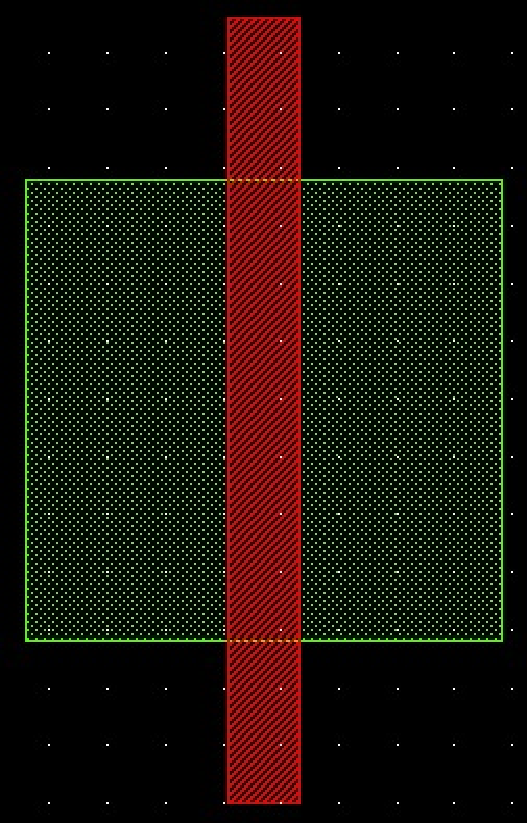
\includegraphics[width=.25\linewidth]{transistorCif}
\doxyfigcaption{A\+G\+DS example layout }
\end{DoxyImage}
\hypertarget{agds_agdsC}{}\subsection{C++}\label{agds_agdsC}
Here is the C++ code ({\ttfamily drive\+Agds.\+cpp}) used to generate the transistor.\+agds file. (Source is available in examples directory). 
\begin{DoxyCodeInclude}
\textcolor{preprocessor}{#include <string>}
\textcolor{keyword}{using namespace }\mbox{\hyperlink{namespacestd}{std}};

\textcolor{preprocessor}{#include "vlsisapd/agds/Library.h"}
\textcolor{preprocessor}{#include "vlsisapd/agds/Structure.h"}
\textcolor{preprocessor}{#include "vlsisapd/agds/Rectangle.h"}

\textcolor{keywordtype}{int} main(\textcolor{keywordtype}{int} argc, \textcolor{keywordtype}{char} * argv[]) \{
    \mbox{\hyperlink{class_a_g_d_s_1_1_library}{AGDS::Library}}* lib = \textcolor{keyword}{new} \mbox{\hyperlink{class_a_g_d_s_1_1_library}{AGDS::Library}}(\textcolor{keywordtype}{string}(\textcolor{stringliteral}{"myTestLib"}));

    lib->\mbox{\hyperlink{class_a_g_d_s_1_1_library_a0d0e972bb142f892c462bb8d7f04a50b}{setUserUnits}}(0.001);
    lib->\mbox{\hyperlink{class_a_g_d_s_1_1_library_a938acb6eb8d14aade9dba7331c75ff0a}{setPhysUnits}}(1.0E-9);

    \mbox{\hyperlink{class_a_g_d_s_1_1_rectangle}{AGDS::Rectangle}}* poly   = \textcolor{keyword}{new} \mbox{\hyperlink{class_a_g_d_s_1_1_rectangle}{AGDS::Rectangle}}( 17, 305, 150, 365, 830 );
    \mbox{\hyperlink{class_a_g_d_s_1_1_rectangle}{AGDS::Rectangle}}* active = \textcolor{keyword}{new} \mbox{\hyperlink{class_a_g_d_s_1_1_rectangle}{AGDS::Rectangle}}(  6, 130, 290, 540, 690 );

    \mbox{\hyperlink{class_a_g_d_s_1_1_structure}{AGDS::Structure}}* str = \textcolor{keyword}{new} \mbox{\hyperlink{class_a_g_d_s_1_1_structure}{AGDS::Structure}}(\textcolor{stringliteral}{"Transistor"});

    str->\mbox{\hyperlink{class_a_g_d_s_1_1_structure_a2dd203e6770f7d15d6f706867c919a60}{addElement}}(poly);
    str->\mbox{\hyperlink{class_a_g_d_s_1_1_structure_a2dd203e6770f7d15d6f706867c919a60}{addElement}}(active);

    lib->\mbox{\hyperlink{class_a_g_d_s_1_1_library_a93d333a20154e0b688ff3ff213039171}{addStructure}}(str);

    lib->\mbox{\hyperlink{class_a_g_d_s_1_1_library_a33b9d989b84857f46034085664ff3fa2}{writeToFile}}(\textcolor{stringliteral}{"./transistor.agds"});
    
    \textcolor{keywordflow}{return} 0;
\}

\end{DoxyCodeInclude}


\begin{DoxyNote}{Note}
In order to compile this code, a C\+Make\+Lists.\+txt file is provided. User must set the \$\+V\+L\+S\+I\+S\+A\+P\+D\+\_\+\+T\+OP variable before running these commands in the directory containing the C\+Make\+Lists.\+txt file\+: 
\begin{DoxyCode}
%> mkdir build; cd build
%> cmake ..
%> make
\end{DoxyCode}

\end{DoxyNote}
\hypertarget{agds_agdsPython}{}\subsection{Python}\label{agds_agdsPython}
Here is the Python code ({\ttfamily drive\+Agds.\+py}) used to generate the transistor.\+agds file. (Source is available in examples directory). 
\begin{DoxyCodeInclude}
\textcolor{keyword}{import} AGDS
lib = \mbox{\hyperlink{class_a_g_d_s_1_1_library}{AGDS.Library}}(\textcolor{stringliteral}{"myTestLib"})
lib.setUserUnits(0.001)
lib.setPhysUnits(1.0e-9)

active = \mbox{\hyperlink{class_a_g_d_s_1_1_rectangle}{AGDS.Rectangle}}( 6, 120, 290, 540, 690) \textcolor{comment}{# layer  6 corresponds to active}
poly   = \mbox{\hyperlink{class_a_g_d_s_1_1_rectangle}{AGDS.Rectangle}}(17, 305, 150, 365, 830) \textcolor{comment}{# layer 17 corresponds to polysilicium}

str = \mbox{\hyperlink{class_a_g_d_s_1_1_structure}{AGDS.Structure}}(\textcolor{stringliteral}{"Transistor"})
str.addElement(active)
str.addElement(poly)

lib.addStructure(str)
lib.writeToFile(\textcolor{stringliteral}{"./transistor.agds"})
\end{DoxyCodeInclude}


\begin{DoxyNote}{Note}
In order to run the {\ttfamily drive\+Agds.\+py} script, user must ensure that \$\+P\+Y\+T\+H\+O\+N\+P\+A\+TH variable points to the directory containing A\+G\+D\+S.\+so module. 
\end{DoxyNote}

\chapter{C\+IF Format}
\label{cif}
\Hypertarget{cif}
\hypertarget{cif_cifPres}{}\section{Presentation}\label{cif_cifPres}
The {\bfseries Caltech Intermediate Format (C\+IF)} consists in a limited set of graphic primitives used to describe the shapes on each layer of an integrated circuit (see \href{http://en.wikipedia.org/wiki/Caltech_Intermediate_Form}{\tt http\+://en.\+wikipedia.\+org/wiki/\+Caltech\+\_\+\+Intermediate\+\_\+\+Form} for more informations). ~\newline
 \hypertarget{cif_cifAutrhos}{}\subsection{Author}\label{cif_cifAutrhos}
Damien Dupuis\+: damien.\+dupuis(at)lip6(.)fr\hypertarget{cif_cifLimits}{}\subsection{Limitations}\label{cif_cifLimits}
Although the C\+IF format allows hierarchical description and supports several shapes, in this driver, we do not use hierarchy and only use Polygons.\hypertarget{cif_cifDB}{}\section{Stand alone database structure}\label{cif_cifDB}
The database consists in two simple objects \+:
\begin{DoxyItemize}
\item \mbox{\hyperlink{class_c_i_f_1_1_circuit}{C\+I\+F\+::\+Circuit}} contains all C\+IF circuit informations such as the name, the unit used, the scale and the list of all Polygons.
\item \mbox{\hyperlink{class_c_i_f_1_1_polygon}{C\+I\+F\+::\+Polygon}} describes a Polygon (a set of points).
\end{DoxyItemize}\hypertarget{cif_cifDriver}{}\subsection{Using the driver}\label{cif_cifDriver}
To drive a C\+IF file, user has to create one \mbox{\hyperlink{class_c_i_f_1_1_circuit}{C\+I\+F\+::\+Circuit}} and as many \mbox{\hyperlink{class_c_i_f_1_1_polygon}{C\+I\+F\+::\+Polygon}} as the number of shapes of the layout. The \mbox{\hyperlink{class_c_i_f_1_1_polygon}{C\+I\+F\+::\+Polygon}} objects can be created independently from for the \mbox{\hyperlink{class_c_i_f_1_1_circuit}{C\+I\+F\+::\+Circuit}} but must be finally added to the \mbox{\hyperlink{class_c_i_f_1_1_circuit}{C\+I\+F\+::\+Circuit}} using \mbox{\hyperlink{class_c_i_f_1_1_circuit_a5b37e86206e2a128ba6db4987dc09a39}{C\+I\+F\+::\+Circuit\+::add\+Polygon()}}.~\newline
Once the \mbox{\hyperlink{class_c_i_f_1_1_circuit}{C\+I\+F\+::\+Circuit}} is complete, simply call the \mbox{\hyperlink{class_c_i_f_1_1_circuit_a90c823b70c4984f302c19ceca604d101}{C\+I\+F\+::\+Circuit\+::write\+To\+File()}} method to drive the database to file.\hypertarget{cif_cifExamples}{}\section{Examples}\label{cif_cifExamples}
As said is the global presentation, V\+L\+SI S\+A\+PD project provides C++ libraries and Python modules for each supported format. In this section we present two simple code examples to drive a C\+IF file using C++ or Python. These two examples drive the same file {\ttfamily transistor.\+cif\+:} 
\begin{DoxyCodeInclude}
(CIF file written on 11-Jun-2010  13:49:44 by VLSISAPD\_CIF\_DRIVER);
(Units: micro  -  UU/DB Scale: 0.001);
DS 1 1 1;
9 Transistor;
L 6; P 130,290 540,290 540,690 130,690;
L 17; P 305,150 365,150 365,830 305,830;
DF;
C 1;
E
\end{DoxyCodeInclude}


 
\begin{DoxyImage}
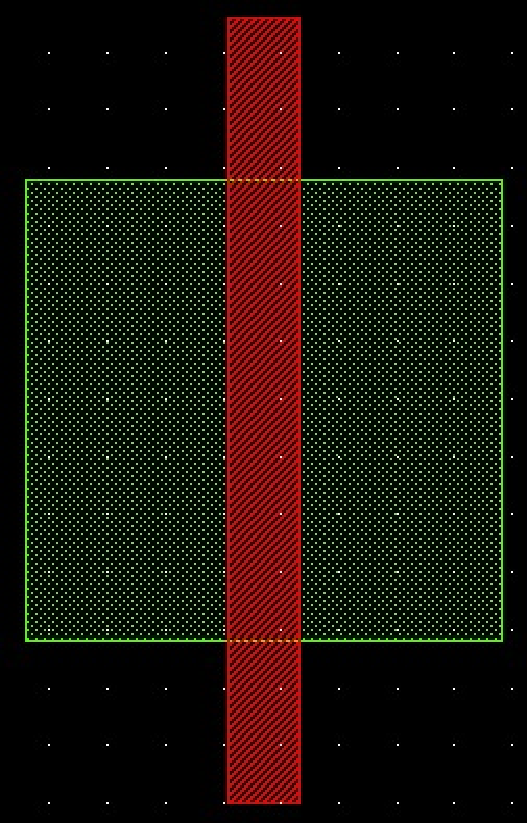
\includegraphics[width=.25\linewidth]{transistorCif}
\doxyfigcaption{C\+IF example layout }
\end{DoxyImage}
\hypertarget{cif_cifC}{}\subsection{C++}\label{cif_cifC}
Here is the C++ code ({\ttfamily drive\+Cif.\+cpp}) used to generate the transistor.\+cif file. (Source is available in examples directory). 
\begin{DoxyCodeInclude}
\textcolor{preprocessor}{#include <string>}
\textcolor{keyword}{using namespace }\mbox{\hyperlink{namespacestd}{std}};

\textcolor{preprocessor}{#include "vlsisapd/cif/Circuit.h"}
\textcolor{preprocessor}{#include "vlsisapd/cif/Polygon.h"}

\textcolor{keywordtype}{int} main(\textcolor{keywordtype}{int} argc, \textcolor{keywordtype}{char} * argv[]) \{
    \mbox{\hyperlink{class_c_i_f_1_1_circuit}{CIF::Circuit}}* circuit = \textcolor{keyword}{new} \mbox{\hyperlink{class_c_i_f_1_1_circuit}{CIF::Circuit}}(\textcolor{keywordtype}{string}(\textcolor{stringliteral}{"Transistor"}), \textcolor{keywordtype}{string}(\textcolor{stringliteral}{"micro"}),
       0.001);

    \textcolor{comment}{// Layer #6 corresponds to active}
    \mbox{\hyperlink{class_c_i_f_1_1_polygon}{CIF::Polygon}}* poly = \textcolor{keyword}{new} \mbox{\hyperlink{class_c_i_f_1_1_polygon}{CIF::Polygon}}(6);
    poly->\mbox{\hyperlink{class_c_i_f_1_1_polygon_ab3047469780327f18539907e1303ea15}{addPoint}}(130, 290);
    poly->\mbox{\hyperlink{class_c_i_f_1_1_polygon_ab3047469780327f18539907e1303ea15}{addPoint}}(540, 290);
    poly->\mbox{\hyperlink{class_c_i_f_1_1_polygon_ab3047469780327f18539907e1303ea15}{addPoint}}(540, 690);
    poly->\mbox{\hyperlink{class_c_i_f_1_1_polygon_ab3047469780327f18539907e1303ea15}{addPoint}}(130, 690);
    circuit->\mbox{\hyperlink{class_c_i_f_1_1_circuit_a5b37e86206e2a128ba6db4987dc09a39}{addPolygon}}(poly);

    \textcolor{comment}{// Layer #17 corresponds to polysilicium}
    poly = \textcolor{keyword}{new} \mbox{\hyperlink{class_c_i_f_1_1_polygon}{CIF::Polygon}}(17);
    poly->\mbox{\hyperlink{class_c_i_f_1_1_polygon_ab3047469780327f18539907e1303ea15}{addPoint}}(305, 150);
    poly->\mbox{\hyperlink{class_c_i_f_1_1_polygon_ab3047469780327f18539907e1303ea15}{addPoint}}(365, 150);
    poly->\mbox{\hyperlink{class_c_i_f_1_1_polygon_ab3047469780327f18539907e1303ea15}{addPoint}}(365, 830);
    poly->\mbox{\hyperlink{class_c_i_f_1_1_polygon_ab3047469780327f18539907e1303ea15}{addPoint}}(305, 830);
    circuit->\mbox{\hyperlink{class_c_i_f_1_1_circuit_a5b37e86206e2a128ba6db4987dc09a39}{addPolygon}}(poly);

    circuit->\mbox{\hyperlink{class_c_i_f_1_1_circuit_a90c823b70c4984f302c19ceca604d101}{writeToFile}}(\textcolor{stringliteral}{"./transistor.cif"});
    
    \textcolor{keywordflow}{return} 0;
\}

\end{DoxyCodeInclude}


\begin{DoxyNote}{Note}
In order to compile this code, a C\+Make\+Lists.\+txt file is provided. User must set the \$\+V\+L\+S\+I\+S\+A\+P\+D\+\_\+\+T\+OP variable before running these commands in the directory containing the C\+Make\+Lists.\+txt file\+: 
\begin{DoxyCode}
%> mkdir build; cd build
%> cmake ..
%> make
\end{DoxyCode}

\end{DoxyNote}
\hypertarget{cif_cifPython}{}\subsection{Python}\label{cif_cifPython}
Here is the Python code ({\ttfamily drive\+Cif.\+py}) used to generate the transistor.\+cif file. (Source is available in examples directory). 
\begin{DoxyCodeInclude}
\textcolor{keyword}{import} CIF
circuit = \mbox{\hyperlink{class_c_i_f_1_1_circuit}{CIF.Circuit}}(\textcolor{stringliteral}{"Transistor"}, \textcolor{stringliteral}{"micro"}, 0.001)
poly1 = \mbox{\hyperlink{class_c_i_f_1_1_polygon}{CIF.Polygon}}(6)
poly1.addPoint(130, 290)
poly1.addPoint(540, 290)
poly1.addPoint(540, 690)
poly1.addPoint(130, 690)
circuit.addPolygon(poly1)
    
poly2 = \mbox{\hyperlink{class_c_i_f_1_1_polygon}{CIF.Polygon}}(17)
poly2.addPoint(305, 150);
poly2.addPoint(365, 150);
poly2.addPoint(365, 830);
poly2.addPoint(305, 830);
circuit.addPolygon(poly2)

circuit.writeToFile(\textcolor{stringliteral}{"./transistor.cif"})
\end{DoxyCodeInclude}


\begin{DoxyNote}{Note}
In order to run the {\ttfamily drive\+Cif.\+py} script, user must ensure that \$\+P\+Y\+T\+H\+O\+N\+P\+A\+TH variable points to the directory containing C\+I\+F.\+so module. 
\end{DoxyNote}

\chapter{Links \& Contacts}
\label{contact}
\Hypertarget{contact}
V\+L\+SI S\+A\+PD project is developped at the {\itshape Pierre \& Marie Curie University} in {\itshape Paris}, {\itshape France} (\href{http://www.upmc.fr}{\tt http\+://www.\+upmc.\+fr}) at the L\+I\+P6 laboratory (\href{http://www.lip6.fr}{\tt http\+://www.\+lip6.\+fr}).~\newline
~\newline
 It is used by\+:
\begin{DoxyItemize}
\item Coriolis 2 Project\+: \href{http://www-soc.lip6.fr/recherche/cian/coriolis-2/}{\tt http\+://www-\/soc.\+lip6.\+fr/recherche/cian/coriolis-\/2/}
\item Chams Project\+: \href{http://www-soc.lip6.fr/recherche/cian/chams/}{\tt http\+://www-\/soc.\+lip6.\+fr/recherche/cian/chams/}~\newline
~\newline
 For any information you can contact the author of a parser / driver (if available on corresponding page) or Damien Dupuis\+: damien.\+dupuis(at)lip6(.)fr founder of the project. 
\end{DoxyItemize}
\chapter{D\+TR Format}
\label{dtr}
\Hypertarget{dtr}
\hypertarget{dtr_dtrPres}{}\section{Presentation}\label{dtr_dtrPres}
The {\bfseries Design Technology Rules (D\+TR)} format was developped as a part of the Chams Project (\href{http://www-soc.lip6.fr/recherche/cian/chams/}{\tt http\+://www-\/soc.\+lip6.\+fr/recherche/cian/chams/}). It aims at offering a generic description of layout design rules for C\+M\+OS technologies.~\newline
 \hypertarget{dtr_dtrAutrhos}{}\subsection{Author}\label{dtr_dtrAutrhos}
Damien Dupuis\+: damien.\+dupuis(at)lip6(.)fr\hypertarget{dtr_dtrLimits}{}\subsection{Limitations}\label{dtr_dtrLimits}
Only simple rules are supported at the moment. For example the minimum width of a metal layer has only one value, although it should depends on the length of the wire drawned.\hypertarget{dtr_dtrDB}{}\section{Stand alone database structure}\label{dtr_dtrDB}
The database contains four object \+:
\begin{DoxyItemize}
\item \mbox{\hyperlink{class_d_t_r_1_1_techno}{D\+T\+R\+::\+Techno}} contains generic informations such as the name of the technology and the unit used, and the list of all technologic rules.
\item \mbox{\hyperlink{class_d_t_r_1_1_rule}{D\+T\+R\+::\+Rule}} \& \mbox{\hyperlink{class_d_t_r_1_1_a_rule}{D\+T\+R\+::\+A\+Rule}} respectively describe a symmetrical and an asymmetrical rule.
\end{DoxyItemize}

The library also use the \mbox{\hyperlink{class_d_t_r_1_1_d_t_r_exception}{D\+T\+R\+::\+D\+T\+R\+Exception}} class to throw excptions.\hypertarget{dtr_dtrParser}{}\subsection{Using the parser}\label{dtr_dtrParser}
Simply load a technology with static function \mbox{\hyperlink{class_d_t_r_1_1_techno_acf863c2bdb7f1aacc4422c8155c60d17}{D\+T\+R\+::\+Techno\+::read\+From\+File()}} and then get rules (\mbox{\hyperlink{class_d_t_r_1_1_techno_a4d56a05b47bd6c51e4e18120f49b584b}{D\+T\+R\+::\+Techno\+::get\+Rule()}}) or directly values (\mbox{\hyperlink{class_d_t_r_1_1_techno_ac08e2e60dd16750551221ca908001057}{D\+T\+R\+::\+Techno\+::get\+Value()}}).\hypertarget{dtr_dtrDriver}{}\subsection{Using the driver}\label{dtr_dtrDriver}
Using the driver is very simple, user has to create a \mbox{\hyperlink{class_d_t_r_1_1_techno}{D\+T\+R\+::\+Techno}} object and simply add \mbox{\hyperlink{class_d_t_r_1_1_rule}{D\+T\+R\+::\+Rule}} or \mbox{\hyperlink{class_d_t_r_1_1_a_rule}{D\+T\+R\+::\+A\+Rule}} to it. The adding methods return the newly created Rule so user can set the rule type (\mbox{\hyperlink{class_d_t_r_1_1_rule_a3568407d7a7890c39b8c9acc1e608535}{D\+T\+R\+::\+Rule\+::set\+Type()}}) if necessary. Finally use the \mbox{\hyperlink{class_d_t_r_1_1_techno_a26b05539dd3345963b8708788b82e2cb}{D\+T\+R\+::\+Techno\+::write\+To\+File()}} method to dump the database to file.\hypertarget{dtr_dtrExamples}{}\section{Examples}\label{dtr_dtrExamples}
As said is the global presentation, V\+L\+SI S\+A\+PD project provides C++ libraries and Python modules for each supported format. In this section we present simple code examples to parse and drive a D\+TR file using C++ or Python. The D\+TR file considered is the same for all examples\+: {\ttfamily example.\+dtr.\+xml} 
\begin{DoxyCodeInclude}
<\textcolor{keywordtype}{technology} \textcolor{keyword}{name}=\textcolor{stringliteral}{"example"} \textcolor{keyword}{unit}=\textcolor{stringliteral}{"micro"} \textcolor{keyword}{version}=\textcolor{stringliteral}{"rev.A"}>
   <\textcolor{keywordtype}{physical\_rules}>
     \textcolor{comment}{<!-- transistor -->}
     <\textcolor{keywordtype}{rule}  \textcolor{keyword}{name}=\textcolor{stringliteral}{"transistorMinL"}                                         \textcolor{keyword}{value}=\textcolor{stringliteral}{"0.10"}   \textcolor{keyword}{ref}=\textcolor{stringliteral}{"ref1"}/> 
     <\textcolor{keywordtype}{rule}  \textcolor{keyword}{name}=\textcolor{stringliteral}{"transistorMinW"}                                         \textcolor{keyword}{value}=\textcolor{stringliteral}{"0.20"}   \textcolor{keyword}{ref}=\textcolor{stringliteral}{"ref2"}/>

     \textcolor{comment}{<!-- minWidth -->}
     <\textcolor{keywordtype}{rule}  \textcolor{keyword}{name}=\textcolor{stringliteral}{"minWidth"}           \textcolor{keyword}{layer}=\textcolor{stringliteral}{"metal1"}                      \textcolor{keyword}{value}=\textcolor{stringliteral}{"0.15"}   \textcolor{keyword}{ref}=\textcolor{stringliteral}{"ref3"}/>

     \textcolor{comment}{<!-- minSpacing -->}
     <\textcolor{keywordtype}{rule}  \textcolor{keyword}{name}=\textcolor{stringliteral}{"minSpacing"}         \textcolor{keyword}{layer}=\textcolor{stringliteral}{"metal1"}                      \textcolor{keyword}{value}=\textcolor{stringliteral}{"0.20"}   \textcolor{keyword}{ref}=\textcolor{stringliteral}{"ref4"}/>
     <\textcolor{keywordtype}{rule}  \textcolor{keyword}{name}=\textcolor{stringliteral}{"minSpacing"}         \textcolor{keyword}{layer1}=\textcolor{stringliteral}{"active"}   \textcolor{keyword}{layer2}=\textcolor{stringliteral}{"poly"}     \textcolor{keyword}{value}=\textcolor{stringliteral}{"0.10"}   \textcolor{keyword}{ref}=\textcolor{stringliteral}{"ref5"}/>

     \textcolor{comment}{<!-- minExtension -->}
     <\textcolor{keywordtype}{arule} \textcolor{keyword}{name}=\textcolor{stringliteral}{"minExtension"}       \textcolor{keyword}{layer1}=\textcolor{stringliteral}{"poly"}     \textcolor{keyword}{layer2}=\textcolor{stringliteral}{"active"}   \textcolor{keyword}{value}=\textcolor{stringliteral}{"0.20"}   \textcolor{keyword}{ref}=\textcolor{stringliteral}{"ref6"}/>

     \textcolor{comment}{<!-- minArea -->}
     <\textcolor{keywordtype}{rule}  \textcolor{keyword}{name}=\textcolor{stringliteral}{"minArea"}            \textcolor{keyword}{type}=\textcolor{stringliteral}{"area"}       \textcolor{keyword}{layer}=\textcolor{stringliteral}{"metal1"}    \textcolor{keyword}{value}=\textcolor{stringliteral}{"0.100"}  \textcolor{keyword}{ref}=\textcolor{stringliteral}{"ref7"}/>
  </\textcolor{keywordtype}{physical\_rules}>
</\textcolor{keywordtype}{technology}>

\end{DoxyCodeInclude}


All source codes are available in the {\ttfamily examples} directory.\hypertarget{dtr_dtrC}{}\subsection{C++}\label{dtr_dtrC}
\hypertarget{dtr_dtrParseC}{}\subsubsection{Parser}\label{dtr_dtrParseC}
The following code ({\ttfamily parse\+Dtr.\+cpp}) is an example of how to parse a D\+TR file using C++ library. 
\begin{DoxyCodeInclude}
\textcolor{preprocessor}{#include <iostream>}
\textcolor{preprocessor}{#include <string>}
\textcolor{keyword}{using namespace }\mbox{\hyperlink{namespacestd}{std}};

\textcolor{preprocessor}{#include "vlsisapd/dtr/Techno.h"}

\textcolor{keywordtype}{int} main(\textcolor{keywordtype}{int} argc, \textcolor{keywordtype}{char} * argv[]) \{
    \mbox{\hyperlink{class_d_t_r_1_1_techno}{DTR::Techno}}* techno = \mbox{\hyperlink{class_d_t_r_1_1_techno_acf863c2bdb7f1aacc4422c8155c60d17}{DTR::Techno::readFromFile}}(\textcolor{stringliteral}{"./example.dtr.xml"}
      );

    cerr << \textcolor{stringliteral}{"+-----------------------------+"} << endl
         << \textcolor{stringliteral}{"| technology:      "} << techno->\mbox{\hyperlink{class_d_t_r_1_1_techno_a3fd7335faa33dce2f87c7e50eef3e294}{getName}}()    <<   \textcolor{stringliteral}{"    |"}   << endl
         << \textcolor{stringliteral}{"| units:           "} << techno->\mbox{\hyperlink{class_d_t_r_1_1_techno_a42e12e8f890c03ebf12e754d7e489dcb}{getUnit}}()    << \textcolor{stringliteral}{"      |"} << endl
         << \textcolor{stringliteral}{"| version:         "} << techno->getVersion() << \textcolor{stringliteral}{"      |"} << endl
         << \textcolor{stringliteral}{"+-----------------------------+"} << endl << endl;

    cerr << \textcolor{stringliteral}{"transistorMinL                = "} << techno->\mbox{\hyperlink{class_d_t_r_1_1_techno_ac08e2e60dd16750551221ca908001057}{getValue}}(\textcolor{stringliteral}{"transistorMinL"}) << endl
         << \textcolor{stringliteral}{"transistorMinW                = "} << techno->\mbox{\hyperlink{class_d_t_r_1_1_techno_ad5ef5b8e444ab7a86a2e3bff7762c956}{getValueAsString}}(\textcolor{stringliteral}{"transistorMinW"}
      ) << endl
         << \textcolor{stringliteral}{"minWidth of metal1            = "} << techno->\mbox{\hyperlink{class_d_t_r_1_1_techno_ac08e2e60dd16750551221ca908001057}{getValue}}(\textcolor{stringliteral}{"minWidth"}, \textcolor{stringliteral}{"metal1"}) << endl
         << \textcolor{stringliteral}{"minSpacing of metal1          = "} << techno->\mbox{\hyperlink{class_d_t_r_1_1_techno_ac08e2e60dd16750551221ca908001057}{getValue}}(\textcolor{stringliteral}{"minWidth"}, \textcolor{stringliteral}{"metal1"}) << endl
         << \textcolor{stringliteral}{"minSpacing of active vs poly  = "} << techno->\mbox{\hyperlink{class_d_t_r_1_1_techno_ac08e2e60dd16750551221ca908001057}{getValue}}(\textcolor{stringliteral}{"minSpacing"}, \textcolor{stringliteral}{"active"}, \textcolor{stringliteral}{"poly"}) 
      << endl
         << \textcolor{stringliteral}{"minExtension active over poly = "} << techno->\mbox{\hyperlink{class_d_t_r_1_1_techno_ac08e2e60dd16750551221ca908001057}{getValue}}(\textcolor{stringliteral}{"minExtension"}, \textcolor{stringliteral}{"poly"}, \textcolor{stringliteral}{"active"}
      ) << endl
         << \textcolor{stringliteral}{"minArea of metal1             = "} << techno->\mbox{\hyperlink{class_d_t_r_1_1_techno_ac08e2e60dd16750551221ca908001057}{getValue}}(\textcolor{stringliteral}{"minArea"}, \textcolor{stringliteral}{"metal1"}) << endl;

    \textcolor{keywordflow}{return} 0;
\}

\end{DoxyCodeInclude}
\hypertarget{dtr_dtrDriveC}{}\subsubsection{Driver}\label{dtr_dtrDriveC}
This C++ code ({\ttfamily drive\+Dtr.\+cpp}) generates a out.\+dtr.\+xml file equivalent to the previous example.\+dtr.\+xml. 
\begin{DoxyCodeInclude}
\textcolor{preprocessor}{#include <string>}
\textcolor{keyword}{using namespace }\mbox{\hyperlink{namespacestd}{std}};

\textcolor{preprocessor}{#include "vlsisapd/dtr/Techno.h"}
\textcolor{preprocessor}{#include "vlsisapd/dtr/Rules.h"}

\textcolor{keywordtype}{int} main(\textcolor{keywordtype}{int} argc, \textcolor{keywordtype}{char} * argv[]) \{
    \mbox{\hyperlink{class_d_t_r_1_1_techno}{DTR::Techno}}* techno = \textcolor{keyword}{new} \mbox{\hyperlink{class_d_t_r_1_1_techno}{DTR::Techno}}(\textcolor{stringliteral}{"MyTech"}, \textcolor{stringliteral}{"micro"}, \textcolor{stringliteral}{"rev.A"});

    techno->\mbox{\hyperlink{class_d_t_r_1_1_techno_afa2c8412c365c950649b9f81661ecafd}{addRule}} (\textcolor{stringliteral}{"transistorMinL"}, 0.1 , \textcolor{stringliteral}{"ref1"});
    techno->\mbox{\hyperlink{class_d_t_r_1_1_techno_afa2c8412c365c950649b9f81661ecafd}{addRule}} (\textcolor{stringliteral}{"transistorMinW"}, 0.2 , \textcolor{stringliteral}{"ref2"});
    techno->\mbox{\hyperlink{class_d_t_r_1_1_techno_afa2c8412c365c950649b9f81661ecafd}{addRule}} (\textcolor{stringliteral}{"minWidth"}      , 0.15, \textcolor{stringliteral}{"ref3"}, \textcolor{stringliteral}{"metal1"});
    techno->\mbox{\hyperlink{class_d_t_r_1_1_techno_afa2c8412c365c950649b9f81661ecafd}{addRule}} (\textcolor{stringliteral}{"minSpacing"}    , 0.2 , \textcolor{stringliteral}{"ref4"}, \textcolor{stringliteral}{"metal1"});
    techno->\mbox{\hyperlink{class_d_t_r_1_1_techno_afa2c8412c365c950649b9f81661ecafd}{addRule}} (\textcolor{stringliteral}{"minSpacing"}    , 0.1 , \textcolor{stringliteral}{"ref5"}, \textcolor{stringliteral}{"active"}, \textcolor{stringliteral}{"poly"});
    techno->\mbox{\hyperlink{class_d_t_r_1_1_techno_a5f5a790974fe7d3b1c6f1b698ef0a818}{addARule}}(\textcolor{stringliteral}{"minExtension"}  , 0.2 , \textcolor{stringliteral}{"ref6"}, \textcolor{stringliteral}{"poly"}  , \textcolor{stringliteral}{"active"});
    
    \mbox{\hyperlink{class_d_t_r_1_1_rule}{DTR::Rule}}* rule = techno->\mbox{\hyperlink{class_d_t_r_1_1_techno_afa2c8412c365c950649b9f81661ecafd}{addRule}}(\textcolor{stringliteral}{"minArea"}, 0.1, \textcolor{stringliteral}{"ref7"}, \textcolor{stringliteral}{"metal1"});
    rule->\mbox{\hyperlink{class_d_t_r_1_1_rule_a3568407d7a7890c39b8c9acc1e608535}{setType}}(\textcolor{stringliteral}{"area"});

    techno->\mbox{\hyperlink{class_d_t_r_1_1_techno_a26b05539dd3345963b8708788b82e2cb}{writeToFile}}(\textcolor{stringliteral}{"./out.dtr.xml"});
    
    \textcolor{keywordflow}{return} 0;
\}

\end{DoxyCodeInclude}


\begin{DoxyNote}{Note}
In order to compile these codes, a C\+Make\+Lists.\+txt file is provided. User must set the \$\+V\+L\+S\+I\+S\+A\+P\+D\+\_\+\+T\+OP variable before running these commands in the directory containing the C\+Make\+Lists.\+txt file\+: 
\begin{DoxyCode}
%> mkdir build; cd build
%> cmake ..
%> make
\end{DoxyCode}

\end{DoxyNote}
\hypertarget{dtr_dtrPython}{}\subsection{Python}\label{dtr_dtrPython}
\hypertarget{dtr_dtrParsePython}{}\subsubsection{Parser}\label{dtr_dtrParsePython}
The following python script ({\ttfamily parse\+Dtr.\+py}) is an example of how to parse a D\+TR file using python module. 
\begin{DoxyCodeInclude}
\textcolor{keyword}{from} DTR \textcolor{keyword}{import} *
\textcolor{keyword}{from} decimal \textcolor{keyword}{import} Decimal

techno = Techno.readFromFile(\textcolor{stringliteral}{"./example.dtr.xml"})

\textcolor{keywordflow}{print} \textcolor{stringliteral}{"+-----------------------------+"}
\textcolor{keywordflow}{print} \textcolor{stringliteral}{"| technology:      "}+techno.get)   +  \textcolor{stringliteral}{"    |"}
\textcolor{keywordflow}{print} \textcolor{stringliteral}{"| units:           "}+techno.getUnit()   +\textcolor{stringliteral}{"      |"}
\textcolor{keywordflow}{print} \textcolor{stringliteral}{"| version:         "}+techno.getVersion()+\textcolor{stringliteral}{"      |"}
\textcolor{keywordflow}{print} \textcolor{stringliteral}{"+-----------------------------+\(\backslash\)n\(\backslash\)n"}

\textcolor{keywordflow}{print} \textcolor{stringliteral}{"transistorMinL                = %s"}%techno.getValue(\textcolor{stringliteral}{"transistorMinL"})
\textcolor{keywordflow}{print} \textcolor{stringliteral}{"transistorMinW                = %s"}%Decimal(techno.getValueAsString(\textcolor{stringliteral}{"transistorMinW"}))
\textcolor{keywordflow}{print} \textcolor{stringliteral}{"minWidth of metal1            = %s"}%techno.getValue(\textcolor{stringliteral}{"minWidth"}, \textcolor{stringliteral}{"metal1"})
\textcolor{keywordflow}{print} \textcolor{stringliteral}{"minSpacing of metal1          = %s"}%techno.getValue(\textcolor{stringliteral}{"minWidth"}, \textcolor{stringliteral}{"metal1"})
\textcolor{keywordflow}{print} \textcolor{stringliteral}{"minSpacing of active vs poly  = %s"}%techno.getValue(\textcolor{stringliteral}{"minSpacing"}, \textcolor{stringliteral}{"active"}, \textcolor{stringliteral}{"poly"})
\textcolor{keywordflow}{print} \textcolor{stringliteral}{"minExtension active over poly = %s"}%techno.getValue(\textcolor{stringliteral}{"minExtension"}, \textcolor{stringliteral}{"poly"}, \textcolor{stringliteral}{"active"})
\textcolor{keywordflow}{print} \textcolor{stringliteral}{"minArea of metal1             = %s"}%techno.getValue(\textcolor{stringliteral}{"minArea"}, \textcolor{stringliteral}{"metal1"})

\textcolor{comment}{# an example of why it is important to use Decimal in python:}
\textcolor{keywordflow}{print} techno.getValue(\textcolor{stringliteral}{"minArea"}, \textcolor{stringliteral}{"metal1"})*3-0.3 \textcolor{comment}{# returns 5.55111512313e-17}
\textcolor{keywordflow}{print} Decimal(techno.getValueAsString(\textcolor{stringliteral}{"minArea"}, \textcolor{stringliteral}{"metal1"}))*3-Decimal(\textcolor{stringliteral}{'0.3'}) \textcolor{comment}{# returns 0.000}
\end{DoxyCodeInclude}
\hypertarget{dtr_dtrDrivePython}{}\subsubsection{Driver}\label{dtr_dtrDrivePython}
This python script ({\ttfamily drive\+Dtr.\+py}) generates a out.\+dtr.\+xml file equivalent to the previous example.\+dtr.\+xml. 
\begin{DoxyCodeInclude}
\textcolor{keyword}{from} DTR \textcolor{keyword}{import} *

techno = Techno(\textcolor{stringliteral}{"myTech"}, \textcolor{stringliteral}{"micro"}, \textcolor{stringliteral}{"rev.A"})

techno.addRule (\textcolor{stringliteral}{"transistorMinL"}, 0.1 , \textcolor{stringliteral}{"ref1"})
techno.addRule (\textcolor{stringliteral}{"transistorMinW"}, 0.2 , \textcolor{stringliteral}{"ref2"})
techno.addRule (\textcolor{stringliteral}{"minWidth"}      , 0.15, \textcolor{stringliteral}{"ref3"}, \textcolor{stringliteral}{"metal1"})
techno.addRule (\textcolor{stringliteral}{"minSpacing"}    , 0.2 , \textcolor{stringliteral}{"ref4"}, \textcolor{stringliteral}{"metal1"})
techno.addRule (\textcolor{stringliteral}{"minSpacing"}    , 0.1 , \textcolor{stringliteral}{"ref5"}, \textcolor{stringliteral}{"active"}, \textcolor{stringliteral}{"poly"})
techno.addARule(\textcolor{stringliteral}{"minExtension"}  , 0.2 , \textcolor{stringliteral}{"ref6"}, \textcolor{stringliteral}{"poly"}, \textcolor{stringliteral}{"active"})

rule = techno.addRule(\textcolor{stringliteral}{"minArea"}, 0.1, \textcolor{stringliteral}{"ref7"}, \textcolor{stringliteral}{"metal1"})
rule.setType(\textcolor{stringliteral}{"area"})

techno.writeToFile(\textcolor{stringliteral}{"./out.dtr.xml"})
\end{DoxyCodeInclude}


\begin{DoxyNote}{Note}
In order to run these two scripts ({\ttfamily parse\+Dtr.\+py} \& drive\+Dtr.\+py), user must ensure that \$\+P\+Y\+T\+H\+O\+N\+P\+A\+TH variable points to the directory containing D\+T\+R.\+so module. 
\end{DoxyNote}

\chapter{O\+P\+E\+N\+C\+H\+A\+MS Format}
\label{openchams}
\Hypertarget{openchams}
\hypertarget{openchams_openChamsPres}{}\section{Presentation}\label{openchams_openChamsPres}
The {\bfseries Open\+C\+H\+A\+MS} format was developped as a part of the Chams Project (\href{http://www-soc.lip6.fr/recherche/cian/chams/}{\tt http\+://www-\/soc.\+lip6.\+fr/recherche/cian/chams/}). It aims at offering a convenient way to describe analogic circuits\textquotesingle{} netlists and is based on X\+ML. Some C\+H\+A\+MS specific informations, such as schematic properties, layout properties or sizing procedure, can be described in this format.~\newline
 \hypertarget{openchams_openChamsAutrhos}{}\subsection{Author}\label{openchams_openChamsAutrhos}
Damien Dupuis\+: damien.\+dupuis(at)lip6(.)fr\hypertarget{openchams_openChamsDB}{}\section{Stand alone database structure}\label{openchams_openChamsDB}
The database has many objects that can be arranged in five categories\+:
\begin{DoxyItemize}
\item General
\begin{DoxyItemize}
\item Open\+Chams\+::\+Circuit
\item Open\+Chams\+::\+Name
\item Open\+Chams\+::\+Open\+Chams\+Exception
\end{DoxyItemize}
\item \mbox{\hyperlink{class_netlist}{Netlist}}
\begin{DoxyItemize}
\item Open\+Chams\+::\+Netlist
\item Open\+Chams\+::\+Instance
\item Open\+Chams\+::\+Device
\item Open\+Chams\+::\+Transistor
\item Open\+Chams\+::\+Parameters
\item Open\+Chams\+::\+Net
\end{DoxyItemize}
\item \mbox{\hyperlink{class_sizing}{Sizing}}
\begin{DoxyItemize}
\item Open\+Chams\+::\+Sizing
\item Open\+Chams\+::\+Operator
\item Open\+Chams\+::\+Simul\+Model
\end{DoxyItemize}
\item \mbox{\hyperlink{class_schematic}{Schematic}}
\begin{DoxyItemize}
\item Open\+Chams\+::\+Schematic
\item Open\+Chams\+::\+Port
\item Open\+Chams\+::\+Wire
\item Open\+Chams\+::\+Wire\+Point
\item Open\+Chams\+::\+Instance\+Point
\item Open\+Chams\+::\+Port\+Point
\item Open\+Chams\+::\+Intermediate\+Point
\end{DoxyItemize}
\item \mbox{\hyperlink{class_layout}{Layout}}
\begin{DoxyItemize}
\item Open\+Chams\+::\+Layout
\item Open\+Chams\+::\+Node
\item Open\+Chams\+::\+Bloc
\item Open\+Chams\+::\+Group
\end{DoxyItemize}
\end{DoxyItemize}\hypertarget{openchams_openChamsParser}{}\subsection{Using the parser}\label{openchams_openChamsParser}
Simply load an O\+P\+E\+N\+C\+H\+A\+MS file using the static function Open\+Chams\+::\+Circuit\+::read\+From\+File() and then get the netlist object (Open\+Chams\+::\+Circuit\+::get\+Netlist()) or the sizing procedure (Open\+Chams\+::\+Circuit\+::get\+Sizing(), might be N\+U\+LL) or any other useful information (see Open\+Chams\+::\+Circuit).\hypertarget{openchams_openChamsDriver}{}\subsection{Using the driver}\label{openchams_openChamsDriver}
Using the driver is very simple, user has to create an Open\+Chams\+::\+Circuit object and simply add Open\+Chams\+::\+Netlist (mandatory) and Open\+Chams\+::\+Sizing (optionnal) or Open\+Chams\+::\+Schematic (optionnal) or Open\+Chams\+::\+Layout (optinnal) to it. Finally use the Open\+Chams\+::\+Circuit\+::write\+To\+File() method to dump the database to file.\hypertarget{openchams_openChamsExamples}{}\section{Examples}\label{openchams_openChamsExamples}
As said is the global presentation, V\+L\+SI S\+A\+PD project provides C++ libraries and Python modules for each supported format. In this section we present simple code examples to parse and drive a O\+P\+E\+N\+C\+H\+A\+MS file using C++ or Python. The O\+P\+E\+N\+C\+H\+A\+MS files considered are the same for all examples\+: {\ttfamily inverter.\+xml} and {\ttfamily buffer.\+xml} 
\begin{DoxyCodeInclude}
\end{DoxyCodeInclude}
 
\begin{DoxyCodeInclude}
\end{DoxyCodeInclude}


All source codes are available in the {\ttfamily examples} directory.\hypertarget{openchams_openChamsC}{}\subsection{C++}\label{openchams_openChamsC}
\hypertarget{openchams_openChamsParseC}{}\subsubsection{Parser}\label{openchams_openChamsParseC}
The following code ({\ttfamily parse\+Open\+Chams.\+cpp}) is an example of how to parse a O\+P\+E\+N\+C\+H\+A\+MS file using C++ library. 
\begin{DoxyCodeInclude}
\end{DoxyCodeInclude}
\hypertarget{openchams_openChamsDriveC}{}\subsubsection{Driver}\label{openchams_openChamsDriveC}
This C++ code ({\ttfamily drive\+Open\+Chams.\+cpp}) generates an inverter.\+xml file equivalent to the included one. 
\begin{DoxyCodeInclude}
\end{DoxyCodeInclude}


\begin{DoxyNote}{Note}
In order to compile these codes, a C\+Make\+Lists.\+txt file is provided. User must set the \$\+V\+L\+S\+I\+S\+A\+P\+D\+\_\+\+T\+OP variable before running these commands in the directory containing the C\+Make\+Lists.\+txt file\+: 
\begin{DoxyCode}
%> mkdir build; cd build
%> cmake ..
%> make
\end{DoxyCode}

\end{DoxyNote}
\hypertarget{openchams_openChamsPython}{}\subsection{Python}\label{openchams_openChamsPython}
\hypertarget{openchams_openChamsParsePython}{}\subsubsection{Parser}\label{openchams_openChamsParsePython}
The following python script ({\ttfamily parse\+Open\+Chams.\+py}) is an example of how to parse a O\+P\+E\+N\+C\+H\+A\+MS file using python module. 
\begin{DoxyCodeInclude}
\end{DoxyCodeInclude}
\hypertarget{openchams_openChamsDrivePython}{}\subsubsection{Driver}\label{openchams_openChamsDrivePython}
This python script ({\ttfamily drive\+Open\+Chams.\+py}) generates an inverter.\+xml file equivalent to the included one. 
\begin{DoxyCodeInclude}
\end{DoxyCodeInclude}


\begin{DoxyNote}{Note}
In order to run these two scripts ({\ttfamily parse\+Open\+Chams.\+py} \& drive\+Open\+Chams.\+py), user must ensure that \$\+P\+Y\+T\+H\+O\+N\+P\+A\+TH variable points to the directory containing O\+P\+E\+N\+C\+H\+A\+M\+S.\+so module. 
\end{DoxyNote}

\chapter{S\+P\+I\+CE Format}
\label{spice}
\Hypertarget{spice}
\hypertarget{spice_spicePres}{}\section{Presentation}\label{spice_spicePres}
The {\bfseries Spice} format was developped at the University of California, Berkeley. This parser/driver consists in a subset of S\+P\+I\+C\+E3 netlist format. (see \href{http://en.wikipedia.org/wiki/SPICE}{\tt http\+://en.\+wikipedia.\+org/wiki/\+S\+P\+I\+CE} for more informations).~\newline
 \hypertarget{spice_spiceAutrhos}{}\subsection{Author}\label{spice_spiceAutrhos}
Damien Dupuis\+: damien.\+dupuis(at)lip6(.)fr\hypertarget{spice_spiceDB}{}\section{Stand alone database structure}\label{spice_spiceDB}
The database consists in several objects\+:
\begin{DoxyItemize}
\item \mbox{\hyperlink{class_s_p_i_c_e_1_1_circuit}{S\+P\+I\+C\+E\+::\+Circuit}}
\item \mbox{\hyperlink{class_s_p_i_c_e_1_1_spice_exception}{S\+P\+I\+C\+E\+::\+Spice\+Exception}}
\item \mbox{\hyperlink{class_s_p_i_c_e_1_1_subckt}{S\+P\+I\+C\+E\+::\+Subckt}}
\item \mbox{\hyperlink{class_s_p_i_c_e_1_1_instance}{S\+P\+I\+C\+E\+::\+Instance}}
\item \mbox{\hyperlink{class_s_p_i_c_e_1_1_mosfet}{S\+P\+I\+C\+E\+::\+Mosfet}}
\item \mbox{\hyperlink{class_s_p_i_c_e_1_1_capacitor}{S\+P\+I\+C\+E\+::\+Capacitor}}
\item \mbox{\hyperlink{class_s_p_i_c_e_1_1_resistor}{S\+P\+I\+C\+E\+::\+Resistor}}
\item \mbox{\hyperlink{class_s_p_i_c_e_1_1_source}{S\+P\+I\+C\+E\+::\+Source}}
\item \mbox{\hyperlink{class_s_p_i_c_e_1_1_voltage}{S\+P\+I\+C\+E\+::\+Voltage}}
\item \mbox{\hyperlink{class_s_p_i_c_e_1_1_current}{S\+P\+I\+C\+E\+::\+Current}}
\end{DoxyItemize}\hypertarget{spice_spiceParser}{}\subsection{Using the parser}\label{spice_spiceParser}
Simply load an Spice netlist file using the static function \mbox{\hyperlink{class_s_p_i_c_e_1_1_circuit_aa8294fe7d9ceddb5653d08ecae3eaf36}{S\+P\+I\+C\+E\+::\+Circuit\+::read\+From\+File()}}.\hypertarget{spice_spiceDriver}{}\subsection{Using the driver}\label{spice_spiceDriver}
Using the driver is very simple, user has to create a \mbox{\hyperlink{class_s_p_i_c_e_1_1_circuit}{S\+P\+I\+C\+E\+::\+Circuit}} object and simply add others Spice objects like \mbox{\hyperlink{class_s_p_i_c_e_1_1_subckt}{S\+P\+I\+C\+E\+::\+Subckt}} or \mbox{\hyperlink{class_s_p_i_c_e_1_1_instance}{S\+P\+I\+C\+E\+::\+Instance}} to it. Includes, libraries and parameters can also be added to \mbox{\hyperlink{class_s_p_i_c_e_1_1_circuit}{S\+P\+I\+C\+E\+::\+Circuit}}. Finally use the S\+P\+I\+C\+E\+::\+Circuit\+::write\+To\+File() method to dump the database to file.\hypertarget{spice_spiceExamples}{}\section{Examples}\label{spice_spiceExamples}
As said is the global presentation, V\+L\+SI S\+A\+PD project provides C++ libraries and Python modules for each supported format. In this section we present simple code examples to parse and drive a S\+P\+I\+CE file using C++ or Python. The S\+P\+I\+CE file considered describes a simple Miller O\+TA\+: {\ttfamily O\+T\+A\+\_\+miller.\+spi} 
\begin{DoxyCodeInclude}
* Single-ended two-stage amplifier

.PARAM CC\_VALUE=2.8794pF
.PARAM L\_VALUE=0.340e-6

.SUBCKT currentMirrorPMOS d1 d2 s1 s2 param: l\_val=0.0 w\_val=0.0 nf\_val=1 aeq\_val=100e-6 temp\_val=27
MP3 d1 d1 s1 s1 psvt l=l\_val wf=\{w\_val/nf\_val\}  nf=nf\_val  aeq=aeq\_val tempsimu=temp\_val
MP4 d2 d1 s2 s2 psvt l=l\_val wf=\{w\_val/nf\_val\}  nf=nf\_val  aeq=aeq\_val tempsimu=temp\_val
.ENDS currentMirrorPMOS

.SUBCKT diffPairNMOS d1 d2 g1 g2 s b param: l\_val=0.0 w\_val=0.0 nf\_val=1 aeq\_val=100e-6 temp\_val=27
MN1 d1 g1 s b nsvt l=l\_val wf=\{w\_val/nf\_val\}  nf=nf\_val  aeq=aeq\_val tempsimu=temp\_val
MN2 d2 g2 s b nsvt l=l\_val wf=\{w\_val/nf\_val\}  nf=nf\_val  aeq=aeq\_val tempsimu=temp\_val
.ENDS diffPairNMOS

XCM   1    2   vdd vdd         currentMirrorPMOS  l\_val=L\_VALUE  w\_val=3.889618e-06  nf\_val=2
XDP   1    2   vim vip 3   vss diffPairNMOS       l\_val=L\_VALUE  w\_val=7.683346e-07  nf\_val=4
MP6   vout 2   vdd vdd         psvt               l\_val=L\_VALUE  w\_val=3.558995e-05  nf\_val=20
MN5   3    4   vss vss         nsvt               l\_val=L\_VALUE  w\_val=2.536703e-06  nf\_val=4 
MN7   vout 4   vss vss         nsvt               l\_val=L\_VALUE  w\_val=1.069083e-05  nf\_val=16
MN8   4    4   vss vss         nsvt               l\_val=L\_VALUE  w\_val=2.536703e-06  nf\_val=4 

CC1   vout 2   CC\_VALUE

.END
\end{DoxyCodeInclude}


All source codes are available in the {\ttfamily examples} directory.\hypertarget{spice_spiceC}{}\subsection{C++}\label{spice_spiceC}
\hypertarget{spice_spiceParseC}{}\subsubsection{Parser}\label{spice_spiceParseC}
The following code ({\ttfamily parse\+Spice.\+cpp}) is an example of how to parse a S\+P\+I\+CE file using C++ library. 
\begin{DoxyCodeInclude}
\textcolor{preprocessor}{#include <cstdlib>}
\textcolor{preprocessor}{#include <iostream>}
\textcolor{preprocessor}{#include <string>}
\textcolor{preprocessor}{#include <map>}
\textcolor{preprocessor}{#include <vector>}
\textcolor{keyword}{using namespace }\mbox{\hyperlink{namespacestd}{std}};

\textcolor{preprocessor}{#include "vlsisapd/spice/Circuit.h"}
\textcolor{preprocessor}{#include "vlsisapd/spice/SpiceException.h"}
\textcolor{preprocessor}{#include "vlsisapd/spice/Sources.h"}
\textcolor{preprocessor}{#include "vlsisapd/spice/Subckt.h"}
\textcolor{preprocessor}{#include "vlsisapd/spice/Instances.h"}

\textcolor{keywordtype}{int} main(\textcolor{keywordtype}{int} argc, \textcolor{keywordtype}{char} * argv[]) \{
    \textcolor{keywordtype}{string} file = \textcolor{stringliteral}{""};
    \textcolor{keywordflow}{if} (argc == 1)
        file = \textcolor{stringliteral}{"./OTA.cir"};
    \textcolor{keywordflow}{else} \textcolor{keywordflow}{if} (argc == 2)
        file = argv[1];
    \textcolor{keywordflow}{else} \{
        cerr << \textcolor{stringliteral}{"Usage: parseSpice [filename]"} << endl;
        exit(1);
    \}

    \mbox{\hyperlink{class_s_p_i_c_e_1_1_circuit}{SPICE::Circuit}}* circuit = NULL;
    \textcolor{keywordflow}{try} \{
        circuit = \mbox{\hyperlink{class_s_p_i_c_e_1_1_circuit_aa8294fe7d9ceddb5653d08ecae3eaf36}{SPICE::Circuit::readFromFile}}(file);
    \} \textcolor{keywordflow}{catch} (\mbox{\hyperlink{class_s_p_i_c_e_1_1_spice_exception}{SPICE::SpiceException}}& e) \{
        cerr << e.what() << endl;
        exit(48);
    \}

\textcolor{comment}{//    if (!circuit) cerr << "circuit is NULL !!" << endl;}
    \textcolor{comment}{// TITLE}
    cerr << \textcolor{stringliteral}{"+ "} << circuit->\mbox{\hyperlink{class_s_p_i_c_e_1_1_circuit_ad19721dd878c04c854a72af12d785741}{getTitle}}() << endl;
    \textcolor{comment}{// INCLUDES}
    vector<string> includes = circuit->\mbox{\hyperlink{class_s_p_i_c_e_1_1_circuit_a312beaf640e84589e6644820355c8ed6}{getIncludes}}();
    \textcolor{keywordflow}{if} (includes.size()) \{
        cerr << \textcolor{stringliteral}{"| + includes"} << endl;
        \textcolor{keywordflow}{for} (\textcolor{keywordtype}{size\_t} i = 0 ; i < includes.size() ; i++)
            cerr << \textcolor{stringliteral}{"| | "} << includes[i] << endl;
    \}
    \textcolor{comment}{// LIBRARIES}
    vector<pair<string, string> > libs = circuit->\mbox{\hyperlink{class_s_p_i_c_e_1_1_circuit_a3e6a71a711e4796470f1a2a1dc42aef6}{getLibraries}}();
    \textcolor{keywordflow}{if} (libs.size()) \{
        cerr << \textcolor{stringliteral}{"| + libraries"} << endl;
        \textcolor{keywordflow}{for} (\textcolor{keywordtype}{size\_t} i = 0 ; i < libs.size() ; i++)
            cerr << \textcolor{stringliteral}{"| | "} << libs[i].first << \textcolor{stringliteral}{" "} << libs[i].second << endl;
    \}
    \textcolor{comment}{// PARAMETERS}
    map<string, string> params = circuit->\mbox{\hyperlink{class_s_p_i_c_e_1_1_circuit_a4c46676f9ead2db537a0dd963b4f08f1}{getParameters}}();
    \textcolor{keywordflow}{if} (params.size()) \{
        cerr << \textcolor{stringliteral}{"| + parameters"} << endl;
        \textcolor{keywordflow}{for} (map<string, string>::const\_iterator it = params.begin() ; it != params.end() ; ++it)
            cerr << \textcolor{stringliteral}{"| | "} << (*it).first << \textcolor{stringliteral}{" = "} << (*it).second << endl;
    \}
    \textcolor{comment}{// OPTIONS}
    map<string, string> opts = circuit->\mbox{\hyperlink{class_s_p_i_c_e_1_1_circuit_a4ee11ef79ef893c5621e0e7d26a7f9a7}{getOptions}}();
    \textcolor{keywordflow}{if} (opts.size()) \{
        cerr << \textcolor{stringliteral}{"| + options"} << endl;
        \textcolor{keywordflow}{for} (map<string, string>::const\_iterator it = opts.begin() ; it != opts.end() ; ++it)
            cerr << \textcolor{stringliteral}{"| | "} << (*it).first << \textcolor{stringliteral}{" = "} << (*it).second << endl;
    \}
    \textcolor{comment}{// SOURCES}
    vector<SPICE::Source*> sources = circuit->\mbox{\hyperlink{class_s_p_i_c_e_1_1_circuit_ac18caa525ed386c44874ee643c88e27b}{getSources}}();
    \textcolor{keywordflow}{if} (sources.size()) \{
        cerr << \textcolor{stringliteral}{"| + sources"} << endl;
        \textcolor{keywordflow}{for} (\textcolor{keywordtype}{size\_t} i = 0 ; i < sources.size() ; i++) \{
            \mbox{\hyperlink{class_s_p_i_c_e_1_1_source}{SPICE::Source}}* s = sources[i];
            cerr << \textcolor{stringliteral}{"| | "} <<  s->\mbox{\hyperlink{class_s_p_i_c_e_1_1_source_ac0fc966d4386ddb71d99361e3fccb311}{getName}}() << \textcolor{stringliteral}{" "} << s->\mbox{\hyperlink{class_s_p_i_c_e_1_1_source_a1adb347b9a2c2da556e4417ab0eec0e1}{getPositive}}() << \textcolor{stringliteral}{" "} << s->
      \mbox{\hyperlink{class_s_p_i_c_e_1_1_source_a8b4ab73ed1d99c533aa22af0a37ebb0d}{getNegative}}() << \textcolor{stringliteral}{" "} << s->\mbox{\hyperlink{class_s_p_i_c_e_1_1_source_a4c052cb2622c580a250b2c783a436882}{getValue}}() << endl;
        \}

    \}
    \textcolor{comment}{// SUBCKTS}
    vector<SPICE::Subckt*> subs = circuit->\mbox{\hyperlink{class_s_p_i_c_e_1_1_circuit_adcc4ca0de68f8ee05f0d5db3b7604930}{getSubckts}}();
    \textcolor{keywordflow}{if} (subs.size()) \{
        cerr << \textcolor{stringliteral}{"| + subckts"} << endl;
        \textcolor{keywordflow}{for} (\textcolor{keywordtype}{size\_t} i = 0 ; i < subs.size() ; i++) \{
            \mbox{\hyperlink{class_s_p_i_c_e_1_1_subckt}{SPICE::Subckt}}* sub = subs[i];
            cerr << \textcolor{stringliteral}{"| | + "} << sub->\mbox{\hyperlink{class_s_p_i_c_e_1_1_subckt_af55b1fe10eacd22c7ff3544b5ed32ef3}{getName}}(); 
            \textcolor{keywordflow}{for} (\textcolor{keywordtype}{size\_t} j = 0 ; j < sub->\mbox{\hyperlink{class_s_p_i_c_e_1_1_subckt_a5df00fe6eb5e287abef28c76ce88bd1e}{getInterfaces}}().size() ; j++)
                cerr << \textcolor{stringliteral}{" "} << sub->\mbox{\hyperlink{class_s_p_i_c_e_1_1_subckt_a5df00fe6eb5e287abef28c76ce88bd1e}{getInterfaces}}()[j];
            \textcolor{keywordflow}{if} (sub->\mbox{\hyperlink{class_s_p_i_c_e_1_1_subckt_aee7d59083b78d31ac5c19ab508da91e0}{getParameters}}().size()) \{
                cerr << \textcolor{stringliteral}{" param:"};
                \textcolor{keywordflow}{for} (map<string, string>::const\_iterator it = sub->\mbox{\hyperlink{class_s_p_i_c_e_1_1_subckt_aee7d59083b78d31ac5c19ab508da91e0}{getParameters}}().begin() ; 
      it != sub->\mbox{\hyperlink{class_s_p_i_c_e_1_1_subckt_aee7d59083b78d31ac5c19ab508da91e0}{getParameters}}().end() ; ++it)
                    cerr << \textcolor{stringliteral}{" "} << (*it).first << \textcolor{stringliteral}{"="} << (*it).second;
            \}
            cerr << endl;
            \textcolor{keywordflow}{for} (\textcolor{keywordtype}{size\_t} j = 0 ; j < sub->\mbox{\hyperlink{class_s_p_i_c_e_1_1_subckt_a8e6e58ffab876152a740092520c35d73}{getInstances}}().size() ; j++) \{
                \mbox{\hyperlink{class_s_p_i_c_e_1_1_instance}{SPICE::Instance}}* inst = sub->\mbox{\hyperlink{class_s_p_i_c_e_1_1_subckt_a8e6e58ffab876152a740092520c35d73}{getInstances}}()[j];
                cerr << \textcolor{stringliteral}{"| | | + "} << inst->\mbox{\hyperlink{class_s_p_i_c_e_1_1_instance_ac0fc966d4386ddb71d99361e3fccb311}{getName}}();
                \textcolor{keywordflow}{if} (dynamic\_cast<SPICE::Mosfet*>(inst)) \{
                    \mbox{\hyperlink{class_s_p_i_c_e_1_1_mosfet}{SPICE::Mosfet}}* mos = \textcolor{keyword}{static\_cast<}\mbox{\hyperlink{class_s_p_i_c_e_1_1_mosfet}{SPICE::Mosfet}}*\textcolor{keyword}{>}(inst);
                    cerr << \textcolor{stringliteral}{" "} << mos->\mbox{\hyperlink{class_s_p_i_c_e_1_1_mosfet_a7265f0565b8368070a3f09c6197a4e9b}{getDrain}}() << \textcolor{stringliteral}{" "} << mos->
      \mbox{\hyperlink{class_s_p_i_c_e_1_1_mosfet_a796d77755aac0828419f55ba2226bf15}{getGrid}}() << \textcolor{stringliteral}{" "} << mos->\mbox{\hyperlink{class_s_p_i_c_e_1_1_mosfet_a1791f52b6b5043823c6f3376e8453e3a}{getSource}}() << \textcolor{stringliteral}{" "} << mos->\mbox{\hyperlink{class_s_p_i_c_e_1_1_mosfet_a56484a169335450d6043ee20086ead93}{getBulk}}() << \textcolor{stringliteral}{" "} << mos->
      \mbox{\hyperlink{class_s_p_i_c_e_1_1_instance_afc74cbe93df9c473a53db83a325f8f9d}{getModel}}();
                    \textcolor{keywordtype}{int} k = 0;
                    \textcolor{keywordflow}{for} (map<string, string>::const\_iterator it =mos->
      \mbox{\hyperlink{class_s_p_i_c_e_1_1_instance_aee7d59083b78d31ac5c19ab508da91e0}{getParameters}}().begin() ; it != mos->\mbox{\hyperlink{class_s_p_i_c_e_1_1_instance_aee7d59083b78d31ac5c19ab508da91e0}{getParameters}}().end(); ++it, k++) \{
                        \textcolor{keywordflow}{if} (k%6 == 0)
                            cerr << endl << \textcolor{stringliteral}{"| | | | +"};
                        cerr << \textcolor{stringliteral}{" "} << (*it).first << \textcolor{stringliteral}{"="} << (*it).second;
                    \}
                \} \textcolor{keywordflow}{else} \textcolor{keywordflow}{if} (dynamic\_cast<SPICE::Resistor*>(inst)) \{
                    \mbox{\hyperlink{class_s_p_i_c_e_1_1_resistor}{SPICE::Resistor}}* res = \textcolor{keyword}{static\_cast<}
      \mbox{\hyperlink{class_s_p_i_c_e_1_1_resistor}{SPICE::Resistor}}*\textcolor{keyword}{>}(inst);
                    cerr << \textcolor{stringliteral}{" "} << res->\mbox{\hyperlink{class_s_p_i_c_e_1_1_resistor_ab57aa52f48a5a56c89dd49eae66c1a0f}{getFirst}}() << \textcolor{stringliteral}{" "} << res->
      \mbox{\hyperlink{class_s_p_i_c_e_1_1_resistor_a9665313821b2fca41e14b9865133af7f}{getSecond}}() << \textcolor{stringliteral}{" "} << res->\mbox{\hyperlink{class_s_p_i_c_e_1_1_resistor_a4c052cb2622c580a250b2c783a436882}{getValue}}();
                \} \textcolor{keywordflow}{else} \textcolor{keywordflow}{if} (dynamic\_cast<SPICE::Capacitor*>(inst)) \{
                    \mbox{\hyperlink{class_s_p_i_c_e_1_1_capacitor}{SPICE::Capacitor}}* capa = \textcolor{keyword}{static\_cast<}
      \mbox{\hyperlink{class_s_p_i_c_e_1_1_capacitor}{SPICE::Capacitor}}*\textcolor{keyword}{>}(inst);
                    cerr << \textcolor{stringliteral}{" "} << capa->\mbox{\hyperlink{class_s_p_i_c_e_1_1_capacitor_a1adb347b9a2c2da556e4417ab0eec0e1}{getPositive}}() << \textcolor{stringliteral}{" "} << capa->
      \mbox{\hyperlink{class_s_p_i_c_e_1_1_capacitor_a8b4ab73ed1d99c533aa22af0a37ebb0d}{getNegative}}() << \textcolor{stringliteral}{" "} << capa->\mbox{\hyperlink{class_s_p_i_c_e_1_1_capacitor_a4c052cb2622c580a250b2c783a436882}{getValue}}();
                \} \textcolor{keywordflow}{else} \{
                    \textcolor{keywordflow}{for} (\textcolor{keywordtype}{size\_t} k = 0 ; k < inst->\mbox{\hyperlink{class_s_p_i_c_e_1_1_instance_acce8940edeaa3d79c522006f987e0711}{getConnectors}}().size() ; k++)
                        cerr << \textcolor{stringliteral}{" "} << inst->\mbox{\hyperlink{class_s_p_i_c_e_1_1_instance_acce8940edeaa3d79c522006f987e0711}{getConnectors}}()[k];
                    cerr << \textcolor{stringliteral}{" "} << inst->\mbox{\hyperlink{class_s_p_i_c_e_1_1_instance_afc74cbe93df9c473a53db83a325f8f9d}{getModel}}();
                    \textcolor{keywordtype}{int} l = 0;
                    \textcolor{keywordflow}{for} (map<string, string>::const\_iterator it = inst->
      \mbox{\hyperlink{class_s_p_i_c_e_1_1_instance_aee7d59083b78d31ac5c19ab508da91e0}{getParameters}}().begin() ; it != inst->\mbox{\hyperlink{class_s_p_i_c_e_1_1_instance_aee7d59083b78d31ac5c19ab508da91e0}{getParameters}}().end() ; ++it, l++) \{
                        \textcolor{keywordflow}{if} (l%6 == 0)
                            cerr << endl << \textcolor{stringliteral}{"| | | | +"};
                        cerr << \textcolor{stringliteral}{" "} << (*it).first << \textcolor{stringliteral}{"="} << (*it).second;
                    \}
                \}
                cerr << endl;
            \}
        \}
    \}
    \textcolor{comment}{// INSTANCES}
    vector<SPICE::Instance*> insts = circuit->\mbox{\hyperlink{class_s_p_i_c_e_1_1_circuit_a8e6e58ffab876152a740092520c35d73}{getInstances}}();
    \textcolor{keywordflow}{if} (insts.size()) \{
        cerr << \textcolor{stringliteral}{"| + instances"} << endl;
        \textcolor{keywordflow}{for} (\textcolor{keywordtype}{size\_t} i = 0 ; i < insts.size() ; i++) \{
            \mbox{\hyperlink{class_s_p_i_c_e_1_1_instance}{SPICE::Instance}}* inst = insts[i];
            cerr << \textcolor{stringliteral}{"| | + "} << inst->\mbox{\hyperlink{class_s_p_i_c_e_1_1_instance_ac0fc966d4386ddb71d99361e3fccb311}{getName}}();
            \textcolor{keywordflow}{if} (dynamic\_cast<SPICE::Mosfet*>(inst)) \{
                \mbox{\hyperlink{class_s_p_i_c_e_1_1_mosfet}{SPICE::Mosfet}}* mos = \textcolor{keyword}{static\_cast<}\mbox{\hyperlink{class_s_p_i_c_e_1_1_mosfet}{SPICE::Mosfet}}*\textcolor{keyword}{>}(inst);
                cerr << \textcolor{stringliteral}{" "} << mos->\mbox{\hyperlink{class_s_p_i_c_e_1_1_mosfet_a7265f0565b8368070a3f09c6197a4e9b}{getDrain}}() << \textcolor{stringliteral}{" "} << mos->\mbox{\hyperlink{class_s_p_i_c_e_1_1_mosfet_a796d77755aac0828419f55ba2226bf15}{getGrid}}() << \textcolor{stringliteral}{" "} << mos->
      \mbox{\hyperlink{class_s_p_i_c_e_1_1_mosfet_a1791f52b6b5043823c6f3376e8453e3a}{getSource}}() << \textcolor{stringliteral}{" "} << mos->\mbox{\hyperlink{class_s_p_i_c_e_1_1_mosfet_a56484a169335450d6043ee20086ead93}{getBulk}}() << \textcolor{stringliteral}{" "} << mos->\mbox{\hyperlink{class_s_p_i_c_e_1_1_instance_afc74cbe93df9c473a53db83a325f8f9d}{getModel}}();
                \textcolor{keywordtype}{int} j = 0;
                \textcolor{keywordflow}{for} (map<string, string>::const\_iterator it =mos->\mbox{\hyperlink{class_s_p_i_c_e_1_1_instance_aee7d59083b78d31ac5c19ab508da91e0}{getParameters}}().begin() ; it
       != mos->\mbox{\hyperlink{class_s_p_i_c_e_1_1_instance_aee7d59083b78d31ac5c19ab508da91e0}{getParameters}}().end(); ++it, j++) \{
                    \textcolor{keywordflow}{if} (j%6 == 0)
                        cerr << endl << \textcolor{stringliteral}{"| | | | +"};
                    cerr << \textcolor{stringliteral}{" "} << (*it).first << \textcolor{stringliteral}{"="} << (*it).second;
                \}
            \} \textcolor{keywordflow}{else} \textcolor{keywordflow}{if} (dynamic\_cast<SPICE::Resistor*>(inst)) \{
                \mbox{\hyperlink{class_s_p_i_c_e_1_1_resistor}{SPICE::Resistor}}* res = \textcolor{keyword}{static\_cast<}
      \mbox{\hyperlink{class_s_p_i_c_e_1_1_resistor}{SPICE::Resistor}}*\textcolor{keyword}{>}(inst);
                cerr << \textcolor{stringliteral}{" "} << res->\mbox{\hyperlink{class_s_p_i_c_e_1_1_resistor_ab57aa52f48a5a56c89dd49eae66c1a0f}{getFirst}}() << \textcolor{stringliteral}{" "} << res->\mbox{\hyperlink{class_s_p_i_c_e_1_1_resistor_a9665313821b2fca41e14b9865133af7f}{getSecond}}() << \textcolor{stringliteral}{" "} << res->
      \mbox{\hyperlink{class_s_p_i_c_e_1_1_resistor_a4c052cb2622c580a250b2c783a436882}{getValue}}();
            \} \textcolor{keywordflow}{else} \textcolor{keywordflow}{if} (dynamic\_cast<SPICE::Capacitor*>(inst)) \{
                \mbox{\hyperlink{class_s_p_i_c_e_1_1_capacitor}{SPICE::Capacitor}}* capa = \textcolor{keyword}{static\_cast<}
      \mbox{\hyperlink{class_s_p_i_c_e_1_1_capacitor}{SPICE::Capacitor}}*\textcolor{keyword}{>}(inst);
                cerr << \textcolor{stringliteral}{" "} << capa->\mbox{\hyperlink{class_s_p_i_c_e_1_1_capacitor_a1adb347b9a2c2da556e4417ab0eec0e1}{getPositive}}() << \textcolor{stringliteral}{" "} << capa->
      \mbox{\hyperlink{class_s_p_i_c_e_1_1_capacitor_a8b4ab73ed1d99c533aa22af0a37ebb0d}{getNegative}}() << \textcolor{stringliteral}{" "} << capa->\mbox{\hyperlink{class_s_p_i_c_e_1_1_capacitor_a4c052cb2622c580a250b2c783a436882}{getValue}}();
            \} \textcolor{keywordflow}{else} \{
                \textcolor{keywordflow}{for} (\textcolor{keywordtype}{size\_t} k = 0 ; k < inst->\mbox{\hyperlink{class_s_p_i_c_e_1_1_instance_acce8940edeaa3d79c522006f987e0711}{getConnectors}}().size() ; k++)
                    cerr << \textcolor{stringliteral}{" "} << inst->\mbox{\hyperlink{class_s_p_i_c_e_1_1_instance_acce8940edeaa3d79c522006f987e0711}{getConnectors}}()[k];
                cerr << \textcolor{stringliteral}{" "} << inst->\mbox{\hyperlink{class_s_p_i_c_e_1_1_instance_afc74cbe93df9c473a53db83a325f8f9d}{getModel}}();
                \textcolor{keywordtype}{int} l = 0;
                \textcolor{keywordflow}{for} (map<string, string>::const\_iterator it = inst->
      \mbox{\hyperlink{class_s_p_i_c_e_1_1_instance_aee7d59083b78d31ac5c19ab508da91e0}{getParameters}}().begin() ; it != inst->\mbox{\hyperlink{class_s_p_i_c_e_1_1_instance_aee7d59083b78d31ac5c19ab508da91e0}{getParameters}}().end() ; ++it, l++) \{
                    \textcolor{keywordflow}{if} (l%6 == 0)
                        cerr << endl << \textcolor{stringliteral}{"| | | +"};
                    cerr << \textcolor{stringliteral}{" "} << (*it).first << \textcolor{stringliteral}{"="} << (*it).second;
                \}
            \}
            cerr << endl;
        \}
    \}
    \textcolor{keywordflow}{return} 0;
\}

\end{DoxyCodeInclude}
\hypertarget{spice_spiceDriveC}{}\subsubsection{Driver}\label{spice_spiceDriveC}
This C++ code ({\ttfamily drive\+Spice.\+cpp}) generates an my\+O\+T\+A.\+spi file equivalent to the included one. 
\begin{DoxyCodeInclude}
\textcolor{preprocessor}{#include <string>}
\textcolor{keyword}{using namespace }\mbox{\hyperlink{namespacestd}{std}};

\textcolor{preprocessor}{#include "vlsisapd/spice/Circuit.h"}
\textcolor{preprocessor}{#include "vlsisapd/spice/Subckt.h"}
\textcolor{preprocessor}{#include "vlsisapd/spice/Instances.h"}

\textcolor{keywordtype}{int} main(\textcolor{keywordtype}{int} argc, \textcolor{keywordtype}{char} * argv[]) \{
    \mbox{\hyperlink{class_s_p_i_c_e_1_1_circuit}{SPICE::Circuit}}* circuit = \textcolor{keyword}{new} \mbox{\hyperlink{class_s_p_i_c_e_1_1_circuit}{SPICE::Circuit}}();
    circuit->\mbox{\hyperlink{class_s_p_i_c_e_1_1_circuit_a798df9ebd558e22c85eeceb5202e3123}{setTitle}}(\textcolor{stringliteral}{"* Single-ended two-stage amplifier"});

    \textcolor{comment}{// PARAMS}
    circuit->\mbox{\hyperlink{class_s_p_i_c_e_1_1_circuit_ab3ab147a16bc490ce96db905a4ca271c}{addParameter}}(\textcolor{stringliteral}{"CC\_VALUE"}, \textcolor{stringliteral}{"2.8794pF"});
    circuit->\mbox{\hyperlink{class_s_p_i_c_e_1_1_circuit_ab3ab147a16bc490ce96db905a4ca271c}{addParameter}}(\textcolor{stringliteral}{"L\_VALUE"} , \textcolor{stringliteral}{"0.340e-6"});

    \textcolor{comment}{// SUBCKTS}
    \textcolor{comment}{// CurrentMirror}
    \mbox{\hyperlink{class_s_p_i_c_e_1_1_subckt}{SPICE::Subckt}}* CM = circuit->\mbox{\hyperlink{class_s_p_i_c_e_1_1_circuit_a0d1352e46d4537ce1e5f651de40e91a6}{addSubckt}}(\textcolor{stringliteral}{"currentMirrorPMOS"});
    CM->\mbox{\hyperlink{class_s_p_i_c_e_1_1_subckt_ac162264683fa3d9b3384d3e8cc291fa2}{addInterface}}(\textcolor{stringliteral}{"d1"});
    CM->\mbox{\hyperlink{class_s_p_i_c_e_1_1_subckt_ac162264683fa3d9b3384d3e8cc291fa2}{addInterface}}(\textcolor{stringliteral}{"d2"});
    CM->\mbox{\hyperlink{class_s_p_i_c_e_1_1_subckt_ac162264683fa3d9b3384d3e8cc291fa2}{addInterface}}(\textcolor{stringliteral}{"s1"});
    CM->\mbox{\hyperlink{class_s_p_i_c_e_1_1_subckt_ac162264683fa3d9b3384d3e8cc291fa2}{addInterface}}(\textcolor{stringliteral}{"s2"});
    CM->\mbox{\hyperlink{class_s_p_i_c_e_1_1_subckt_ab3ab147a16bc490ce96db905a4ca271c}{addParameter}}(\textcolor{stringliteral}{"l\_val"}   , \textcolor{stringliteral}{"0.0"}   );
    CM->\mbox{\hyperlink{class_s_p_i_c_e_1_1_subckt_ab3ab147a16bc490ce96db905a4ca271c}{addParameter}}(\textcolor{stringliteral}{"w\_val"}   , \textcolor{stringliteral}{"0.0"}   );
    CM->\mbox{\hyperlink{class_s_p_i_c_e_1_1_subckt_ab3ab147a16bc490ce96db905a4ca271c}{addParameter}}(\textcolor{stringliteral}{"nf\_val"}  , \textcolor{stringliteral}{"1"}     );
    CM->\mbox{\hyperlink{class_s_p_i_c_e_1_1_subckt_ab3ab147a16bc490ce96db905a4ca271c}{addParameter}}(\textcolor{stringliteral}{"aeq\_val"} , \textcolor{stringliteral}{"100e-6"});
    CM->\mbox{\hyperlink{class_s_p_i_c_e_1_1_subckt_ab3ab147a16bc490ce96db905a4ca271c}{addParameter}}(\textcolor{stringliteral}{"temp\_val"}, \textcolor{stringliteral}{"27"}    );

    \mbox{\hyperlink{class_s_p_i_c_e_1_1_instance}{SPICE::Instance}}* cmP3 = \textcolor{keyword}{new} \mbox{\hyperlink{class_s_p_i_c_e_1_1_mosfet}{SPICE::Mosfet}}(\textcolor{stringliteral}{"P3"}, \textcolor{stringliteral}{"d1"}, \textcolor{stringliteral}{"d1"}, \textcolor{stringliteral}{"s1"}, \textcolor{stringliteral}{"s1"}, \textcolor{stringliteral}{"
      psvt"});
    cmP3->\mbox{\hyperlink{class_s_p_i_c_e_1_1_instance_a8d69bbbea5ece0949e100c464e412f20}{addParameter}}(\textcolor{stringliteral}{"l"}       , \textcolor{stringliteral}{"l\_val"}         );
    cmP3->\mbox{\hyperlink{class_s_p_i_c_e_1_1_instance_a8d69bbbea5ece0949e100c464e412f20}{addParameter}}(\textcolor{stringliteral}{"wf"}      , \textcolor{stringliteral}{"\{w\_val/nf\_val\}"});
    cmP3->\mbox{\hyperlink{class_s_p_i_c_e_1_1_instance_a8d69bbbea5ece0949e100c464e412f20}{addParameter}}(\textcolor{stringliteral}{"nf"}      , \textcolor{stringliteral}{"nf\_val"}        );
    cmP3->\mbox{\hyperlink{class_s_p_i_c_e_1_1_instance_a8d69bbbea5ece0949e100c464e412f20}{addParameter}}(\textcolor{stringliteral}{"aeq"}     , \textcolor{stringliteral}{"aeq\_val"}       );
    cmP3->\mbox{\hyperlink{class_s_p_i_c_e_1_1_instance_a8d69bbbea5ece0949e100c464e412f20}{addParameter}}(\textcolor{stringliteral}{"tempsimu"}, \textcolor{stringliteral}{"temp\_val"}      );
    CM->\mbox{\hyperlink{class_s_p_i_c_e_1_1_subckt_a7bb4a4532643568ab1ac2c229185a88e}{addInstance}}(cmP3);

    \mbox{\hyperlink{class_s_p_i_c_e_1_1_instance}{SPICE::Instance}}* cmP4 = \textcolor{keyword}{new} \mbox{\hyperlink{class_s_p_i_c_e_1_1_mosfet}{SPICE::Mosfet}}(\textcolor{stringliteral}{"P4"}, \textcolor{stringliteral}{"d2"}, \textcolor{stringliteral}{"d1"}, \textcolor{stringliteral}{"s2"}, \textcolor{stringliteral}{"s2"}, \textcolor{stringliteral}{"
      psvt"});
    cmP4->\mbox{\hyperlink{class_s_p_i_c_e_1_1_instance_a8d69bbbea5ece0949e100c464e412f20}{addParameter}}(\textcolor{stringliteral}{"l"}       , \textcolor{stringliteral}{"l\_val"}         );
    cmP4->\mbox{\hyperlink{class_s_p_i_c_e_1_1_instance_a8d69bbbea5ece0949e100c464e412f20}{addParameter}}(\textcolor{stringliteral}{"wf"}      , \textcolor{stringliteral}{"\{w\_val/nf\_val\}"});
    cmP4->\mbox{\hyperlink{class_s_p_i_c_e_1_1_instance_a8d69bbbea5ece0949e100c464e412f20}{addParameter}}(\textcolor{stringliteral}{"nf"}      , \textcolor{stringliteral}{"nf\_val"}        );
    cmP4->\mbox{\hyperlink{class_s_p_i_c_e_1_1_instance_a8d69bbbea5ece0949e100c464e412f20}{addParameter}}(\textcolor{stringliteral}{"aeq"}     , \textcolor{stringliteral}{"aeq\_val"}       );
    cmP4->\mbox{\hyperlink{class_s_p_i_c_e_1_1_instance_a8d69bbbea5ece0949e100c464e412f20}{addParameter}}(\textcolor{stringliteral}{"tempsimu"}, \textcolor{stringliteral}{"temp\_val"}      );
    CM->\mbox{\hyperlink{class_s_p_i_c_e_1_1_subckt_a7bb4a4532643568ab1ac2c229185a88e}{addInstance}}(cmP4);

    \textcolor{comment}{// DifferentialPair}
    \mbox{\hyperlink{class_s_p_i_c_e_1_1_subckt}{SPICE::Subckt}}* DP = circuit->\mbox{\hyperlink{class_s_p_i_c_e_1_1_circuit_a0d1352e46d4537ce1e5f651de40e91a6}{addSubckt}}(\textcolor{stringliteral}{"diffPairNMOS"});
    DP->\mbox{\hyperlink{class_s_p_i_c_e_1_1_subckt_ac162264683fa3d9b3384d3e8cc291fa2}{addInterface}}(\textcolor{stringliteral}{"d1"});
    DP->\mbox{\hyperlink{class_s_p_i_c_e_1_1_subckt_ac162264683fa3d9b3384d3e8cc291fa2}{addInterface}}(\textcolor{stringliteral}{"d2"});
    DP->\mbox{\hyperlink{class_s_p_i_c_e_1_1_subckt_ac162264683fa3d9b3384d3e8cc291fa2}{addInterface}}(\textcolor{stringliteral}{"g1"});
    DP->\mbox{\hyperlink{class_s_p_i_c_e_1_1_subckt_ac162264683fa3d9b3384d3e8cc291fa2}{addInterface}}(\textcolor{stringliteral}{"g2"});
    DP->\mbox{\hyperlink{class_s_p_i_c_e_1_1_subckt_ac162264683fa3d9b3384d3e8cc291fa2}{addInterface}}(\textcolor{stringliteral}{"s"});
    DP->\mbox{\hyperlink{class_s_p_i_c_e_1_1_subckt_ac162264683fa3d9b3384d3e8cc291fa2}{addInterface}}(\textcolor{stringliteral}{"b"});
    DP->\mbox{\hyperlink{class_s_p_i_c_e_1_1_subckt_ab3ab147a16bc490ce96db905a4ca271c}{addParameter}}(\textcolor{stringliteral}{"l\_val"}   , \textcolor{stringliteral}{"0.0"}   );
    DP->\mbox{\hyperlink{class_s_p_i_c_e_1_1_subckt_ab3ab147a16bc490ce96db905a4ca271c}{addParameter}}(\textcolor{stringliteral}{"w\_val"}   , \textcolor{stringliteral}{"0.0"}   );
    DP->\mbox{\hyperlink{class_s_p_i_c_e_1_1_subckt_ab3ab147a16bc490ce96db905a4ca271c}{addParameter}}(\textcolor{stringliteral}{"nf\_val"}  , \textcolor{stringliteral}{"1"}     );
    DP->\mbox{\hyperlink{class_s_p_i_c_e_1_1_subckt_ab3ab147a16bc490ce96db905a4ca271c}{addParameter}}(\textcolor{stringliteral}{"aeq\_val"} , \textcolor{stringliteral}{"100e-6"});
    DP->\mbox{\hyperlink{class_s_p_i_c_e_1_1_subckt_ab3ab147a16bc490ce96db905a4ca271c}{addParameter}}(\textcolor{stringliteral}{"temp\_val"}, \textcolor{stringliteral}{"27"}    );

    \mbox{\hyperlink{class_s_p_i_c_e_1_1_instance}{SPICE::Instance}}* dpN1 = \textcolor{keyword}{new} \mbox{\hyperlink{class_s_p_i_c_e_1_1_mosfet}{SPICE::Mosfet}}(\textcolor{stringliteral}{"N1"}, \textcolor{stringliteral}{"d1"}, \textcolor{stringliteral}{"g1"}, \textcolor{stringliteral}{"s"}, \textcolor{stringliteral}{"b"}, \textcolor{stringliteral}{"nsvt
      "});
    dpN1->\mbox{\hyperlink{class_s_p_i_c_e_1_1_instance_a8d69bbbea5ece0949e100c464e412f20}{addParameter}}(\textcolor{stringliteral}{"l"}       , \textcolor{stringliteral}{"l\_val"}         );
    dpN1->\mbox{\hyperlink{class_s_p_i_c_e_1_1_instance_a8d69bbbea5ece0949e100c464e412f20}{addParameter}}(\textcolor{stringliteral}{"wf"}      , \textcolor{stringliteral}{"\{w\_val/nf\_val\}"});
    dpN1->\mbox{\hyperlink{class_s_p_i_c_e_1_1_instance_a8d69bbbea5ece0949e100c464e412f20}{addParameter}}(\textcolor{stringliteral}{"nf"}      , \textcolor{stringliteral}{"nf\_val"}        );
    dpN1->\mbox{\hyperlink{class_s_p_i_c_e_1_1_instance_a8d69bbbea5ece0949e100c464e412f20}{addParameter}}(\textcolor{stringliteral}{"aeq"}     , \textcolor{stringliteral}{"aeq\_val"}       );
    dpN1->\mbox{\hyperlink{class_s_p_i_c_e_1_1_instance_a8d69bbbea5ece0949e100c464e412f20}{addParameter}}(\textcolor{stringliteral}{"tempsimu"}, \textcolor{stringliteral}{"temp\_val"}      );
    DP->\mbox{\hyperlink{class_s_p_i_c_e_1_1_subckt_a7bb4a4532643568ab1ac2c229185a88e}{addInstance}}(dpN1);

    \mbox{\hyperlink{class_s_p_i_c_e_1_1_instance}{SPICE::Instance}}* dpN2 = \textcolor{keyword}{new} \mbox{\hyperlink{class_s_p_i_c_e_1_1_mosfet}{SPICE::Mosfet}}(\textcolor{stringliteral}{"N2"}, \textcolor{stringliteral}{"d2"}, \textcolor{stringliteral}{"g2"}, \textcolor{stringliteral}{"s"}, \textcolor{stringliteral}{"b"}, \textcolor{stringliteral}{"nsvt
      "});
    dpN2->\mbox{\hyperlink{class_s_p_i_c_e_1_1_instance_a8d69bbbea5ece0949e100c464e412f20}{addParameter}}(\textcolor{stringliteral}{"l"}       , \textcolor{stringliteral}{"l\_val"}         );
    dpN2->\mbox{\hyperlink{class_s_p_i_c_e_1_1_instance_a8d69bbbea5ece0949e100c464e412f20}{addParameter}}(\textcolor{stringliteral}{"wf"}      , \textcolor{stringliteral}{"\{w\_val/nf\_val\}"});
    dpN2->\mbox{\hyperlink{class_s_p_i_c_e_1_1_instance_a8d69bbbea5ece0949e100c464e412f20}{addParameter}}(\textcolor{stringliteral}{"nf"}      , \textcolor{stringliteral}{"nf\_val"}        );
    dpN2->\mbox{\hyperlink{class_s_p_i_c_e_1_1_instance_a8d69bbbea5ece0949e100c464e412f20}{addParameter}}(\textcolor{stringliteral}{"aeq"}     , \textcolor{stringliteral}{"aeq\_val"}       );
    dpN2->\mbox{\hyperlink{class_s_p_i_c_e_1_1_instance_a8d69bbbea5ece0949e100c464e412f20}{addParameter}}(\textcolor{stringliteral}{"tempsimu"}, \textcolor{stringliteral}{"temp\_val"}      );
    DP->\mbox{\hyperlink{class_s_p_i_c_e_1_1_subckt_a7bb4a4532643568ab1ac2c229185a88e}{addInstance}}(dpN2);

    \textcolor{comment}{//INSTANCES}
    \mbox{\hyperlink{class_s_p_i_c_e_1_1_instance}{SPICE::Instance}}* iCM = \textcolor{keyword}{new} \mbox{\hyperlink{class_s_p_i_c_e_1_1_instance}{SPICE::Instance}}(\textcolor{stringliteral}{"CM"}, \textcolor{stringliteral}{"currentMirrorPMOS"});
    iCM->\mbox{\hyperlink{class_s_p_i_c_e_1_1_instance_af9aeca34e780851a2b024df7c5ff5b54}{addConnector}}(\textcolor{stringliteral}{"1"});
    iCM->\mbox{\hyperlink{class_s_p_i_c_e_1_1_instance_af9aeca34e780851a2b024df7c5ff5b54}{addConnector}}(\textcolor{stringliteral}{"2"});
    iCM->\mbox{\hyperlink{class_s_p_i_c_e_1_1_instance_af9aeca34e780851a2b024df7c5ff5b54}{addConnector}}(\textcolor{stringliteral}{"vdd"});
    iCM->\mbox{\hyperlink{class_s_p_i_c_e_1_1_instance_af9aeca34e780851a2b024df7c5ff5b54}{addConnector}}(\textcolor{stringliteral}{"vdd"});
    iCM->\mbox{\hyperlink{class_s_p_i_c_e_1_1_instance_a8d69bbbea5ece0949e100c464e412f20}{addParameter}}(\textcolor{stringliteral}{"l\_val"} , \textcolor{stringliteral}{"L\_VALUE"}     );
    iCM->\mbox{\hyperlink{class_s_p_i_c_e_1_1_instance_a8d69bbbea5ece0949e100c464e412f20}{addParameter}}(\textcolor{stringliteral}{"w\_val"} , \textcolor{stringliteral}{"3.889618e-06"});
    iCM->\mbox{\hyperlink{class_s_p_i_c_e_1_1_instance_a8d69bbbea5ece0949e100c464e412f20}{addParameter}}(\textcolor{stringliteral}{"nf\_val"}, \textcolor{stringliteral}{"2"}           );
    circuit->\mbox{\hyperlink{class_s_p_i_c_e_1_1_circuit_a7bb4a4532643568ab1ac2c229185a88e}{addInstance}}(iCM);

    \mbox{\hyperlink{class_s_p_i_c_e_1_1_instance}{SPICE::Instance}}* iDP = \textcolor{keyword}{new} \mbox{\hyperlink{class_s_p_i_c_e_1_1_instance}{SPICE::Instance}}(\textcolor{stringliteral}{"DP"}, \textcolor{stringliteral}{"diffPairNMOS"});
    iDP->\mbox{\hyperlink{class_s_p_i_c_e_1_1_instance_af9aeca34e780851a2b024df7c5ff5b54}{addConnector}}(\textcolor{stringliteral}{"1"});
    iDP->\mbox{\hyperlink{class_s_p_i_c_e_1_1_instance_af9aeca34e780851a2b024df7c5ff5b54}{addConnector}}(\textcolor{stringliteral}{"2"});
    iDP->\mbox{\hyperlink{class_s_p_i_c_e_1_1_instance_af9aeca34e780851a2b024df7c5ff5b54}{addConnector}}(\textcolor{stringliteral}{"vim"});
    iDP->\mbox{\hyperlink{class_s_p_i_c_e_1_1_instance_af9aeca34e780851a2b024df7c5ff5b54}{addConnector}}(\textcolor{stringliteral}{"vip"});
    iDP->\mbox{\hyperlink{class_s_p_i_c_e_1_1_instance_af9aeca34e780851a2b024df7c5ff5b54}{addConnector}}(\textcolor{stringliteral}{"3"});
    iDP->\mbox{\hyperlink{class_s_p_i_c_e_1_1_instance_af9aeca34e780851a2b024df7c5ff5b54}{addConnector}}(\textcolor{stringliteral}{"vss"});
    iDP->\mbox{\hyperlink{class_s_p_i_c_e_1_1_instance_a8d69bbbea5ece0949e100c464e412f20}{addParameter}}(\textcolor{stringliteral}{"l\_val"} , \textcolor{stringliteral}{"L\_VALUE"}     );
    iDP->\mbox{\hyperlink{class_s_p_i_c_e_1_1_instance_a8d69bbbea5ece0949e100c464e412f20}{addParameter}}(\textcolor{stringliteral}{"w\_val"} , \textcolor{stringliteral}{"7.683346e-07"});
    iDP->\mbox{\hyperlink{class_s_p_i_c_e_1_1_instance_a8d69bbbea5ece0949e100c464e412f20}{addParameter}}(\textcolor{stringliteral}{"nf\_val"}, \textcolor{stringliteral}{"4"}           );
    circuit->\mbox{\hyperlink{class_s_p_i_c_e_1_1_circuit_a7bb4a4532643568ab1ac2c229185a88e}{addInstance}}(iDP);

    \mbox{\hyperlink{class_s_p_i_c_e_1_1_instance}{SPICE::Instance}}* iP6 = \textcolor{keyword}{new} \mbox{\hyperlink{class_s_p_i_c_e_1_1_mosfet}{SPICE::Mosfet}}(\textcolor{stringliteral}{"P6"}, \textcolor{stringliteral}{"vout"}, \textcolor{stringliteral}{"2"}, \textcolor{stringliteral}{"vdd"}, \textcolor{stringliteral}{"vdd"}, \textcolor{stringliteral}{"
      psvt"});
    iP6->\mbox{\hyperlink{class_s_p_i_c_e_1_1_instance_a8d69bbbea5ece0949e100c464e412f20}{addParameter}}(\textcolor{stringliteral}{"l\_val"} , \textcolor{stringliteral}{"L\_VALUE"}     );
    iP6->\mbox{\hyperlink{class_s_p_i_c_e_1_1_instance_a8d69bbbea5ece0949e100c464e412f20}{addParameter}}(\textcolor{stringliteral}{"w\_val"} , \textcolor{stringliteral}{"3.558995e-05"});
    iP6->\mbox{\hyperlink{class_s_p_i_c_e_1_1_instance_a8d69bbbea5ece0949e100c464e412f20}{addParameter}}(\textcolor{stringliteral}{"nf\_val"}, \textcolor{stringliteral}{"20"}          );
    circuit->\mbox{\hyperlink{class_s_p_i_c_e_1_1_circuit_a7bb4a4532643568ab1ac2c229185a88e}{addInstance}}(iP6);

    \mbox{\hyperlink{class_s_p_i_c_e_1_1_instance}{SPICE::Instance}}* iN5 = \textcolor{keyword}{new} \mbox{\hyperlink{class_s_p_i_c_e_1_1_mosfet}{SPICE::Mosfet}}(\textcolor{stringliteral}{"N5"}, \textcolor{stringliteral}{"3"}, \textcolor{stringliteral}{"4"}, \textcolor{stringliteral}{"vss"}, \textcolor{stringliteral}{"vss"}, \textcolor{stringliteral}{"
      nsvt"});
    iN5->\mbox{\hyperlink{class_s_p_i_c_e_1_1_instance_a8d69bbbea5ece0949e100c464e412f20}{addParameter}}(\textcolor{stringliteral}{"l\_val"} , \textcolor{stringliteral}{"L\_VALUE"}     );
    iN5->\mbox{\hyperlink{class_s_p_i_c_e_1_1_instance_a8d69bbbea5ece0949e100c464e412f20}{addParameter}}(\textcolor{stringliteral}{"w\_val"} , \textcolor{stringliteral}{"2.536703e-06"});
    iN5->\mbox{\hyperlink{class_s_p_i_c_e_1_1_instance_a8d69bbbea5ece0949e100c464e412f20}{addParameter}}(\textcolor{stringliteral}{"nf\_val"}, \textcolor{stringliteral}{"4"}           );
    circuit->\mbox{\hyperlink{class_s_p_i_c_e_1_1_circuit_a7bb4a4532643568ab1ac2c229185a88e}{addInstance}}(iN5);

    \mbox{\hyperlink{class_s_p_i_c_e_1_1_instance}{SPICE::Instance}}* iN7 = \textcolor{keyword}{new} \mbox{\hyperlink{class_s_p_i_c_e_1_1_mosfet}{SPICE::Mosfet}}(\textcolor{stringliteral}{"N7"}, \textcolor{stringliteral}{"vout"}, \textcolor{stringliteral}{"4"}, \textcolor{stringliteral}{"vss"}, \textcolor{stringliteral}{"vss"}, \textcolor{stringliteral}{"
      nsvt"});
    iN7->\mbox{\hyperlink{class_s_p_i_c_e_1_1_instance_a8d69bbbea5ece0949e100c464e412f20}{addParameter}}(\textcolor{stringliteral}{"l\_val"} , \textcolor{stringliteral}{"L\_VALUE"}     );
    iN7->\mbox{\hyperlink{class_s_p_i_c_e_1_1_instance_a8d69bbbea5ece0949e100c464e412f20}{addParameter}}(\textcolor{stringliteral}{"w\_val"} , \textcolor{stringliteral}{"1.069083e-05"});
    iN7->\mbox{\hyperlink{class_s_p_i_c_e_1_1_instance_a8d69bbbea5ece0949e100c464e412f20}{addParameter}}(\textcolor{stringliteral}{"nf\_val"}, \textcolor{stringliteral}{"16"}          );
    circuit->\mbox{\hyperlink{class_s_p_i_c_e_1_1_circuit_a7bb4a4532643568ab1ac2c229185a88e}{addInstance}}(iN7);

    \mbox{\hyperlink{class_s_p_i_c_e_1_1_instance}{SPICE::Instance}}* iN8 = \textcolor{keyword}{new} \mbox{\hyperlink{class_s_p_i_c_e_1_1_mosfet}{SPICE::Mosfet}}(\textcolor{stringliteral}{"N8"}, \textcolor{stringliteral}{"4"}, \textcolor{stringliteral}{"4"}, \textcolor{stringliteral}{"vss"}, \textcolor{stringliteral}{"vss"}, \textcolor{stringliteral}{"
      nsvt"});
    iN8->\mbox{\hyperlink{class_s_p_i_c_e_1_1_instance_a8d69bbbea5ece0949e100c464e412f20}{addParameter}}(\textcolor{stringliteral}{"l\_val"} , \textcolor{stringliteral}{"L\_VALUE"}     );
    iN8->\mbox{\hyperlink{class_s_p_i_c_e_1_1_instance_a8d69bbbea5ece0949e100c464e412f20}{addParameter}}(\textcolor{stringliteral}{"w\_val"} , \textcolor{stringliteral}{"2.536703e-06"});
    iN8->\mbox{\hyperlink{class_s_p_i_c_e_1_1_instance_a8d69bbbea5ece0949e100c464e412f20}{addParameter}}(\textcolor{stringliteral}{"nf\_val"}, \textcolor{stringliteral}{"4"}           );
    circuit->\mbox{\hyperlink{class_s_p_i_c_e_1_1_circuit_a7bb4a4532643568ab1ac2c229185a88e}{addInstance}}(iN8);

    circuit->\mbox{\hyperlink{class_s_p_i_c_e_1_1_circuit_a7bb4a4532643568ab1ac2c229185a88e}{addInstance}}(\textcolor{keyword}{new} \mbox{\hyperlink{class_s_p_i_c_e_1_1_capacitor}{SPICE::Capacitor}}(\textcolor{stringliteral}{"C1"}, \textcolor{stringliteral}{"vout"}, \textcolor{stringliteral}{"2"}, \textcolor{stringliteral}{"CC\_VALUE"}));

    circuit->writeToFile(\textcolor{stringliteral}{"./myOTA.spi"});
    \textcolor{keywordflow}{return} 0;
\}

\end{DoxyCodeInclude}


\begin{DoxyNote}{Note}
In order to compile these codes, a C\+Make\+Lists.\+txt file is provided. User must set the \$\+V\+L\+S\+I\+S\+A\+P\+D\+\_\+\+T\+OP variable before running these commands in the directory containing the C\+Make\+Lists.\+txt file\+: 
\begin{DoxyCode}
%> mkdir build; cd build
%> cmake ..
%> make
\end{DoxyCode}

\end{DoxyNote}
\hypertarget{spice_spicePython}{}\subsection{Python}\label{spice_spicePython}
\hypertarget{spice_spiceParsePython}{}\subsubsection{Parser}\label{spice_spiceParsePython}
The following python script ({\ttfamily parse\+Spice.\+py}) is an example of how to parse a S\+P\+I\+CE file using python module. 
\begin{DoxyCodeInclude}
\textcolor{keyword}{import} sys

\textcolor{keyword}{from} SPICE \textcolor{keyword}{import} *

\textcolor{keyword}{def }printContents(circuit):
  \textcolor{keywordflow}{print} \textcolor{stringliteral}{"+"}, circuit.title

  \textcolor{keywordflow}{if} len(circuit.getIncludes()):
    \textcolor{keywordflow}{print} \textcolor{stringliteral}{"| + includes"}
    \textcolor{keywordflow}{for} include \textcolor{keywordflow}{in} circuit.getIncludes():
      \textcolor{keywordflow}{print} \textcolor{stringliteral}{"| |"}, include

  \textcolor{keywordflow}{if} len(circuit.getLibraries()):
    \textcolor{keywordflow}{print} \textcolor{stringliteral}{"| + libraries"}
    \textcolor{keywordflow}{for} (lib, typ) \textcolor{keywordflow}{in} circuit.getLibraries():
      \textcolor{keywordflow}{print} \textcolor{stringliteral}{"| |"}, lib, typ

  \textcolor{keywordflow}{if} len(circuit.getParameters()):
    \textcolor{keywordflow}{print} \textcolor{stringliteral}{"| + parameters"}
    \textcolor{keywordflow}{for} (name, value) \textcolor{keywordflow}{in} circuit.getParameters().items():
      \textcolor{keywordflow}{print} \textcolor{stringliteral}{"| | %s=%s"}%(name, value)

  \textcolor{keywordflow}{if} len(circuit.getOptions()):
    \textcolor{keywordflow}{print} \textcolor{stringliteral}{"| + options"}
    \textcolor{keywordflow}{for} (name, value) \textcolor{keywordflow}{in} circuit.getOptions().items():
      \textcolor{keywordflow}{print} \textcolor{stringliteral}{"| | %s=%s"}%(name, value)

  \textcolor{keywordflow}{if} len(circuit.getSources()):
    \textcolor{keywordflow}{print} \textcolor{stringliteral}{"| + sources"}
    \textcolor{keywordflow}{for} source \textcolor{keywordflow}{in} circuit.getSources():
      \textcolor{keywordflow}{print} \textcolor{stringliteral}{"| |"}, source.getName(), source.getPositive(), source.getNegative(), source.getValue()

  \textcolor{keywordflow}{if} len(circuit.getSubckts()):
    \textcolor{keywordflow}{print} \textcolor{stringliteral}{"| + subckts"}
    \textcolor{keywordflow}{for} sub \textcolor{keywordflow}{in} circuit.getSubckts():
      \textcolor{keywordflow}{print} \textcolor{stringliteral}{"| | +"}, sub.getName(),
      \textcolor{keywordflow}{for} interf \textcolor{keywordflow}{in} sub.getInterfaces():
        \textcolor{keywordflow}{print} interf,
      \textcolor{keywordflow}{if} len(sub.getParameters()):
          \textcolor{keywordflow}{print} \textcolor{stringliteral}{"param:"},
          \textcolor{keywordflow}{for} (name, value) \textcolor{keywordflow}{in} sub.getParameters().items():
            \textcolor{keywordflow}{print} \textcolor{stringliteral}{"%s=%s"}%(name,value),
      \textcolor{keywordflow}{print}
      \textcolor{keywordflow}{for} inst \textcolor{keywordflow}{in} sub.getInstances():
          \textcolor{keywordflow}{print} \textcolor{stringliteral}{"| | | +"}, inst.getName(),
          \textcolor{keywordflow}{if} isinstance(inst, Mosfet):
            \textcolor{keywordflow}{print} inst.getDrain(), inst.getGrid(), inst.getSource(), inst.getBulk(), inst.getModel(),
            i = 0
            \textcolor{keywordflow}{for} (name, value) \textcolor{keywordflow}{in} inst.getParameters().items():
              \textcolor{keywordflow}{if} i%6 == 0:
                \textcolor{keywordflow}{print} 
                \textcolor{keywordflow}{print} \textcolor{stringliteral}{"| | | | +"},
              \textcolor{keywordflow}{print} \textcolor{stringliteral}{"%s=%s"}%(name, value),
              i += 1
          \textcolor{keywordflow}{elif} isinstance(inst, Resistor):
            \textcolor{keywordflow}{print} inst.getFirst(), inst.getSecond(), inst.getValue(),
          \textcolor{keywordflow}{elif} isinstance(inst, Capacitor):
            \textcolor{keywordflow}{print} inst.getPositive(), inst.getNegative(), inst.getValue(),
          \textcolor{keywordflow}{else}:
            \textcolor{keywordflow}{for} conn \textcolor{keywordflow}{in} inst.getConnectors():
              \textcolor{keywordflow}{print} conn,
            \textcolor{keywordflow}{print} inst.getModel(),
            i = 0
            \textcolor{keywordflow}{for} (name, value) \textcolor{keywordflow}{in} inst.getParameters().items():
              \textcolor{keywordflow}{if} i%6 == 0:
                \textcolor{keywordflow}{print} 
                \textcolor{keywordflow}{print} \textcolor{stringliteral}{"| | | | +"},
              \textcolor{keywordflow}{print} \textcolor{stringliteral}{"%s=%s"}%(name, value),
              i += 1
          \textcolor{keywordflow}{print}

  \textcolor{keywordflow}{if} len(circuit.getInstances()):
    \textcolor{keywordflow}{print} \textcolor{stringliteral}{"| + instances"}
    \textcolor{keywordflow}{for} inst \textcolor{keywordflow}{in} circuit.getInstances():
      \textcolor{keywordflow}{print} \textcolor{stringliteral}{"| | | +"}, inst.getName(),
      \textcolor{keywordflow}{if} isinstance(inst, Mosfet):
        \textcolor{keywordflow}{print} inst.getDrain(), inst.getGrid(), inst.getSource(), inst.getBulk(), inst.getModel(),
        i = 0
        \textcolor{keywordflow}{for} (name, value) \textcolor{keywordflow}{in} inst.getParameters().items():
          \textcolor{keywordflow}{if} i%6 == 0:
            \textcolor{keywordflow}{print} 
            \textcolor{keywordflow}{print} \textcolor{stringliteral}{"| | | | +"},
          \textcolor{keywordflow}{print} \textcolor{stringliteral}{"%s=%s"}%(name, value),
          i += 1
      \textcolor{keywordflow}{elif} isinstance(inst, Resistor):
        \textcolor{keywordflow}{print} inst.getFirst(), inst.getSecond(), inst.getValue(),
      \textcolor{keywordflow}{elif} isinstance(inst, Capacitor):
        \textcolor{keywordflow}{print} inst.getPositive(), inst.getNegative(), inst.getValue(),
      \textcolor{keywordflow}{else}:
        \textcolor{keywordflow}{for} conn \textcolor{keywordflow}{in} inst.getConnectors():
          \textcolor{keywordflow}{print} conn,
        \textcolor{keywordflow}{print} inst.getModel(),
        i = 0
        \textcolor{keywordflow}{for} (name, value) \textcolor{keywordflow}{in} inst.getParameters().items():
          \textcolor{keywordflow}{if} i%6 == 0:
            \textcolor{keywordflow}{print} 
            \textcolor{keywordflow}{print} \textcolor{stringliteral}{"| | | | +"},
          \textcolor{keywordflow}{print} \textcolor{stringliteral}{"%s=%s"}%(name, value),
          i += 1
      \textcolor{keywordflow}{print}

\textcolor{keyword}{def }usage():
    \textcolor{keywordflow}{print} \textcolor{stringliteral}{"usage:"}, sys.argv[0], \textcolor{stringliteral}{"[filename]"}
    sys.exit(48)

\textcolor{keyword}{def }main():
  \textcolor{keywordflow}{if} len(sys.argv) == 1:
    filename = \textcolor{stringliteral}{"./OTA\_miller.spi"}
  \textcolor{keywordflow}{elif} len(sys.argv) == 2:
    filename = sys.argv[1]
  \textcolor{keywordflow}{else}:
    usage()

  circuit = Circuit.readFromFile(filename)
  printContents(circuit)


\textcolor{keywordflow}{if} \_\_name\_\_ == \textcolor{stringliteral}{"\_\_main\_\_"}:
  main()

\end{DoxyCodeInclude}
\hypertarget{spice_spiceDrivePython}{}\subsubsection{Driver}\label{spice_spiceDrivePython}
This python script ({\ttfamily drive\+Spice.\+py}) generates an my\+O\+T\+A.\+spi file equivalent to the included one. 
\begin{DoxyCodeInclude}
\textcolor{keyword}{from} SPICE \textcolor{keyword}{import} *

circuit = \mbox{\hyperlink{class_circuit}{Circuit}}()

circuit.title = \textcolor{stringliteral}{'* Single-ended two-stage amplifier'}

\textcolor{comment}{# PARAMS}
circuit.addParameter(\textcolor{stringliteral}{"CC\_VALUE"}, \textcolor{stringliteral}{"2.8794pF"});
circuit.addParameter(\textcolor{stringliteral}{"L\_VALUE"} , \textcolor{stringliteral}{"0.340e-6"});

\textcolor{comment}{# SUBCKTS}
\textcolor{comment}{# CurrentMirror}
CM = circuit.addSubckt(\textcolor{stringliteral}{"currentMirrorPMOS"});
CM.addInterface(\textcolor{stringliteral}{"d1"});
CM.addInterface(\textcolor{stringliteral}{"d2"});
CM.addInterface(\textcolor{stringliteral}{"s1"});
CM.addInterface(\textcolor{stringliteral}{"s2"});
CM.addParameter(\textcolor{stringliteral}{"l\_val"}   , \textcolor{stringliteral}{"0.0"}   );
CM.addParameter(\textcolor{stringliteral}{"w\_val"}   , \textcolor{stringliteral}{"0.0"}   );
CM.addParameter(\textcolor{stringliteral}{"nf\_val"}  , \textcolor{stringliteral}{"1"}     );
CM.addParameter(\textcolor{stringliteral}{"aeq\_val"} , \textcolor{stringliteral}{"100e-6"});
CM.addParameter(\textcolor{stringliteral}{"temp\_val"}, \textcolor{stringliteral}{"27"}    );

cmP3 = Mosfet(\textcolor{stringliteral}{"P3"}, \textcolor{stringliteral}{"d1"}, \textcolor{stringliteral}{"d1"}, \textcolor{stringliteral}{"s1"}, \textcolor{stringliteral}{"s1"}, \textcolor{stringliteral}{"psvt"});
cmP3.addParameter(\textcolor{stringliteral}{"l"}       , \textcolor{stringliteral}{"l\_val"}         );
cmP3.addParameter(\textcolor{stringliteral}{"wf"}      , \textcolor{stringliteral}{"\{w\_val/nf\_val\}"});
cmP3.addParameter(\textcolor{stringliteral}{"nf"}      , \textcolor{stringliteral}{"nf\_val"}        );
cmP3.addParameter(\textcolor{stringliteral}{"aeq"}     , \textcolor{stringliteral}{"aeq\_val"}       );
cmP3.addParameter(\textcolor{stringliteral}{"tempsimu"}, \textcolor{stringliteral}{"temp\_val"}      );
CM.addInstance(cmP3);

cmP4 = Mosfet(\textcolor{stringliteral}{"P4"}, \textcolor{stringliteral}{"d2"}, \textcolor{stringliteral}{"d1"}, \textcolor{stringliteral}{"s2"}, \textcolor{stringliteral}{"s2"}, \textcolor{stringliteral}{"psvt"});
cmP4.addParameter(\textcolor{stringliteral}{"l"}       , \textcolor{stringliteral}{"l\_val"}         );
cmP4.addParameter(\textcolor{stringliteral}{"wf"}      , \textcolor{stringliteral}{"\{w\_val/nf\_val\}"});
cmP4.addParameter(\textcolor{stringliteral}{"nf"}      , \textcolor{stringliteral}{"nf\_val"}        );
cmP4.addParameter(\textcolor{stringliteral}{"aeq"}     , \textcolor{stringliteral}{"aeq\_val"}       );
cmP4.addParameter(\textcolor{stringliteral}{"tempsimu"}, \textcolor{stringliteral}{"temp\_val"}      );
CM.addInstance(cmP4);

\textcolor{comment}{# DifferentialPair}
DP = circuit.addSubckt(\textcolor{stringliteral}{"diffPairNMOS"});
DP.addInterface(\textcolor{stringliteral}{"d1"});
DP.addInterface(\textcolor{stringliteral}{"d2"});
DP.addInterface(\textcolor{stringliteral}{"g1"});
DP.addInterface(\textcolor{stringliteral}{"g2"});
DP.addInterface(\textcolor{stringliteral}{"s"});
DP.addInterface(\textcolor{stringliteral}{"b"});
DP.addParameter(\textcolor{stringliteral}{"l\_val"}   , \textcolor{stringliteral}{"0.0"}   );
DP.addParameter(\textcolor{stringliteral}{"w\_val"}   , \textcolor{stringliteral}{"0.0"}   );
DP.addParameter(\textcolor{stringliteral}{"nf\_val"}  , \textcolor{stringliteral}{"1"}     );
DP.addParameter(\textcolor{stringliteral}{"aeq\_val"} , \textcolor{stringliteral}{"100e-6"});
DP.addParameter(\textcolor{stringliteral}{"temp\_val"}, \textcolor{stringliteral}{"27"}    );

dpN1 = Mosfet(\textcolor{stringliteral}{"N1"}, \textcolor{stringliteral}{"d1"}, \textcolor{stringliteral}{"g1"}, \textcolor{stringliteral}{"s"}, \textcolor{stringliteral}{"b"}, \textcolor{stringliteral}{"nsvt"});
dpN1.addParameter(\textcolor{stringliteral}{"l"}       , \textcolor{stringliteral}{"l\_val"}         );
dpN1.addParameter(\textcolor{stringliteral}{"wf"}      , \textcolor{stringliteral}{"\{w\_val/nf\_val\}"});
dpN1.addParameter(\textcolor{stringliteral}{"nf"}      , \textcolor{stringliteral}{"nf\_val"}        );
dpN1.addParameter(\textcolor{stringliteral}{"aeq"}     , \textcolor{stringliteral}{"aeq\_val"}       );
dpN1.addParameter(\textcolor{stringliteral}{"tempsimu"}, \textcolor{stringliteral}{"temp\_val"}      );
DP.addInstance(dpN1);

dpN2 = Mosfet(\textcolor{stringliteral}{"N2"}, \textcolor{stringliteral}{"d2"}, \textcolor{stringliteral}{"g2"}, \textcolor{stringliteral}{"s"}, \textcolor{stringliteral}{"b"}, \textcolor{stringliteral}{"nsvt"});
dpN2.addParameter(\textcolor{stringliteral}{"l"}       , \textcolor{stringliteral}{"l\_val"}         );
dpN2.addParameter(\textcolor{stringliteral}{"wf"}      , \textcolor{stringliteral}{"\{w\_val/nf\_val\}"});
dpN2.addParameter(\textcolor{stringliteral}{"nf"}      , \textcolor{stringliteral}{"nf\_val"}        );
dpN2.addParameter(\textcolor{stringliteral}{"aeq"}     , \textcolor{stringliteral}{"aeq\_val"}       );
dpN2.addParameter(\textcolor{stringliteral}{"tempsimu"}, \textcolor{stringliteral}{"temp\_val"}      );
DP.addInstance(dpN2);

\textcolor{comment}{# INSTANCES}
iCM = \mbox{\hyperlink{class_instance}{Instance}}(\textcolor{stringliteral}{"CM"}, \textcolor{stringliteral}{"currentMirrorPMOS"});
iCM.addConnector(\textcolor{stringliteral}{"1"});
iCM.addConnector(\textcolor{stringliteral}{"2"});
iCM.addConnector(\textcolor{stringliteral}{"vdd"});
iCM.addConnector(\textcolor{stringliteral}{"vdd"});
iCM.addParameter(\textcolor{stringliteral}{"l\_val"} , \textcolor{stringliteral}{"L\_VALUE"}     );
iCM.addParameter(\textcolor{stringliteral}{"w\_val"} , \textcolor{stringliteral}{"3.889618e-06"});
iCM.addParameter(\textcolor{stringliteral}{"nf\_val"}, \textcolor{stringliteral}{"2"}           );
circuit.addInstance(iCM);

iDP = \mbox{\hyperlink{class_instance}{Instance}}(\textcolor{stringliteral}{"DP"}, \textcolor{stringliteral}{"diffPairNMOS"});
iDP.addConnector(\textcolor{stringliteral}{"1"});
iDP.addConnector(\textcolor{stringliteral}{"2"});
iDP.addConnector(\textcolor{stringliteral}{"vim"});
iDP.addConnector(\textcolor{stringliteral}{"vip"});
iDP.addConnector(\textcolor{stringliteral}{"3"});
iDP.addConnector(\textcolor{stringliteral}{"vss"});
iDP.addParameter(\textcolor{stringliteral}{"l\_val"} , \textcolor{stringliteral}{"L\_VALUE"}     );
iDP.addParameter(\textcolor{stringliteral}{"w\_val"} , \textcolor{stringliteral}{"7.683346e-07"});
iDP.addParameter(\textcolor{stringliteral}{"nf\_val"}, \textcolor{stringliteral}{"4"}           );
circuit.addInstance(iDP);

iP6 = Mosfet(\textcolor{stringliteral}{"P6"}, \textcolor{stringliteral}{"vout"}, \textcolor{stringliteral}{"2"}, \textcolor{stringliteral}{"vdd"}, \textcolor{stringliteral}{"vdd"}, \textcolor{stringliteral}{"psvt"});
iP6.addParameter(\textcolor{stringliteral}{"l\_val"} , \textcolor{stringliteral}{"L\_VALUE"}     );
iP6.addParameter(\textcolor{stringliteral}{"w\_val"} , \textcolor{stringliteral}{"3.558995e-05"});
iP6.addParameter(\textcolor{stringliteral}{"nf\_val"}, \textcolor{stringliteral}{"20"}          );
circuit.addInstance(iP6);

iN5 = Mosfet(\textcolor{stringliteral}{"N5"}, \textcolor{stringliteral}{"3"}, \textcolor{stringliteral}{"4"}, \textcolor{stringliteral}{"vss"}, \textcolor{stringliteral}{"vss"}, \textcolor{stringliteral}{"nsvt"});
iN5.addParameter(\textcolor{stringliteral}{"l\_val"} , \textcolor{stringliteral}{"L\_VALUE"}     );
iN5.addParameter(\textcolor{stringliteral}{"w\_val"} , \textcolor{stringliteral}{"2.536703e-06"});
iN5.addParameter(\textcolor{stringliteral}{"nf\_val"}, \textcolor{stringliteral}{"4"}           );
circuit.addInstance(iN5);

iN7 = Mosfet(\textcolor{stringliteral}{"N7"}, \textcolor{stringliteral}{"vout"}, \textcolor{stringliteral}{"4"}, \textcolor{stringliteral}{"vss"}, \textcolor{stringliteral}{"vss"}, \textcolor{stringliteral}{"nsvt"});
iN7.addParameter(\textcolor{stringliteral}{"l\_val"} , \textcolor{stringliteral}{"L\_VALUE"}     );
iN7.addParameter(\textcolor{stringliteral}{"w\_val"} , \textcolor{stringliteral}{"1.069083e-05"});
iN7.addParameter(\textcolor{stringliteral}{"nf\_val"}, \textcolor{stringliteral}{"16"}          );
circuit.addInstance(iN7);

iN8 = Mosfet(\textcolor{stringliteral}{"N8"}, \textcolor{stringliteral}{"4"}, \textcolor{stringliteral}{"4"}, \textcolor{stringliteral}{"vss"}, \textcolor{stringliteral}{"vss"}, \textcolor{stringliteral}{"nsvt"});
iN8.addParameter(\textcolor{stringliteral}{"l\_val"} , \textcolor{stringliteral}{"L\_VALUE"}     );
iN8.addParameter(\textcolor{stringliteral}{"w\_val"} , \textcolor{stringliteral}{"2.536703e-06"});
iN8.addParameter(\textcolor{stringliteral}{"nf\_val"}, \textcolor{stringliteral}{"4"}           );
circuit.addInstance(iN8);

capa = Capacitor(\textcolor{stringliteral}{"C1"}, \textcolor{stringliteral}{"vout"}, \textcolor{stringliteral}{"2"}, \textcolor{stringliteral}{"CC\_VALUE"})
circuit.addInstance(capa);

circuit.writeToFile(\textcolor{stringliteral}{"./myOTA.spi"});
\end{DoxyCodeInclude}


\begin{DoxyNote}{Note}
In order to run these two scripts ({\ttfamily parse\+Spice.\+py} \& drive\+Spice.\+py), user must ensure that \$\+P\+Y\+T\+H\+O\+N\+P\+A\+TH variable points to the directory containing S\+P\+I\+C\+E.\+so module. 
\end{DoxyNote}

\chapter{Data Structure Documentation}
\hypertarget{class_d_t_r_1_1_a_rule}{}\section{A\+Rule Class Reference}
\label{class_d_t_r_1_1_a_rule}\index{A\+Rule@{A\+Rule}}
Inheritance diagram for A\+Rule\+:\begin{figure}[H]
\begin{center}
\leavevmode
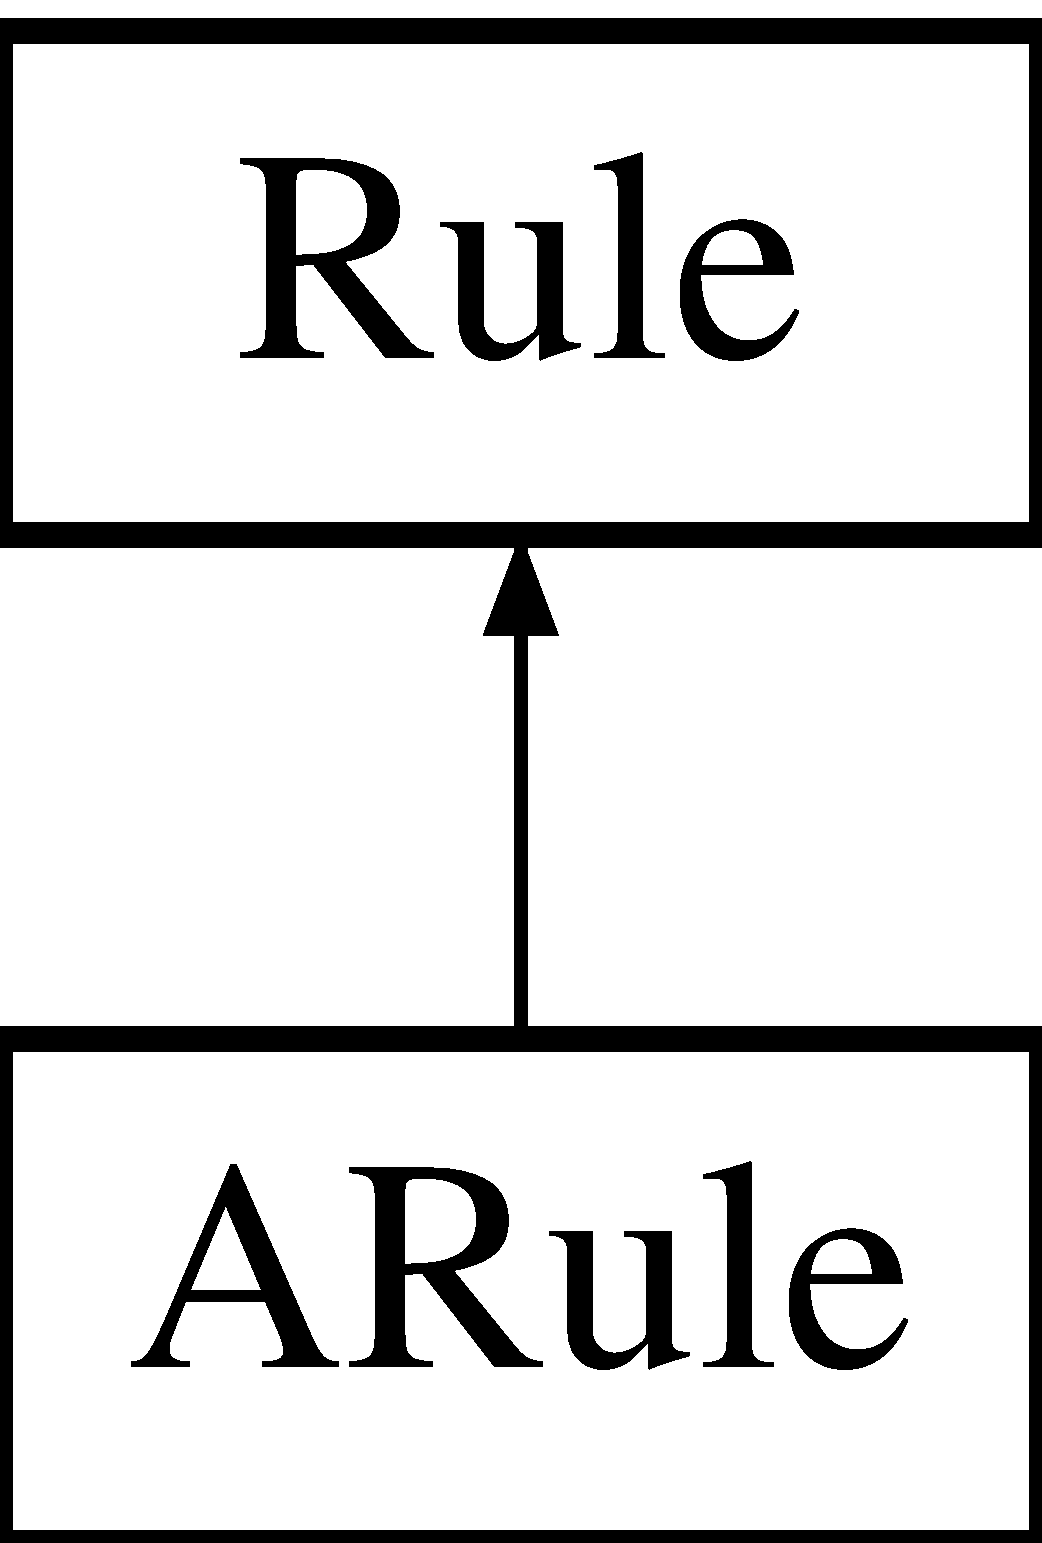
\includegraphics[height=2.000000cm]{class_d_t_r_1_1_a_rule}
\end{center}
\end{figure}
\subsection*{Additional Inherited Members}


\subsection{Detailed Description}
This class describes an asymmetrical rule.

An asymmetrical rule represents a two layers rule for which inverting layer1 and layer2 implies that the value of rule change. For example minimum enclosure rule is assymetrical.

Typical arules are\+: {\itshape min\+Extension, min\+Enclosure, min\+Length\+Enclosure, min\+Width\+Enclosure, line\+Extension, min\+Gate\+Extension, min\+Gate\+Enclosure} 
\hypertarget{class_bloc}{}\section{Bloc Class Reference}
\label{class_bloc}\index{Bloc@{Bloc}}


\subsection{Detailed Description}
This class describes a bloc of the placement tree. 
\hypertarget{class_s_p_i_c_e_1_1_capacitor}{}\section{Capacitor Class Reference}
\label{class_s_p_i_c_e_1_1_capacitor}\index{Capacitor@{Capacitor}}
Inheritance diagram for Capacitor\+:\begin{figure}[H]
\begin{center}
\leavevmode
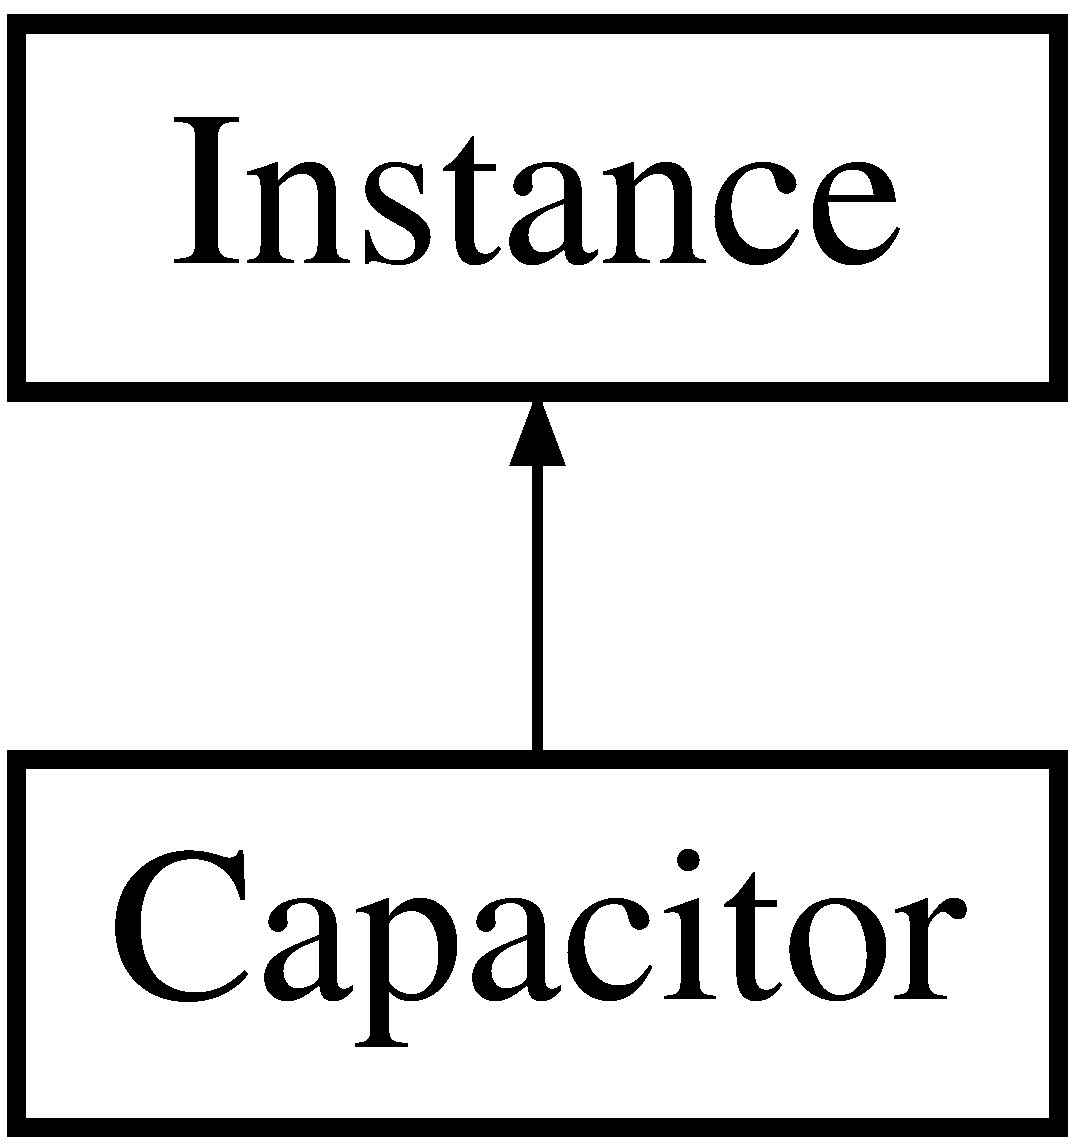
\includegraphics[height=2.000000cm]{class_s_p_i_c_e_1_1_capacitor}
\end{center}
\end{figure}
\subsection*{Public Member Functions}
\begin{DoxyCompactItemize}
\item 
\mbox{\hyperlink{class_s_p_i_c_e_1_1_capacitor_af3141143353c1a45fb2f2f35d3ddd28d}{Capacitor}} (std\+::string name, std\+::string pos, std\+::string neg, std\+::string value)
\begin{DoxyCompactList}\small\item\em creates a new capacitor. \end{DoxyCompactList}\item 
\mbox{\Hypertarget{class_s_p_i_c_e_1_1_capacitor_a8b4ab73ed1d99c533aa22af0a37ebb0d}\label{class_s_p_i_c_e_1_1_capacitor_a8b4ab73ed1d99c533aa22af0a37ebb0d}} 
std\+::string \mbox{\hyperlink{class_s_p_i_c_e_1_1_capacitor_a8b4ab73ed1d99c533aa22af0a37ebb0d}{get\+Negative}} ()
\begin{DoxyCompactList}\small\item\em returns the negative connector of the capacitor. \end{DoxyCompactList}\item 
\mbox{\Hypertarget{class_s_p_i_c_e_1_1_capacitor_a1adb347b9a2c2da556e4417ab0eec0e1}\label{class_s_p_i_c_e_1_1_capacitor_a1adb347b9a2c2da556e4417ab0eec0e1}} 
std\+::string \mbox{\hyperlink{class_s_p_i_c_e_1_1_capacitor_a1adb347b9a2c2da556e4417ab0eec0e1}{get\+Positive}} ()
\begin{DoxyCompactList}\small\item\em returns the positive connector of the capacitor. \end{DoxyCompactList}\item 
\mbox{\Hypertarget{class_s_p_i_c_e_1_1_capacitor_a4c052cb2622c580a250b2c783a436882}\label{class_s_p_i_c_e_1_1_capacitor_a4c052cb2622c580a250b2c783a436882}} 
std\+::string \mbox{\hyperlink{class_s_p_i_c_e_1_1_capacitor_a4c052cb2622c580a250b2c783a436882}{get\+Value}} ()
\begin{DoxyCompactList}\small\item\em returns the value of the capacitor. \end{DoxyCompactList}\end{DoxyCompactItemize}


\subsection{Detailed Description}
This class describes a capacitor which is a specialized instance which has a positive and a negative connector and a value. 

\subsection{Constructor \& Destructor Documentation}
\mbox{\Hypertarget{class_s_p_i_c_e_1_1_capacitor_af3141143353c1a45fb2f2f35d3ddd28d}\label{class_s_p_i_c_e_1_1_capacitor_af3141143353c1a45fb2f2f35d3ddd28d}} 
\index{S\+P\+I\+C\+E\+::\+Capacitor@{S\+P\+I\+C\+E\+::\+Capacitor}!Capacitor@{Capacitor}}
\index{Capacitor@{Capacitor}!S\+P\+I\+C\+E\+::\+Capacitor@{S\+P\+I\+C\+E\+::\+Capacitor}}
\subsubsection{\texorpdfstring{Capacitor()}{Capacitor()}}
{\footnotesize\ttfamily \mbox{\hyperlink{class_s_p_i_c_e_1_1_capacitor}{Capacitor}} (\begin{DoxyParamCaption}\item[{std\+::string}]{name,  }\item[{std\+::string}]{pos,  }\item[{std\+::string}]{neg,  }\item[{std\+::string}]{value }\end{DoxyParamCaption})\hspace{0.3cm}{\ttfamily [inline]}}



creates a new capacitor. 


\begin{DoxyParams}{Parameters}
{\em name} & the name of the capacitor. \\
\hline
{\em pos} & the positive connector of the capacitor. \\
\hline
{\em neg} & the negative connector of the capacitor. \\
\hline
{\em value} & the value of the capacitor. \\
\hline
\end{DoxyParams}

\hypertarget{class_c_i_f_1_1_circuit}{}\section{Circuit Class Reference}
\label{class_c_i_f_1_1_circuit}\index{Circuit@{Circuit}}
\subsection*{Public Member Functions}
\begin{DoxyCompactItemize}
\item 
bool \mbox{\hyperlink{class_c_i_f_1_1_circuit_a5b37e86206e2a128ba6db4987dc09a39}{add\+Polygon}} (\mbox{\hyperlink{class_c_i_f_1_1_polygon}{Polygon}} $\ast$)
\begin{DoxyCompactList}\small\item\em adds a \mbox{\hyperlink{class_c_i_f_1_1_polygon}{Polygon}} to the \mbox{\hyperlink{class_c_i_f_1_1_circuit}{Circuit}}. \end{DoxyCompactList}\item 
\mbox{\hyperlink{class_c_i_f_1_1_circuit_ad434e573e0ce37a59f39fa74fe9bfb79}{Circuit}} (std\+::string name, std\+::string unit, double scale)
\begin{DoxyCompactList}\small\item\em creates a new \mbox{\hyperlink{class_c_i_f_1_1_circuit}{Circuit}} \end{DoxyCompactList}\item 
bool \mbox{\hyperlink{class_c_i_f_1_1_circuit_a90c823b70c4984f302c19ceca604d101}{write\+To\+File}} (std\+::string)
\begin{DoxyCompactList}\small\item\em writes the database to file. \end{DoxyCompactList}\end{DoxyCompactItemize}


\subsection{Detailed Description}
This class contains all C\+IF circuit informations such as the name, the unit used, the scale and the list of all Polygons. 

\subsection{Constructor \& Destructor Documentation}
\mbox{\Hypertarget{class_c_i_f_1_1_circuit_ad434e573e0ce37a59f39fa74fe9bfb79}\label{class_c_i_f_1_1_circuit_ad434e573e0ce37a59f39fa74fe9bfb79}} 
\index{C\+I\+F\+::\+Circuit@{C\+I\+F\+::\+Circuit}!Circuit@{Circuit}}
\index{Circuit@{Circuit}!C\+I\+F\+::\+Circuit@{C\+I\+F\+::\+Circuit}}
\subsubsection{\texorpdfstring{Circuit()}{Circuit()}}
{\footnotesize\ttfamily \mbox{\hyperlink{class_c_i_f_1_1_circuit}{Circuit}} (\begin{DoxyParamCaption}\item[{std\+::string}]{name,  }\item[{std\+::string}]{unit,  }\item[{double}]{scale }\end{DoxyParamCaption})}



creates a new \mbox{\hyperlink{class_c_i_f_1_1_circuit}{Circuit}} 


\begin{DoxyParams}{Parameters}
{\em name} & the name of the circuit. \\
\hline
{\em unit} & the unit used for all distances \& coordinates. \\
\hline
{\em scale} & the scale used to convert DB unit to real unit (specified by the unit). \\
\hline
\end{DoxyParams}


\subsection{Member Function Documentation}
\mbox{\Hypertarget{class_c_i_f_1_1_circuit_a5b37e86206e2a128ba6db4987dc09a39}\label{class_c_i_f_1_1_circuit_a5b37e86206e2a128ba6db4987dc09a39}} 
\index{C\+I\+F\+::\+Circuit@{C\+I\+F\+::\+Circuit}!add\+Polygon@{add\+Polygon}}
\index{add\+Polygon@{add\+Polygon}!C\+I\+F\+::\+Circuit@{C\+I\+F\+::\+Circuit}}
\subsubsection{\texorpdfstring{add\+Polygon()}{addPolygon()}}
{\footnotesize\ttfamily bool add\+Polygon (\begin{DoxyParamCaption}\item[{\mbox{\hyperlink{class_c_i_f_1_1_polygon}{Polygon}} $\ast$}]{polygon }\end{DoxyParamCaption})}



adds a \mbox{\hyperlink{class_c_i_f_1_1_polygon}{Polygon}} to the \mbox{\hyperlink{class_c_i_f_1_1_circuit}{Circuit}}. 


\begin{DoxyParams}{Parameters}
{\em polygon} & the \mbox{\hyperlink{class_c_i_f_1_1_polygon}{Polygon}} object to add. \\
\hline
\end{DoxyParams}
\mbox{\Hypertarget{class_c_i_f_1_1_circuit_a90c823b70c4984f302c19ceca604d101}\label{class_c_i_f_1_1_circuit_a90c823b70c4984f302c19ceca604d101}} 
\index{C\+I\+F\+::\+Circuit@{C\+I\+F\+::\+Circuit}!write\+To\+File@{write\+To\+File}}
\index{write\+To\+File@{write\+To\+File}!C\+I\+F\+::\+Circuit@{C\+I\+F\+::\+Circuit}}
\subsubsection{\texorpdfstring{write\+To\+File()}{writeToFile()}}
{\footnotesize\ttfamily bool write\+To\+File (\begin{DoxyParamCaption}\item[{std\+::string}]{filename }\end{DoxyParamCaption})}



writes the database to file. 


\begin{DoxyParams}{Parameters}
{\em filename} & the destination file name.\\
\hline
\end{DoxyParams}
\begin{DoxyNote}{Note}
When driving file, current date and time are used to define date in generated C\+IF file. 
\end{DoxyNote}

\hypertarget{class_s_p_i_c_e_1_1_circuit}{}\section{Circuit Class Reference}
\label{class_s_p_i_c_e_1_1_circuit}\index{Circuit@{Circuit}}
\subsection*{Public Member Functions}
\begin{DoxyCompactItemize}
\item 
void \mbox{\hyperlink{class_s_p_i_c_e_1_1_circuit_a30fc53c4da54215fdec3ab1b96ea1943}{add\+Include}} (std\+::string)
\begin{DoxyCompactList}\small\item\em adds an include to the circuit. \end{DoxyCompactList}\item 
void \mbox{\hyperlink{class_s_p_i_c_e_1_1_circuit_a7bb4a4532643568ab1ac2c229185a88e}{add\+Instance}} (\mbox{\hyperlink{class_s_p_i_c_e_1_1_instance}{Instance}} $\ast$)
\begin{DoxyCompactList}\small\item\em adds an instance to the circuit. \end{DoxyCompactList}\item 
void \mbox{\hyperlink{class_s_p_i_c_e_1_1_circuit_a49939060cc1cb8e4bfaf003025032096}{add\+Library}} (std\+::string file, std\+::string type=\char`\"{}\char`\"{})
\begin{DoxyCompactList}\small\item\em adds a library to the circuit. \end{DoxyCompactList}\item 
void \mbox{\hyperlink{class_s_p_i_c_e_1_1_circuit_a1abe34b48e2b6e1834a143fdef159cb9}{add\+Option}} (std\+::string, std\+::string)
\begin{DoxyCompactList}\small\item\em adds an option to the circuit. \end{DoxyCompactList}\item 
void \mbox{\hyperlink{class_s_p_i_c_e_1_1_circuit_ab3ab147a16bc490ce96db905a4ca271c}{add\+Parameter}} (std\+::string, std\+::string)
\begin{DoxyCompactList}\small\item\em adds a parameter to the circuit. \end{DoxyCompactList}\item 
void \mbox{\hyperlink{class_s_p_i_c_e_1_1_circuit_a627cf18c2763bb59f3d7e5142873251c}{add\+Source}} (\mbox{\hyperlink{class_s_p_i_c_e_1_1_source}{Source}} $\ast$)
\begin{DoxyCompactList}\small\item\em adds a source to the circuit. \end{DoxyCompactList}\item 
\mbox{\hyperlink{class_s_p_i_c_e_1_1_subckt}{Subckt}} $\ast$ \mbox{\hyperlink{class_s_p_i_c_e_1_1_circuit_a0d1352e46d4537ce1e5f651de40e91a6}{add\+Subckt}} (std\+::string)
\begin{DoxyCompactList}\small\item\em adds a subcircuit to the circuit. \end{DoxyCompactList}\item 
\mbox{\Hypertarget{class_s_p_i_c_e_1_1_circuit_a2210ebc37eee536dbe9b44a89690256c}\label{class_s_p_i_c_e_1_1_circuit_a2210ebc37eee536dbe9b44a89690256c}} 
\mbox{\hyperlink{class_s_p_i_c_e_1_1_circuit_a2210ebc37eee536dbe9b44a89690256c}{Circuit}} ()
\begin{DoxyCompactList}\small\item\em creates a new circuit \end{DoxyCompactList}\item 
\mbox{\Hypertarget{class_s_p_i_c_e_1_1_circuit_a312beaf640e84589e6644820355c8ed6}\label{class_s_p_i_c_e_1_1_circuit_a312beaf640e84589e6644820355c8ed6}} 
const string\+\_\+vector \& \mbox{\hyperlink{class_s_p_i_c_e_1_1_circuit_a312beaf640e84589e6644820355c8ed6}{get\+Includes}} ()
\begin{DoxyCompactList}\small\item\em returns the includes of the circuit. \end{DoxyCompactList}\item 
\mbox{\Hypertarget{class_s_p_i_c_e_1_1_circuit_a8e6e58ffab876152a740092520c35d73}\label{class_s_p_i_c_e_1_1_circuit_a8e6e58ffab876152a740092520c35d73}} 
const std\+::vector$<$ \mbox{\hyperlink{class_s_p_i_c_e_1_1_instance}{Instance}} $\ast$ $>$ \& \mbox{\hyperlink{class_s_p_i_c_e_1_1_circuit_a8e6e58ffab876152a740092520c35d73}{get\+Instances}} ()
\begin{DoxyCompactList}\small\item\em returns the instances of the circuit. \end{DoxyCompactList}\item 
\mbox{\Hypertarget{class_s_p_i_c_e_1_1_circuit_a3e6a71a711e4796470f1a2a1dc42aef6}\label{class_s_p_i_c_e_1_1_circuit_a3e6a71a711e4796470f1a2a1dc42aef6}} 
const strpair\+\_\+vector \& \mbox{\hyperlink{class_s_p_i_c_e_1_1_circuit_a3e6a71a711e4796470f1a2a1dc42aef6}{get\+Libraries}} ()
\begin{DoxyCompactList}\small\item\em returns the libraries of the circuit. \end{DoxyCompactList}\item 
\mbox{\Hypertarget{class_s_p_i_c_e_1_1_circuit_a4ee11ef79ef893c5621e0e7d26a7f9a7}\label{class_s_p_i_c_e_1_1_circuit_a4ee11ef79ef893c5621e0e7d26a7f9a7}} 
const strings\+\_\+map \& \mbox{\hyperlink{class_s_p_i_c_e_1_1_circuit_a4ee11ef79ef893c5621e0e7d26a7f9a7}{get\+Options}} ()
\begin{DoxyCompactList}\small\item\em returns the options of the circuit. \end{DoxyCompactList}\item 
const strings\+\_\+map \& \mbox{\hyperlink{class_s_p_i_c_e_1_1_circuit_a4c46676f9ead2db537a0dd963b4f08f1}{get\+Parameters}} ()
\begin{DoxyCompactList}\small\item\em returns all circuit\textquotesingle{}s parameters. \end{DoxyCompactList}\item 
\mbox{\Hypertarget{class_s_p_i_c_e_1_1_circuit_ac18caa525ed386c44874ee643c88e27b}\label{class_s_p_i_c_e_1_1_circuit_ac18caa525ed386c44874ee643c88e27b}} 
const std\+::vector$<$ \mbox{\hyperlink{class_s_p_i_c_e_1_1_source}{Source}} $\ast$ $>$ \& \mbox{\hyperlink{class_s_p_i_c_e_1_1_circuit_ac18caa525ed386c44874ee643c88e27b}{get\+Sources}} ()
\begin{DoxyCompactList}\small\item\em returns the sources of the circuit. \end{DoxyCompactList}\item 
\mbox{\Hypertarget{class_s_p_i_c_e_1_1_circuit_adcc4ca0de68f8ee05f0d5db3b7604930}\label{class_s_p_i_c_e_1_1_circuit_adcc4ca0de68f8ee05f0d5db3b7604930}} 
const std\+::vector$<$ \mbox{\hyperlink{class_s_p_i_c_e_1_1_subckt}{Subckt}} $\ast$ $>$ \& \mbox{\hyperlink{class_s_p_i_c_e_1_1_circuit_adcc4ca0de68f8ee05f0d5db3b7604930}{get\+Subckts}} ()
\begin{DoxyCompactList}\small\item\em returns the subckts of the circuit. \end{DoxyCompactList}\item 
\mbox{\Hypertarget{class_s_p_i_c_e_1_1_circuit_ad19721dd878c04c854a72af12d785741}\label{class_s_p_i_c_e_1_1_circuit_ad19721dd878c04c854a72af12d785741}} 
std\+::string \mbox{\hyperlink{class_s_p_i_c_e_1_1_circuit_ad19721dd878c04c854a72af12d785741}{get\+Title}} ()
\begin{DoxyCompactList}\small\item\em returns the title of the circuit. \end{DoxyCompactList}\item 
void \mbox{\hyperlink{class_s_p_i_c_e_1_1_circuit_a798df9ebd558e22c85eeceb5202e3123}{set\+Title}} (std\+::string)
\begin{DoxyCompactList}\small\item\em sets the title of the circuit. \end{DoxyCompactList}\end{DoxyCompactItemize}
\subsection*{Static Public Member Functions}
\begin{DoxyCompactItemize}
\item 
static \mbox{\hyperlink{class_s_p_i_c_e_1_1_circuit}{Circuit}} $\ast$ \mbox{\hyperlink{class_s_p_i_c_e_1_1_circuit_aa8294fe7d9ceddb5653d08ecae3eaf36}{read\+From\+File}} (const std\+::string \&)
\begin{DoxyCompactList}\small\item\em creates and returns a \mbox{\hyperlink{class_s_p_i_c_e_1_1_circuit}{Circuit}} object based on a database source file. \end{DoxyCompactList}\end{DoxyCompactItemize}


\subsection{Detailed Description}
This class is the root class which means that having this object in hand allows to get/set any information contained in the Spice file parsed/drived. 

\subsection{Member Function Documentation}
\mbox{\Hypertarget{class_s_p_i_c_e_1_1_circuit_a30fc53c4da54215fdec3ab1b96ea1943}\label{class_s_p_i_c_e_1_1_circuit_a30fc53c4da54215fdec3ab1b96ea1943}} 
\index{S\+P\+I\+C\+E\+::\+Circuit@{S\+P\+I\+C\+E\+::\+Circuit}!add\+Include@{add\+Include}}
\index{add\+Include@{add\+Include}!S\+P\+I\+C\+E\+::\+Circuit@{S\+P\+I\+C\+E\+::\+Circuit}}
\subsubsection{\texorpdfstring{add\+Include()}{addInclude()}}
{\footnotesize\ttfamily void add\+Include (\begin{DoxyParamCaption}\item[{std\+::string}]{include }\end{DoxyParamCaption})\hspace{0.3cm}{\ttfamily [inline]}}



adds an include to the circuit. 


\begin{DoxyParams}{Parameters}
{\em include} & the include to add. \\
\hline
\end{DoxyParams}
\mbox{\Hypertarget{class_s_p_i_c_e_1_1_circuit_a7bb4a4532643568ab1ac2c229185a88e}\label{class_s_p_i_c_e_1_1_circuit_a7bb4a4532643568ab1ac2c229185a88e}} 
\index{S\+P\+I\+C\+E\+::\+Circuit@{S\+P\+I\+C\+E\+::\+Circuit}!add\+Instance@{add\+Instance}}
\index{add\+Instance@{add\+Instance}!S\+P\+I\+C\+E\+::\+Circuit@{S\+P\+I\+C\+E\+::\+Circuit}}
\subsubsection{\texorpdfstring{add\+Instance()}{addInstance()}}
{\footnotesize\ttfamily void add\+Instance (\begin{DoxyParamCaption}\item[{\mbox{\hyperlink{class_s_p_i_c_e_1_1_instance}{Instance}} $\ast$}]{instance }\end{DoxyParamCaption})\hspace{0.3cm}{\ttfamily [inline]}}



adds an instance to the circuit. 


\begin{DoxyParams}{Parameters}
{\em instance} & the instance to add. \\
\hline
\end{DoxyParams}
\mbox{\Hypertarget{class_s_p_i_c_e_1_1_circuit_a49939060cc1cb8e4bfaf003025032096}\label{class_s_p_i_c_e_1_1_circuit_a49939060cc1cb8e4bfaf003025032096}} 
\index{S\+P\+I\+C\+E\+::\+Circuit@{S\+P\+I\+C\+E\+::\+Circuit}!add\+Library@{add\+Library}}
\index{add\+Library@{add\+Library}!S\+P\+I\+C\+E\+::\+Circuit@{S\+P\+I\+C\+E\+::\+Circuit}}
\subsubsection{\texorpdfstring{add\+Library()}{addLibrary()}}
{\footnotesize\ttfamily void add\+Library (\begin{DoxyParamCaption}\item[{std\+::string}]{file,  }\item[{std\+::string}]{type = {\ttfamily \char`\"{}\char`\"{}} }\end{DoxyParamCaption})\hspace{0.3cm}{\ttfamily [inline]}}



adds a library to the circuit. 


\begin{DoxyParams}{Parameters}
{\em file} & the file describing the library to add. \\
\hline
{\em type} & the type if several exist in the same file (this argument is optionnal) \\
\hline
\end{DoxyParams}
\mbox{\Hypertarget{class_s_p_i_c_e_1_1_circuit_a1abe34b48e2b6e1834a143fdef159cb9}\label{class_s_p_i_c_e_1_1_circuit_a1abe34b48e2b6e1834a143fdef159cb9}} 
\index{S\+P\+I\+C\+E\+::\+Circuit@{S\+P\+I\+C\+E\+::\+Circuit}!add\+Option@{add\+Option}}
\index{add\+Option@{add\+Option}!S\+P\+I\+C\+E\+::\+Circuit@{S\+P\+I\+C\+E\+::\+Circuit}}
\subsubsection{\texorpdfstring{add\+Option()}{addOption()}}
{\footnotesize\ttfamily void add\+Option (\begin{DoxyParamCaption}\item[{std\+::string}]{name,  }\item[{std\+::string}]{value }\end{DoxyParamCaption})}



adds an option to the circuit. 


\begin{DoxyParams}{Parameters}
{\em name} & the name of the option. \\
\hline
{\em value} & the value of the option.\\
\hline
\end{DoxyParams}
\begin{DoxyNote}{Note}
The value is represented as a std\+::string to keep the optionnal unity. 
\end{DoxyNote}
\mbox{\Hypertarget{class_s_p_i_c_e_1_1_circuit_ab3ab147a16bc490ce96db905a4ca271c}\label{class_s_p_i_c_e_1_1_circuit_ab3ab147a16bc490ce96db905a4ca271c}} 
\index{S\+P\+I\+C\+E\+::\+Circuit@{S\+P\+I\+C\+E\+::\+Circuit}!add\+Parameter@{add\+Parameter}}
\index{add\+Parameter@{add\+Parameter}!S\+P\+I\+C\+E\+::\+Circuit@{S\+P\+I\+C\+E\+::\+Circuit}}
\subsubsection{\texorpdfstring{add\+Parameter()}{addParameter()}}
{\footnotesize\ttfamily void add\+Parameter (\begin{DoxyParamCaption}\item[{std\+::string}]{name,  }\item[{std\+::string}]{value }\end{DoxyParamCaption})\hspace{0.3cm}{\ttfamily [inline]}}



adds a parameter to the circuit. 

adds an equation parameter to the circuit.


\begin{DoxyParams}{Parameters}
{\em name} & the name of the parameter. \\
\hline
{\em value} & the value of the parameter.\\
\hline
{\em name} & the name of the parameter. \\
\hline
{\em equation} & the equation string of the parameter.\\
\hline
{\em name} & the name of the parameter. \\
\hline
{\em value} & the value of the parameter.\\
\hline
\end{DoxyParams}
\begin{DoxyNote}{Note}
The value is represented as a std\+::string to keep the optionnal unity. 
\end{DoxyNote}
\mbox{\Hypertarget{class_s_p_i_c_e_1_1_circuit_a627cf18c2763bb59f3d7e5142873251c}\label{class_s_p_i_c_e_1_1_circuit_a627cf18c2763bb59f3d7e5142873251c}} 
\index{S\+P\+I\+C\+E\+::\+Circuit@{S\+P\+I\+C\+E\+::\+Circuit}!add\+Source@{add\+Source}}
\index{add\+Source@{add\+Source}!S\+P\+I\+C\+E\+::\+Circuit@{S\+P\+I\+C\+E\+::\+Circuit}}
\subsubsection{\texorpdfstring{add\+Source()}{addSource()}}
{\footnotesize\ttfamily void add\+Source (\begin{DoxyParamCaption}\item[{\mbox{\hyperlink{class_s_p_i_c_e_1_1_source}{Source}} $\ast$}]{source }\end{DoxyParamCaption})\hspace{0.3cm}{\ttfamily [inline]}}



adds a source to the circuit. 


\begin{DoxyParams}{Parameters}
{\em source} & the source to add. \\
\hline
\end{DoxyParams}
\mbox{\Hypertarget{class_s_p_i_c_e_1_1_circuit_a0d1352e46d4537ce1e5f651de40e91a6}\label{class_s_p_i_c_e_1_1_circuit_a0d1352e46d4537ce1e5f651de40e91a6}} 
\index{S\+P\+I\+C\+E\+::\+Circuit@{S\+P\+I\+C\+E\+::\+Circuit}!add\+Subckt@{add\+Subckt}}
\index{add\+Subckt@{add\+Subckt}!S\+P\+I\+C\+E\+::\+Circuit@{S\+P\+I\+C\+E\+::\+Circuit}}
\subsubsection{\texorpdfstring{add\+Subckt()}{addSubckt()}}
{\footnotesize\ttfamily \mbox{\hyperlink{class_s_p_i_c_e_1_1_subckt}{Subckt}} $\ast$ add\+Subckt (\begin{DoxyParamCaption}\item[{std\+::string}]{name }\end{DoxyParamCaption})}



adds a subcircuit to the circuit. 


\begin{DoxyParams}{Parameters}
{\em name} & the name of the subckt.\\
\hline
\end{DoxyParams}
\begin{DoxyReturn}{Returns}
the newly created \mbox{\hyperlink{class_s_p_i_c_e_1_1_subckt}{Subckt}}. 
\end{DoxyReturn}
\mbox{\Hypertarget{class_s_p_i_c_e_1_1_circuit_a4c46676f9ead2db537a0dd963b4f08f1}\label{class_s_p_i_c_e_1_1_circuit_a4c46676f9ead2db537a0dd963b4f08f1}} 
\index{S\+P\+I\+C\+E\+::\+Circuit@{S\+P\+I\+C\+E\+::\+Circuit}!get\+Parameters@{get\+Parameters}}
\index{get\+Parameters@{get\+Parameters}!S\+P\+I\+C\+E\+::\+Circuit@{S\+P\+I\+C\+E\+::\+Circuit}}
\subsubsection{\texorpdfstring{get\+Parameters()}{getParameters()}}
{\footnotesize\ttfamily const Circuit\+::strings\+\_\+map \& get\+Parameters (\begin{DoxyParamCaption}{ }\end{DoxyParamCaption})\hspace{0.3cm}{\ttfamily [inline]}}



returns all circuit\textquotesingle{}s parameters. 

returns the parameters of the circuit. \mbox{\Hypertarget{class_s_p_i_c_e_1_1_circuit_aa8294fe7d9ceddb5653d08ecae3eaf36}\label{class_s_p_i_c_e_1_1_circuit_aa8294fe7d9ceddb5653d08ecae3eaf36}} 
\index{S\+P\+I\+C\+E\+::\+Circuit@{S\+P\+I\+C\+E\+::\+Circuit}!read\+From\+File@{read\+From\+File}}
\index{read\+From\+File@{read\+From\+File}!S\+P\+I\+C\+E\+::\+Circuit@{S\+P\+I\+C\+E\+::\+Circuit}}
\subsubsection{\texorpdfstring{read\+From\+File()}{readFromFile()}}
{\footnotesize\ttfamily \mbox{\hyperlink{class_s_p_i_c_e_1_1_circuit}{Circuit}} $\ast$ read\+From\+File (\begin{DoxyParamCaption}\item[{const std\+::string \&}]{filename }\end{DoxyParamCaption})\hspace{0.3cm}{\ttfamily [static]}}



creates and returns a \mbox{\hyperlink{class_s_p_i_c_e_1_1_circuit}{Circuit}} object based on a database source file. 


\begin{DoxyParams}{Parameters}
{\em file\+Path} & the source file name.\\
\hline
\end{DoxyParams}
\begin{DoxyReturn}{Returns}
the newly created \mbox{\hyperlink{class_s_p_i_c_e_1_1_circuit}{Circuit}}. 
\end{DoxyReturn}
\mbox{\Hypertarget{class_s_p_i_c_e_1_1_circuit_a798df9ebd558e22c85eeceb5202e3123}\label{class_s_p_i_c_e_1_1_circuit_a798df9ebd558e22c85eeceb5202e3123}} 
\index{S\+P\+I\+C\+E\+::\+Circuit@{S\+P\+I\+C\+E\+::\+Circuit}!set\+Title@{set\+Title}}
\index{set\+Title@{set\+Title}!S\+P\+I\+C\+E\+::\+Circuit@{S\+P\+I\+C\+E\+::\+Circuit}}
\subsubsection{\texorpdfstring{set\+Title()}{setTitle()}}
{\footnotesize\ttfamily void set\+Title (\begin{DoxyParamCaption}\item[{std\+::string}]{title }\end{DoxyParamCaption})\hspace{0.3cm}{\ttfamily [inline]}}



sets the title of the circuit. 


\begin{DoxyParams}{Parameters}
{\em title} & the title of the circuit \\
\hline
\end{DoxyParams}

\hypertarget{class_circuit}{}\section{Circuit Class Reference}
\label{class_circuit}\index{Circuit@{Circuit}}


\subsection{Detailed Description}
This class is the root class whihch means that having this object in hand allows to get/set any information contained in the Open\+Chams file parsed/drived. 
\hypertarget{class_net_1_1_connection}{}\section{Net\+:\+:Connection Class Reference}
\label{class_net_1_1_connection}\index{Net\+::\+Connection@{Net\+::\+Connection}}


\subsection{Detailed Description}
This class describe a \mbox{\hyperlink{class_net_1_1_connection}{Connection}} in a \mbox{\hyperlink{class_net}{Net}}. A connection is a couple (instance\+Name, connector\+Name) used to represent all the connectors linked to a net. 
\hypertarget{class_operator_1_1_constraint}{}\section{Operator\+:\+:Constraint Class Reference}
\label{class_operator_1_1_constraint}\index{Operator\+::\+Constraint@{Operator\+::\+Constraint}}


\subsection{Detailed Description}
This class describes a constraint. A constraint is used to set that a parameter\textquotesingle{}s value is defined relative to another parameter value or to an equation\+: device\+A.\+paramI = device\+B.\+paramJ $\ast$ factor device\+A.\+paramI = equation $\ast$ factor 
\hypertarget{class_s_p_i_c_e_1_1_current}{}\section{Current Class Reference}
\label{class_s_p_i_c_e_1_1_current}\index{Current@{Current}}
Inheritance diagram for Current\+:\begin{figure}[H]
\begin{center}
\leavevmode
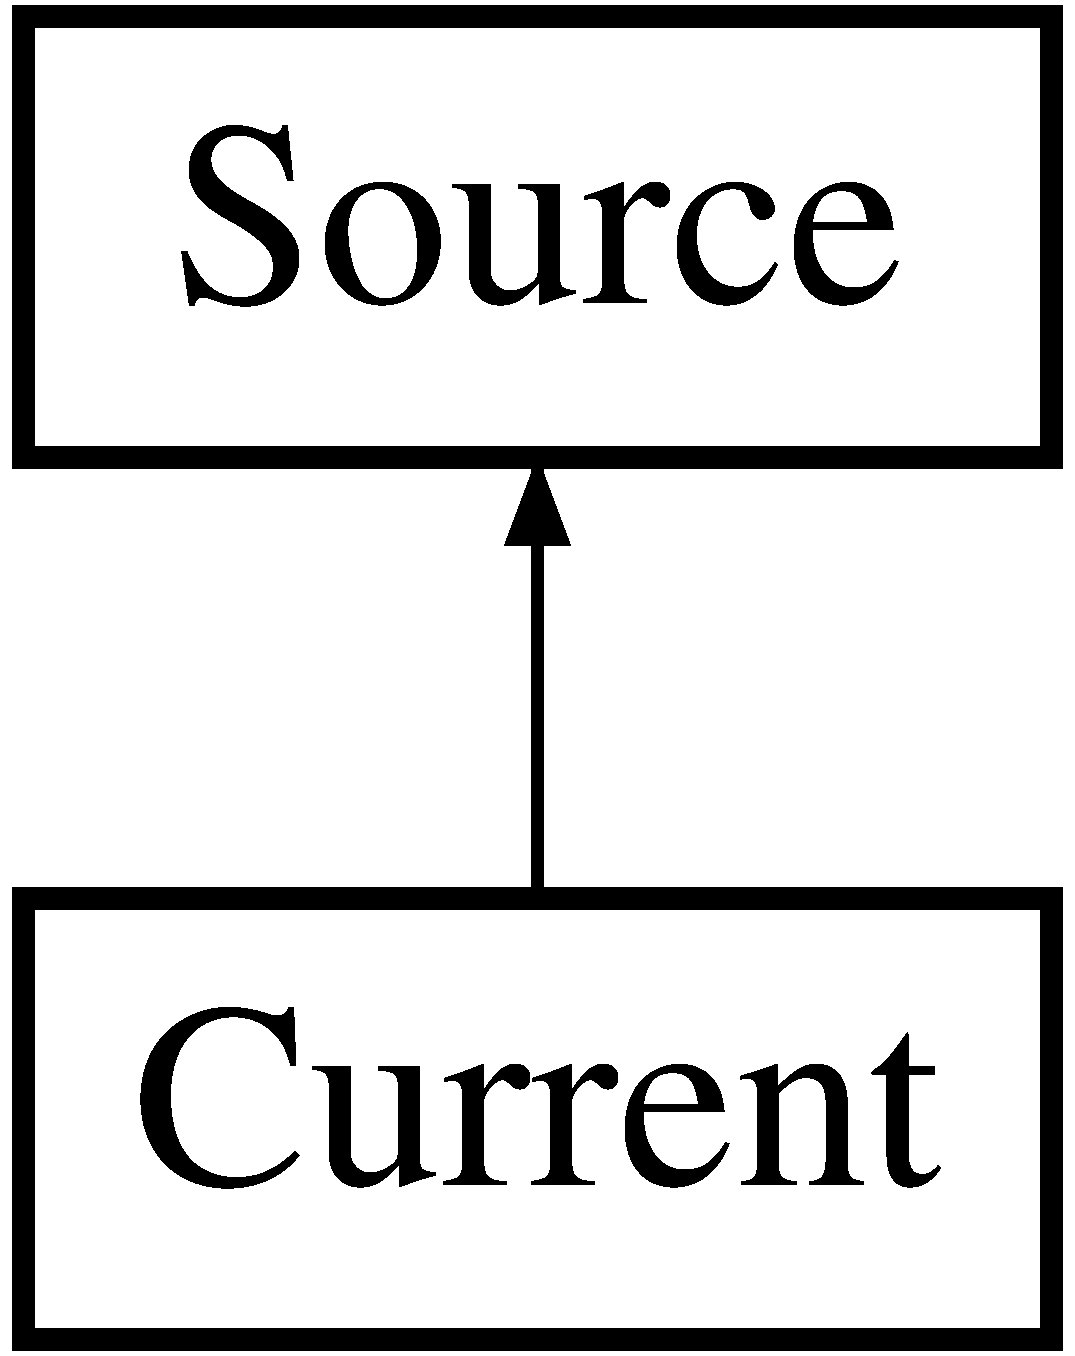
\includegraphics[height=2.000000cm]{class_s_p_i_c_e_1_1_current}
\end{center}
\end{figure}
\subsection*{Public Member Functions}
\begin{DoxyCompactItemize}
\item 
\mbox{\hyperlink{class_s_p_i_c_e_1_1_current_a798deca3f9017adbf1bb2ab5ca2f2f5e}{Current}} (std\+::string name, std\+::string pos, std\+::string neg, std\+::string value)
\begin{DoxyCompactList}\small\item\em creates a new current source. \end{DoxyCompactList}\end{DoxyCompactItemize}
\subsection*{Additional Inherited Members}


\subsection{Detailed Description}
This class describes a current source. 

\subsection{Constructor \& Destructor Documentation}
\mbox{\Hypertarget{class_s_p_i_c_e_1_1_current_a798deca3f9017adbf1bb2ab5ca2f2f5e}\label{class_s_p_i_c_e_1_1_current_a798deca3f9017adbf1bb2ab5ca2f2f5e}} 
\index{S\+P\+I\+C\+E\+::\+Current@{S\+P\+I\+C\+E\+::\+Current}!Current@{Current}}
\index{Current@{Current}!S\+P\+I\+C\+E\+::\+Current@{S\+P\+I\+C\+E\+::\+Current}}
\subsubsection{\texorpdfstring{Current()}{Current()}}
{\footnotesize\ttfamily \mbox{\hyperlink{class_s_p_i_c_e_1_1_current}{Current}} (\begin{DoxyParamCaption}\item[{std\+::string}]{name,  }\item[{std\+::string}]{pos,  }\item[{std\+::string}]{neg,  }\item[{std\+::string}]{value }\end{DoxyParamCaption})\hspace{0.3cm}{\ttfamily [inline]}}



creates a new current source. 


\begin{DoxyParams}{Parameters}
{\em name} & the name of the source. \\
\hline
{\em pos} & the positive connector of the source. \\
\hline
{\em neg} & the negative connector of the source. \\
\hline
{\em value} & the value of the source. \\
\hline
\end{DoxyParams}

\hypertarget{class_device}{}\section{Device Class Reference}
\label{class_device}\index{Device@{Device}}


\subsection{Detailed Description}
This class describes a \mbox{\hyperlink{class_device}{Device}}.

A device is a leaf instance which means its model is not defined in a external file but is described inside the device. As an instance, the \mbox{\hyperlink{class_device}{Device}} inherits all \mbox{\hyperlink{class_instance}{Instance}} methods and adds specific properties\+: mos type, bulk connection and list of internal transistors.

\begin{DoxyNote}{Note}
Althought today \mbox{\hyperlink{class_device}{Device}} object only consider Transistor\+Family devices, it will have to consider other devices, such as Capacitor when C\+H\+A\+MS project will. 
\end{DoxyNote}

\hypertarget{class_d_t_r_1_1_d_t_r_exception}{}\section{D\+T\+R\+Exception Class Reference}
\label{class_d_t_r_1_1_d_t_r_exception}\index{D\+T\+R\+Exception@{D\+T\+R\+Exception}}


\subsection{Detailed Description}
This class describes the exceptions throwed by the D\+TR library in case of errors. 
\hypertarget{class_a_g_d_s_1_1_element}{}\section{Element Class Reference}
\label{class_a_g_d_s_1_1_element}\index{Element@{Element}}
Inheritance diagram for Element\+:\begin{figure}[H]
\begin{center}
\leavevmode
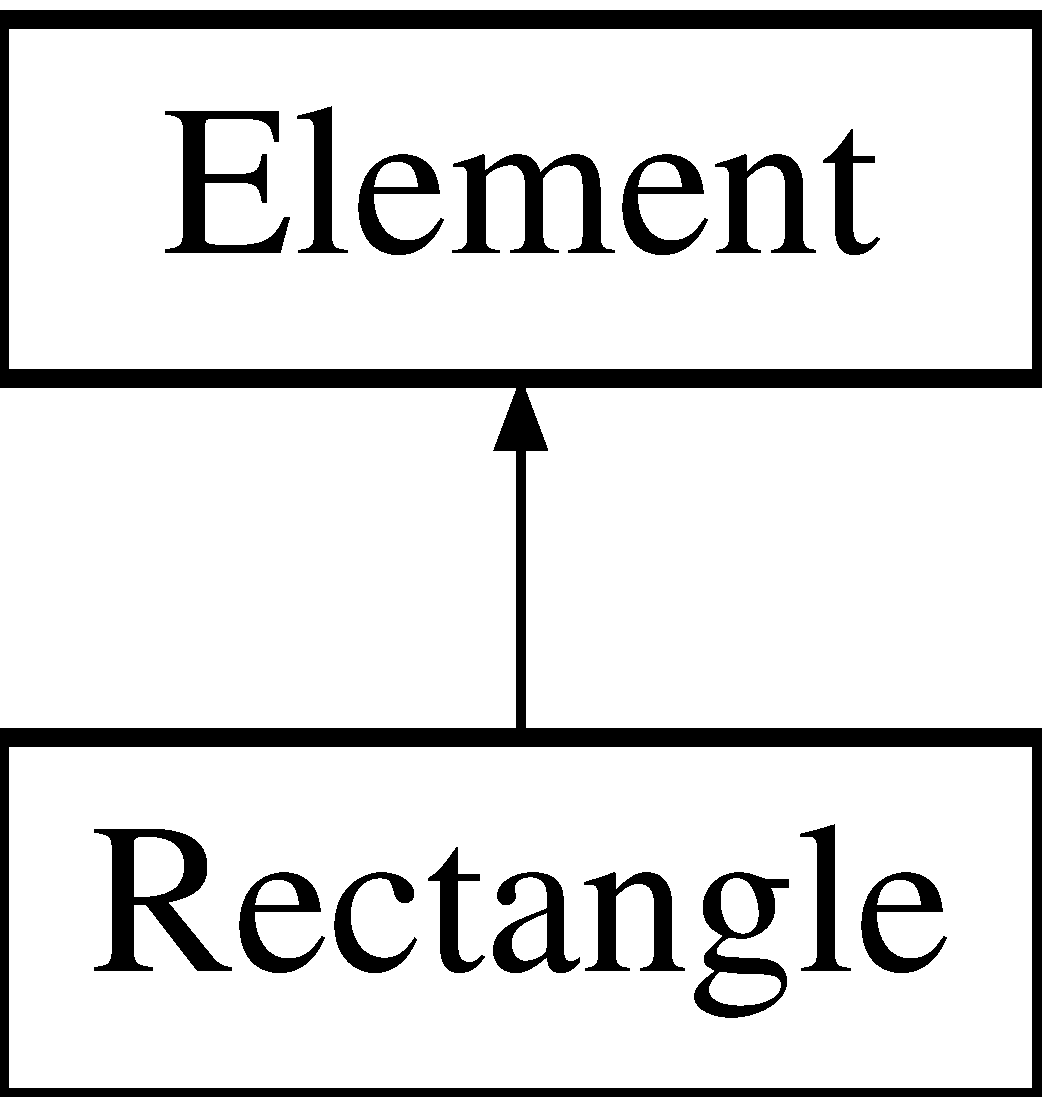
\includegraphics[height=2.000000cm]{class_a_g_d_s_1_1_element}
\end{center}
\end{figure}


\subsection{Detailed Description}
This is an abstract class which is a base for any G\+DS II shape. It only defines a layer. 
\hypertarget{class_group}{}\section{Group Class Reference}
\label{class_group}\index{Group@{Group}}


\subsection{Detailed Description}
This class describes a group of the placement tree. 
\hypertarget{class_schematic_1_1_infos}{}\section{Schematic\+:\+:Infos Class Reference}
\label{class_schematic_1_1_infos}\index{Schematic\+::\+Infos@{Schematic\+::\+Infos}}


\subsection{Detailed Description}
This class describes schematic informations for an instance. It contains x and y coordinates and the orientation of the instance. 
\hypertarget{class_s_p_i_c_e_1_1_instance}{}\section{Instance Class Reference}
\label{class_s_p_i_c_e_1_1_instance}\index{Instance@{Instance}}
Inheritance diagram for Instance\+:\begin{figure}[H]
\begin{center}
\leavevmode
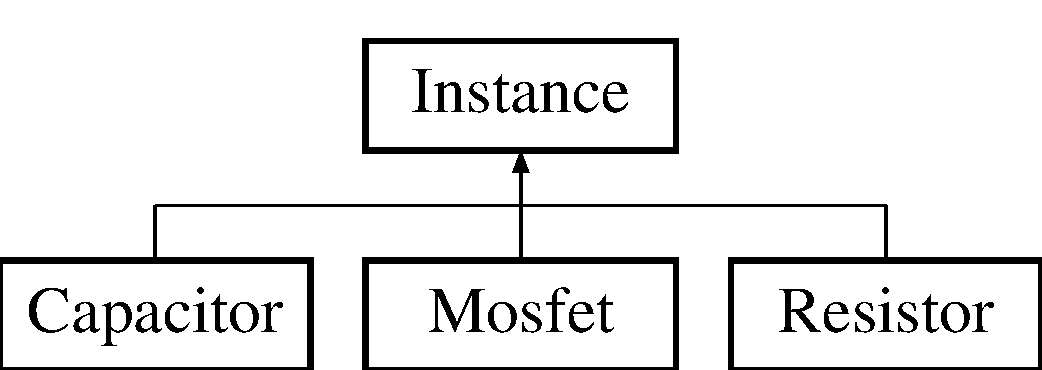
\includegraphics[height=2.000000cm]{class_s_p_i_c_e_1_1_instance}
\end{center}
\end{figure}
\subsection*{Public Member Functions}
\begin{DoxyCompactItemize}
\item 
void \mbox{\hyperlink{class_s_p_i_c_e_1_1_instance_af9aeca34e780851a2b024df7c5ff5b54}{add\+Connector}} (std\+::string connector)
\begin{DoxyCompactList}\small\item\em adds a connector to the instance. \end{DoxyCompactList}\item 
void \mbox{\hyperlink{class_s_p_i_c_e_1_1_instance_a8d69bbbea5ece0949e100c464e412f20}{add\+Parameter}} (std\+::string name, std\+::string value)
\begin{DoxyCompactList}\small\item\em adds a parameter to the instance. \end{DoxyCompactList}\item 
const std\+::vector$<$ std\+::string $>$ \& \mbox{\hyperlink{class_s_p_i_c_e_1_1_instance_acce8940edeaa3d79c522006f987e0711}{get\+Connectors}} ()
\begin{DoxyCompactList}\small\item\em returns the map of instance\textquotesingle{}s connectors. \end{DoxyCompactList}\item 
\mbox{\Hypertarget{class_s_p_i_c_e_1_1_instance_afc74cbe93df9c473a53db83a325f8f9d}\label{class_s_p_i_c_e_1_1_instance_afc74cbe93df9c473a53db83a325f8f9d}} 
std\+::string \mbox{\hyperlink{class_s_p_i_c_e_1_1_instance_afc74cbe93df9c473a53db83a325f8f9d}{get\+Model}} ()
\begin{DoxyCompactList}\small\item\em returns the model of the instance. \end{DoxyCompactList}\item 
\mbox{\Hypertarget{class_s_p_i_c_e_1_1_instance_ac0fc966d4386ddb71d99361e3fccb311}\label{class_s_p_i_c_e_1_1_instance_ac0fc966d4386ddb71d99361e3fccb311}} 
std\+::string \mbox{\hyperlink{class_s_p_i_c_e_1_1_instance_ac0fc966d4386ddb71d99361e3fccb311}{get\+Name}} ()
\begin{DoxyCompactList}\small\item\em returns the name of the instance. \end{DoxyCompactList}\item 
\mbox{\Hypertarget{class_s_p_i_c_e_1_1_instance_aee7d59083b78d31ac5c19ab508da91e0}\label{class_s_p_i_c_e_1_1_instance_aee7d59083b78d31ac5c19ab508da91e0}} 
const std\+::map$<$ std\+::string, std\+::string $>$ \& \mbox{\hyperlink{class_s_p_i_c_e_1_1_instance_aee7d59083b78d31ac5c19ab508da91e0}{get\+Parameters}} ()
\begin{DoxyCompactList}\small\item\em returns the parameters of the instance. \end{DoxyCompactList}\item 
std\+::string \mbox{\hyperlink{class_s_p_i_c_e_1_1_instance_a324e4ff99afdcd5972d8c57461d12ef5}{get\+Parameter\+Value}} (std\+::string name)
\begin{DoxyCompactList}\small\item\em returns the value (as string) of a parameter of the instance. \end{DoxyCompactList}\item 
\mbox{\hyperlink{class_s_p_i_c_e_1_1_instance_a400232cdfbe82c01dd2830368377492b}{Instance}} (std\+::string name, std\+::string model)
\begin{DoxyCompactList}\small\item\em creates a new instance. \end{DoxyCompactList}\end{DoxyCompactItemize}


\subsection{Detailed Description}
This class describes an instance of the global circuit. It is the base class of \mbox{\hyperlink{class_s_p_i_c_e_1_1_capacitor}{S\+P\+I\+C\+E\+::\+Capacitor}}, \mbox{\hyperlink{class_s_p_i_c_e_1_1_mosfet}{S\+P\+I\+C\+E\+::\+Mosfet}} and \mbox{\hyperlink{class_s_p_i_c_e_1_1_resistor}{S\+P\+I\+C\+E\+::\+Resistor}}. 

\subsection{Constructor \& Destructor Documentation}
\mbox{\Hypertarget{class_s_p_i_c_e_1_1_instance_a400232cdfbe82c01dd2830368377492b}\label{class_s_p_i_c_e_1_1_instance_a400232cdfbe82c01dd2830368377492b}} 
\index{S\+P\+I\+C\+E\+::\+Instance@{S\+P\+I\+C\+E\+::\+Instance}!Instance@{Instance}}
\index{Instance@{Instance}!S\+P\+I\+C\+E\+::\+Instance@{S\+P\+I\+C\+E\+::\+Instance}}
\subsubsection{\texorpdfstring{Instance()}{Instance()}}
{\footnotesize\ttfamily \mbox{\hyperlink{class_s_p_i_c_e_1_1_instance}{Instance}} (\begin{DoxyParamCaption}\item[{std\+::string}]{name,  }\item[{std\+::string}]{model }\end{DoxyParamCaption})}



creates a new instance. 


\begin{DoxyParams}{Parameters}
{\em name} & the name of the instance. \\
\hline
{\em model} & the model of the instance. \\
\hline
{\em netlist} & the netlist to which the instance belongs.\\
\hline
{\em name} & the name of the instance. \\
\hline
{\em model} & the model of the instance. \\
\hline
\end{DoxyParams}


\subsection{Member Function Documentation}
\mbox{\Hypertarget{class_s_p_i_c_e_1_1_instance_af9aeca34e780851a2b024df7c5ff5b54}\label{class_s_p_i_c_e_1_1_instance_af9aeca34e780851a2b024df7c5ff5b54}} 
\index{S\+P\+I\+C\+E\+::\+Instance@{S\+P\+I\+C\+E\+::\+Instance}!add\+Connector@{add\+Connector}}
\index{add\+Connector@{add\+Connector}!S\+P\+I\+C\+E\+::\+Instance@{S\+P\+I\+C\+E\+::\+Instance}}
\subsubsection{\texorpdfstring{add\+Connector()}{addConnector()}}
{\footnotesize\ttfamily void add\+Connector (\begin{DoxyParamCaption}\item[{std\+::string}]{connector }\end{DoxyParamCaption})\hspace{0.3cm}{\ttfamily [inline]}}



adds a connector to the instance. 


\begin{DoxyParams}{Parameters}
{\em name} & the name of the connector.\\
\hline
{\em connector} & the connector to add. \\
\hline
\end{DoxyParams}
\mbox{\Hypertarget{class_s_p_i_c_e_1_1_instance_a8d69bbbea5ece0949e100c464e412f20}\label{class_s_p_i_c_e_1_1_instance_a8d69bbbea5ece0949e100c464e412f20}} 
\index{S\+P\+I\+C\+E\+::\+Instance@{S\+P\+I\+C\+E\+::\+Instance}!add\+Parameter@{add\+Parameter}}
\index{add\+Parameter@{add\+Parameter}!S\+P\+I\+C\+E\+::\+Instance@{S\+P\+I\+C\+E\+::\+Instance}}
\subsubsection{\texorpdfstring{add\+Parameter()}{addParameter()}}
{\footnotesize\ttfamily void add\+Parameter (\begin{DoxyParamCaption}\item[{std\+::string}]{name,  }\item[{std\+::string}]{value }\end{DoxyParamCaption})\hspace{0.3cm}{\ttfamily [inline]}}



adds a parameter to the instance. 

add a parameter to the instance.

adds an equation parameter to the instance.


\begin{DoxyParams}{Parameters}
{\em name} & the name of the parameter. \\
\hline
{\em value} & the value of the parameter.\\
\hline
{\em name} & the name of the parameter. \\
\hline
{\em equation} & the equation string of the parameter. \\
\hline
\end{DoxyParams}
\mbox{\Hypertarget{class_s_p_i_c_e_1_1_instance_acce8940edeaa3d79c522006f987e0711}\label{class_s_p_i_c_e_1_1_instance_acce8940edeaa3d79c522006f987e0711}} 
\index{S\+P\+I\+C\+E\+::\+Instance@{S\+P\+I\+C\+E\+::\+Instance}!get\+Connectors@{get\+Connectors}}
\index{get\+Connectors@{get\+Connectors}!S\+P\+I\+C\+E\+::\+Instance@{S\+P\+I\+C\+E\+::\+Instance}}
\subsubsection{\texorpdfstring{get\+Connectors()}{getConnectors()}}
{\footnotesize\ttfamily const std\+::vector$<$ std\+::string $>$ \& get\+Connectors (\begin{DoxyParamCaption}{ }\end{DoxyParamCaption})\hspace{0.3cm}{\ttfamily [inline]}}



returns the map of instance\textquotesingle{}s connectors. 

returns the connectors of the instance. \mbox{\Hypertarget{class_s_p_i_c_e_1_1_instance_a324e4ff99afdcd5972d8c57461d12ef5}\label{class_s_p_i_c_e_1_1_instance_a324e4ff99afdcd5972d8c57461d12ef5}} 
\index{S\+P\+I\+C\+E\+::\+Instance@{S\+P\+I\+C\+E\+::\+Instance}!get\+Parameter\+Value@{get\+Parameter\+Value}}
\index{get\+Parameter\+Value@{get\+Parameter\+Value}!S\+P\+I\+C\+E\+::\+Instance@{S\+P\+I\+C\+E\+::\+Instance}}
\subsubsection{\texorpdfstring{get\+Parameter\+Value()}{getParameterValue()}}
{\footnotesize\ttfamily string get\+Parameter\+Value (\begin{DoxyParamCaption}\item[{std\+::string}]{name }\end{DoxyParamCaption})}



returns the value (as string) of a parameter of the instance. 


\begin{DoxyParams}{Parameters}
{\em name} & the name of the parameter from which to get value. \\
\hline
\end{DoxyParams}

\hypertarget{class_instance}{}\section{Instance Class Reference}
\label{class_instance}\index{Instance@{Instance}}


\subsection{Detailed Description}
This class describes an instance.

Basicaly an instance is a subcircuit of the current (top) circuit. 
\hypertarget{class_instance_point}{}\section{Instance\+Point Class Reference}
\label{class_instance_point}\index{Instance\+Point@{Instance\+Point}}


\subsection{Detailed Description}
This class describes a wire point associated to an instance\textquotesingle{}s connector. 
\hypertarget{class_intermediate_point}{}\section{Intermediate\+Point Class Reference}
\label{class_intermediate_point}\index{Intermediate\+Point@{Intermediate\+Point}}


\subsection{Detailed Description}
This class describes a wire point defined by its (x,y) coordinates. 
\hypertarget{class_layout}{}\section{Layout Class Reference}
\label{class_layout}\index{Layout@{Layout}}


\subsection{Detailed Description}
This class describes layout informations for an \mbox{\hyperlink{class_instance}{Instance}}.

The \mbox{\hyperlink{class_layout}{Layout}} object is used to store all informations relative to physical layout of the instance (such as the layout style).

\begin{DoxyNote}{Note}
The \mbox{\hyperlink{class_layout}{Layout}} object is optionnal in \mbox{\hyperlink{class_circuit}{Circuit}}. 
\end{DoxyNote}

\hypertarget{class_a_g_d_s_1_1_library}{}\section{Library Class Reference}
\label{class_a_g_d_s_1_1_library}\index{Library@{Library}}
\subsection*{Public Member Functions}
\begin{DoxyCompactItemize}
\item 
bool \mbox{\hyperlink{class_a_g_d_s_1_1_library_a93d333a20154e0b688ff3ff213039171}{add\+Structure}} (\mbox{\hyperlink{class_a_g_d_s_1_1_structure}{Structure}} $\ast$)
\begin{DoxyCompactList}\small\item\em adds a \mbox{\hyperlink{class_a_g_d_s_1_1_structure}{Structure}} to the \mbox{\hyperlink{class_a_g_d_s_1_1_library}{Library}}. \end{DoxyCompactList}\item 
\mbox{\hyperlink{class_a_g_d_s_1_1_library_a9244ebe2cc60781aaf25cf559ea2473a}{Library}} (std\+::string lib\+Name)
\begin{DoxyCompactList}\small\item\em creates a new \mbox{\hyperlink{class_a_g_d_s_1_1_library}{Library}} \end{DoxyCompactList}\item 
void \mbox{\hyperlink{class_a_g_d_s_1_1_library_a938acb6eb8d14aade9dba7331c75ff0a}{set\+Phys\+Units}} (double phys\+Units)
\begin{DoxyCompactList}\small\item\em sets the physical units. \end{DoxyCompactList}\item 
void \mbox{\hyperlink{class_a_g_d_s_1_1_library_a0d0e972bb142f892c462bb8d7f04a50b}{set\+User\+Units}} (double user\+Units)
\begin{DoxyCompactList}\small\item\em sets the user units. \end{DoxyCompactList}\item 
bool \mbox{\hyperlink{class_a_g_d_s_1_1_library_a33b9d989b84857f46034085664ff3fa2}{write\+To\+File}} (std\+::string file\+Name)
\begin{DoxyCompactList}\small\item\em writes the database to file. \end{DoxyCompactList}\end{DoxyCompactItemize}


\subsection{Detailed Description}
This class contains all A\+G\+DS library informations such as the name, the unit used (user and physical) and the list of all Structures. 

\subsection{Constructor \& Destructor Documentation}
\mbox{\Hypertarget{class_a_g_d_s_1_1_library_a9244ebe2cc60781aaf25cf559ea2473a}\label{class_a_g_d_s_1_1_library_a9244ebe2cc60781aaf25cf559ea2473a}} 
\index{A\+G\+D\+S\+::\+Library@{A\+G\+D\+S\+::\+Library}!Library@{Library}}
\index{Library@{Library}!A\+G\+D\+S\+::\+Library@{A\+G\+D\+S\+::\+Library}}
\subsubsection{\texorpdfstring{Library()}{Library()}}
{\footnotesize\ttfamily \mbox{\hyperlink{class_a_g_d_s_1_1_library}{Library}} (\begin{DoxyParamCaption}\item[{std\+::string}]{name }\end{DoxyParamCaption})}



creates a new \mbox{\hyperlink{class_a_g_d_s_1_1_library}{Library}} 


\begin{DoxyParams}{Parameters}
{\em name} & the name of the library. \\
\hline
\end{DoxyParams}


\subsection{Member Function Documentation}
\mbox{\Hypertarget{class_a_g_d_s_1_1_library_a93d333a20154e0b688ff3ff213039171}\label{class_a_g_d_s_1_1_library_a93d333a20154e0b688ff3ff213039171}} 
\index{A\+G\+D\+S\+::\+Library@{A\+G\+D\+S\+::\+Library}!add\+Structure@{add\+Structure}}
\index{add\+Structure@{add\+Structure}!A\+G\+D\+S\+::\+Library@{A\+G\+D\+S\+::\+Library}}
\subsubsection{\texorpdfstring{add\+Structure()}{addStructure()}}
{\footnotesize\ttfamily bool add\+Structure (\begin{DoxyParamCaption}\item[{\mbox{\hyperlink{class_a_g_d_s_1_1_structure}{Structure}} $\ast$}]{str }\end{DoxyParamCaption})}



adds a \mbox{\hyperlink{class_a_g_d_s_1_1_structure}{Structure}} to the \mbox{\hyperlink{class_a_g_d_s_1_1_library}{Library}}. 


\begin{DoxyParams}{Parameters}
{\em str} & the \mbox{\hyperlink{class_a_g_d_s_1_1_structure}{Structure}} object to add. \\
\hline
\end{DoxyParams}
\mbox{\Hypertarget{class_a_g_d_s_1_1_library_a938acb6eb8d14aade9dba7331c75ff0a}\label{class_a_g_d_s_1_1_library_a938acb6eb8d14aade9dba7331c75ff0a}} 
\index{A\+G\+D\+S\+::\+Library@{A\+G\+D\+S\+::\+Library}!set\+Phys\+Units@{set\+Phys\+Units}}
\index{set\+Phys\+Units@{set\+Phys\+Units}!A\+G\+D\+S\+::\+Library@{A\+G\+D\+S\+::\+Library}}
\subsubsection{\texorpdfstring{set\+Phys\+Units()}{setPhysUnits()}}
{\footnotesize\ttfamily void set\+Phys\+Units (\begin{DoxyParamCaption}\item[{double}]{phys\+Units }\end{DoxyParamCaption})\hspace{0.3cm}{\ttfamily [inline]}}



sets the physical units. 


\begin{DoxyParams}{Parameters}
{\em phys\+Units} & the value of the physical units. \\
\hline
\end{DoxyParams}
\mbox{\Hypertarget{class_a_g_d_s_1_1_library_a0d0e972bb142f892c462bb8d7f04a50b}\label{class_a_g_d_s_1_1_library_a0d0e972bb142f892c462bb8d7f04a50b}} 
\index{A\+G\+D\+S\+::\+Library@{A\+G\+D\+S\+::\+Library}!set\+User\+Units@{set\+User\+Units}}
\index{set\+User\+Units@{set\+User\+Units}!A\+G\+D\+S\+::\+Library@{A\+G\+D\+S\+::\+Library}}
\subsubsection{\texorpdfstring{set\+User\+Units()}{setUserUnits()}}
{\footnotesize\ttfamily void set\+User\+Units (\begin{DoxyParamCaption}\item[{double}]{user\+Units }\end{DoxyParamCaption})\hspace{0.3cm}{\ttfamily [inline]}}



sets the user units. 


\begin{DoxyParams}{Parameters}
{\em user\+Units} & the value of the user units. \\
\hline
\end{DoxyParams}
\mbox{\Hypertarget{class_a_g_d_s_1_1_library_a33b9d989b84857f46034085664ff3fa2}\label{class_a_g_d_s_1_1_library_a33b9d989b84857f46034085664ff3fa2}} 
\index{A\+G\+D\+S\+::\+Library@{A\+G\+D\+S\+::\+Library}!write\+To\+File@{write\+To\+File}}
\index{write\+To\+File@{write\+To\+File}!A\+G\+D\+S\+::\+Library@{A\+G\+D\+S\+::\+Library}}
\subsubsection{\texorpdfstring{write\+To\+File()}{writeToFile()}}
{\footnotesize\ttfamily bool write\+To\+File (\begin{DoxyParamCaption}\item[{std\+::string}]{filename }\end{DoxyParamCaption})}



writes the database to file. 


\begin{DoxyParams}{Parameters}
{\em filename} & the destination file name.\\
\hline
\end{DoxyParams}
\begin{DoxyNote}{Note}
When driving file, current date and time are used to define date in generated C\+IF file. 
\end{DoxyNote}

\hypertarget{struct_s_p_i_c_e_1_1map__item}{}\section{map\+\_\+item$<$ Key, Val $>$ Struct Template Reference}
\label{struct_s_p_i_c_e_1_1map__item}\index{map\+\_\+item$<$ Key, Val $>$@{map\+\_\+item$<$ Key, Val $>$}}

\hypertarget{class_s_p_i_c_e_1_1_mosfet}{}\section{Mosfet Class Reference}
\label{class_s_p_i_c_e_1_1_mosfet}\index{Mosfet@{Mosfet}}
Inheritance diagram for Mosfet\+:\begin{figure}[H]
\begin{center}
\leavevmode
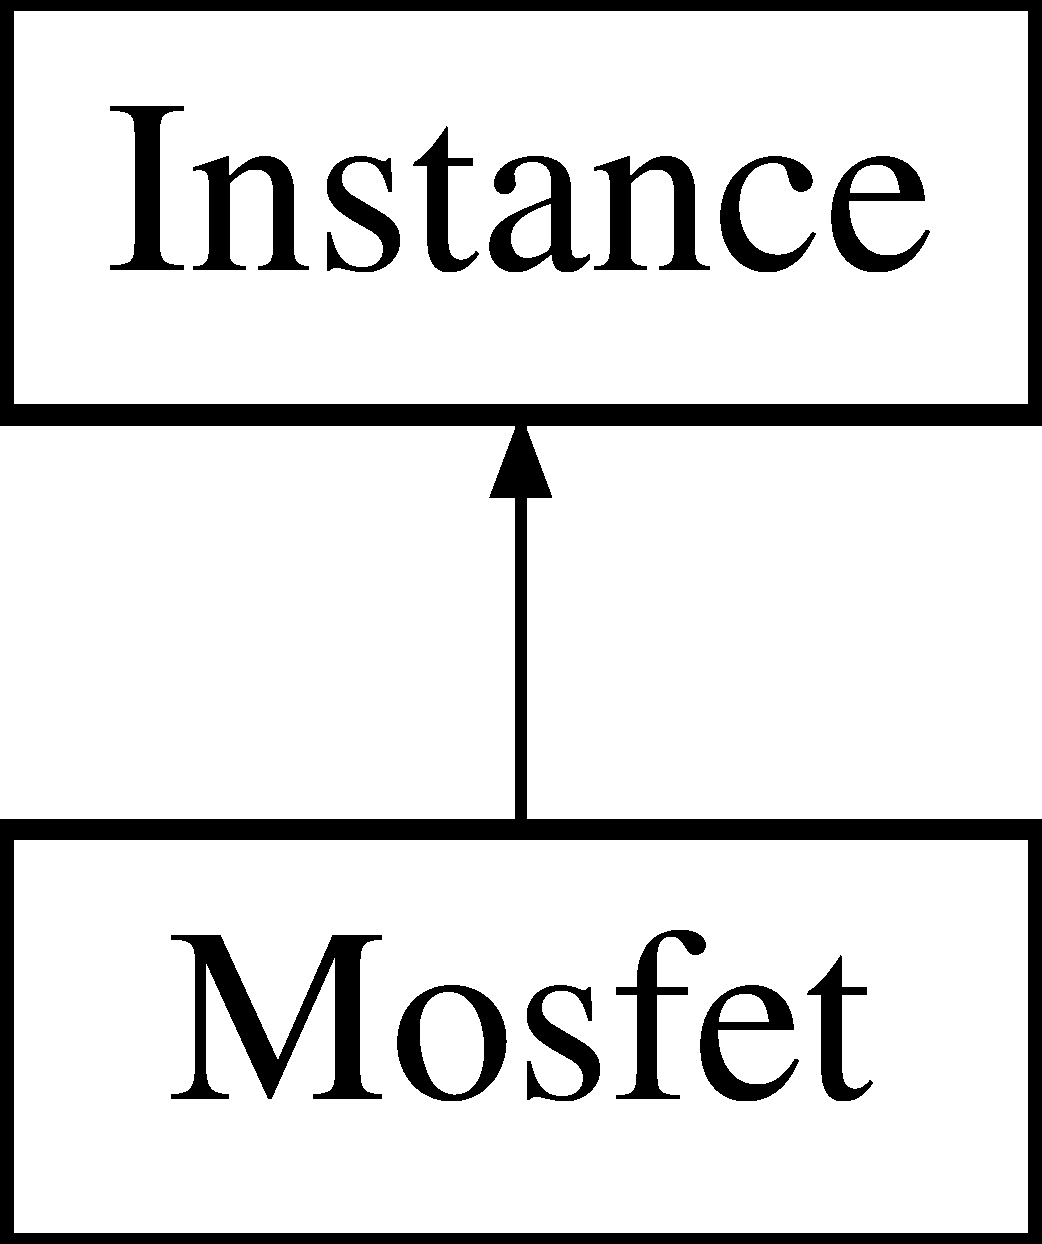
\includegraphics[height=2.000000cm]{class_s_p_i_c_e_1_1_mosfet}
\end{center}
\end{figure}
\subsection*{Public Member Functions}
\begin{DoxyCompactItemize}
\item 
\mbox{\Hypertarget{class_s_p_i_c_e_1_1_mosfet_a56484a169335450d6043ee20086ead93}\label{class_s_p_i_c_e_1_1_mosfet_a56484a169335450d6043ee20086ead93}} 
std\+::string \mbox{\hyperlink{class_s_p_i_c_e_1_1_mosfet_a56484a169335450d6043ee20086ead93}{get\+Bulk}} ()
\begin{DoxyCompactList}\small\item\em returns the bulk connector of the transistor. \end{DoxyCompactList}\item 
\mbox{\Hypertarget{class_s_p_i_c_e_1_1_mosfet_a7265f0565b8368070a3f09c6197a4e9b}\label{class_s_p_i_c_e_1_1_mosfet_a7265f0565b8368070a3f09c6197a4e9b}} 
std\+::string \mbox{\hyperlink{class_s_p_i_c_e_1_1_mosfet_a7265f0565b8368070a3f09c6197a4e9b}{get\+Drain}} ()
\begin{DoxyCompactList}\small\item\em returns the drain connector of the transistor. \end{DoxyCompactList}\item 
\mbox{\Hypertarget{class_s_p_i_c_e_1_1_mosfet_a796d77755aac0828419f55ba2226bf15}\label{class_s_p_i_c_e_1_1_mosfet_a796d77755aac0828419f55ba2226bf15}} 
std\+::string \mbox{\hyperlink{class_s_p_i_c_e_1_1_mosfet_a796d77755aac0828419f55ba2226bf15}{get\+Grid}} ()
\begin{DoxyCompactList}\small\item\em returns the grid connector of the transistor. \end{DoxyCompactList}\item 
\mbox{\Hypertarget{class_s_p_i_c_e_1_1_mosfet_a1791f52b6b5043823c6f3376e8453e3a}\label{class_s_p_i_c_e_1_1_mosfet_a1791f52b6b5043823c6f3376e8453e3a}} 
std\+::string \mbox{\hyperlink{class_s_p_i_c_e_1_1_mosfet_a1791f52b6b5043823c6f3376e8453e3a}{get\+Source}} ()
\begin{DoxyCompactList}\small\item\em returns the source connector of the transistor. \end{DoxyCompactList}\item 
\mbox{\hyperlink{class_s_p_i_c_e_1_1_mosfet_a4f54a31aad6137a6426fb9bfe8947bcf}{Mosfet}} (std\+::string name, std\+::string nd, std\+::string ng, std\+::string ns, std\+::string nb, std\+::string model)
\begin{DoxyCompactList}\small\item\em creates a new mosfet transistor. \end{DoxyCompactList}\end{DoxyCompactItemize}


\subsection{Detailed Description}
This class describes a mosfet transistor which is a specialized instance which has four connectors (grid, drain, source and bulk). 

\subsection{Constructor \& Destructor Documentation}
\mbox{\Hypertarget{class_s_p_i_c_e_1_1_mosfet_a4f54a31aad6137a6426fb9bfe8947bcf}\label{class_s_p_i_c_e_1_1_mosfet_a4f54a31aad6137a6426fb9bfe8947bcf}} 
\index{S\+P\+I\+C\+E\+::\+Mosfet@{S\+P\+I\+C\+E\+::\+Mosfet}!Mosfet@{Mosfet}}
\index{Mosfet@{Mosfet}!S\+P\+I\+C\+E\+::\+Mosfet@{S\+P\+I\+C\+E\+::\+Mosfet}}
\subsubsection{\texorpdfstring{Mosfet()}{Mosfet()}}
{\footnotesize\ttfamily \mbox{\hyperlink{class_s_p_i_c_e_1_1_mosfet}{Mosfet}} (\begin{DoxyParamCaption}\item[{std\+::string}]{name,  }\item[{std\+::string}]{drain,  }\item[{std\+::string}]{grid,  }\item[{std\+::string}]{source,  }\item[{std\+::string}]{bulk,  }\item[{std\+::string}]{model }\end{DoxyParamCaption})\hspace{0.3cm}{\ttfamily [inline]}}



creates a new mosfet transistor. 


\begin{DoxyParams}{Parameters}
{\em name} & the name of the transistor. \\
\hline
{\em drain} & the drain connector of the transistor. \\
\hline
{\em grid} & the grid connector of the transistor. \\
\hline
{\em source} & the source connector of the transistor. \\
\hline
{\em bulk} & the bulk connector of the transistor. \\
\hline
{\em model} & the model of the transistor. \\
\hline
\end{DoxyParams}

\hypertarget{class_name}{}\section{Name Class Reference}
\label{class_name}\index{Name@{Name}}


\subsection{Detailed Description}
This class provides an automatic management of shared name. 
\hypertarget{class_net}{}\section{Net Class Reference}
\label{class_net}\index{Net@{Net}}
\subsection*{Data Structures}
\begin{DoxyCompactItemize}
\item 
class \mbox{\hyperlink{class_net_1_1_connection}{Connection}}
\end{DoxyCompactItemize}


\subsection{Detailed Description}
This class describes a \mbox{\hyperlink{class_net}{Net}}. 
\hypertarget{class_netlist}{}\section{Netlist Class Reference}
\label{class_netlist}\index{Netlist@{Netlist}}


\subsection{Detailed Description}
This class describes a netlist.

A netlist contains the list of all circuit\textquotesingle{}s instances and nets.

\begin{DoxyNote}{Note}
A \mbox{\hyperlink{class_circuit}{Circuit}} must have one and only netlist. If no netlist is defined the \mbox{\hyperlink{class_circuit}{Circuit}} cannot be driven to file. 
\end{DoxyNote}

\hypertarget{class_node}{}\section{Node Class Reference}
\label{class_node}\index{Node@{Node}}


\subsection{Detailed Description}
This class describes a node of the placement tree.

This is an abstract class used to easily managed blocs and groups of the placement tree. 
\hypertarget{class_open_chams_exception}{}\section{Open\+Chams\+Exception Class Reference}
\label{class_open_chams_exception}\index{Open\+Chams\+Exception@{Open\+Chams\+Exception}}


\subsection{Detailed Description}
This class describes the exceptions throwed by the Open\+Chams library in case of errors. 
\hypertarget{class_operator}{}\section{Operator Class Reference}
\label{class_operator}\index{Operator@{Operator}}
\subsection*{Data Structures}
\begin{DoxyCompactItemize}
\item 
class \mbox{\hyperlink{class_operator_1_1_constraint}{Constraint}}
\end{DoxyCompactItemize}


\subsection{Detailed Description}
This class describes an operator of a sizing procedure. 
\hypertarget{class_parameters}{}\section{Parameters Class Reference}
\label{class_parameters}\index{Parameters@{Parameters}}


\subsection{Detailed Description}
This class describes a set of \mbox{\hyperlink{class_parameters}{Parameters}}. \mbox{\hyperlink{class_parameters}{Parameters}} consist in two maps associating a parameter name to a double value or a std\+::string (equation). 
\hypertarget{class_c_i_f_1_1_polygon}{}\section{Polygon Class Reference}
\label{class_c_i_f_1_1_polygon}\index{Polygon@{Polygon}}
\subsection*{Public Member Functions}
\begin{DoxyCompactItemize}
\item 
void \mbox{\hyperlink{class_c_i_f_1_1_polygon_ab3047469780327f18539907e1303ea15}{add\+Point}} (long, long)
\begin{DoxyCompactList}\small\item\em adds a point to the polygon. \end{DoxyCompactList}\item 
\mbox{\hyperlink{class_c_i_f_1_1_polygon_a07683a8a7dea6f09aba6997cc99fff5a}{Polygon}} (long)
\begin{DoxyCompactList}\small\item\em creates a new \mbox{\hyperlink{class_c_i_f_1_1_polygon}{Polygon}}. \end{DoxyCompactList}\end{DoxyCompactItemize}


\subsection{Detailed Description}
This class describes a polygon shape, which consists in a set of points (ie (x,y) pair). 

\subsection{Constructor \& Destructor Documentation}
\mbox{\Hypertarget{class_c_i_f_1_1_polygon_a07683a8a7dea6f09aba6997cc99fff5a}\label{class_c_i_f_1_1_polygon_a07683a8a7dea6f09aba6997cc99fff5a}} 
\index{C\+I\+F\+::\+Polygon@{C\+I\+F\+::\+Polygon}!Polygon@{Polygon}}
\index{Polygon@{Polygon}!C\+I\+F\+::\+Polygon@{C\+I\+F\+::\+Polygon}}
\subsubsection{\texorpdfstring{Polygon()}{Polygon()}}
{\footnotesize\ttfamily \mbox{\hyperlink{class_c_i_f_1_1_polygon}{Polygon}} (\begin{DoxyParamCaption}\item[{long}]{layer }\end{DoxyParamCaption})}



creates a new \mbox{\hyperlink{class_c_i_f_1_1_polygon}{Polygon}}. 


\begin{DoxyParams}{Parameters}
{\em layer} & the layer on which the polygon is created. \\
\hline
\end{DoxyParams}


\subsection{Member Function Documentation}
\mbox{\Hypertarget{class_c_i_f_1_1_polygon_ab3047469780327f18539907e1303ea15}\label{class_c_i_f_1_1_polygon_ab3047469780327f18539907e1303ea15}} 
\index{C\+I\+F\+::\+Polygon@{C\+I\+F\+::\+Polygon}!add\+Point@{add\+Point}}
\index{add\+Point@{add\+Point}!C\+I\+F\+::\+Polygon@{C\+I\+F\+::\+Polygon}}
\subsubsection{\texorpdfstring{add\+Point()}{addPoint()}}
{\footnotesize\ttfamily void add\+Point (\begin{DoxyParamCaption}\item[{long}]{x,  }\item[{long}]{y }\end{DoxyParamCaption})}



adds a point to the polygon. 


\begin{DoxyParams}{Parameters}
{\em x} & the x coordinate of the point. \\
\hline
{\em y} & the y coordinate of the point. \\
\hline
\end{DoxyParams}

\hypertarget{class_port}{}\section{Port Class Reference}
\label{class_port}\index{Port@{Port}}


\subsection{Detailed Description}
This class describes port.

A port is used by schematic to position the input/output ports of the circuit.

\begin{DoxyNote}{Note}
Althought the \mbox{\hyperlink{class_port}{Port}} object is related to \mbox{\hyperlink{class_schematic}{Schematic}}, it is handled by \mbox{\hyperlink{class_net}{Net}} object since a port always belongs to a \mbox{\hyperlink{class_net}{Net}}. 
\end{DoxyNote}

\hypertarget{class_port_point}{}\section{Port\+Point Class Reference}
\label{class_port_point}\index{Port\+Point@{Port\+Point}}


\subsection{Detailed Description}
this class describes a wire point associated to a \mbox{\hyperlink{class_port}{Port}}. 
\hypertarget{class_a_g_d_s_1_1_rectangle}{}\section{Rectangle Class Reference}
\label{class_a_g_d_s_1_1_rectangle}\index{Rectangle@{Rectangle}}
Inheritance diagram for Rectangle\+:\begin{figure}[H]
\begin{center}
\leavevmode
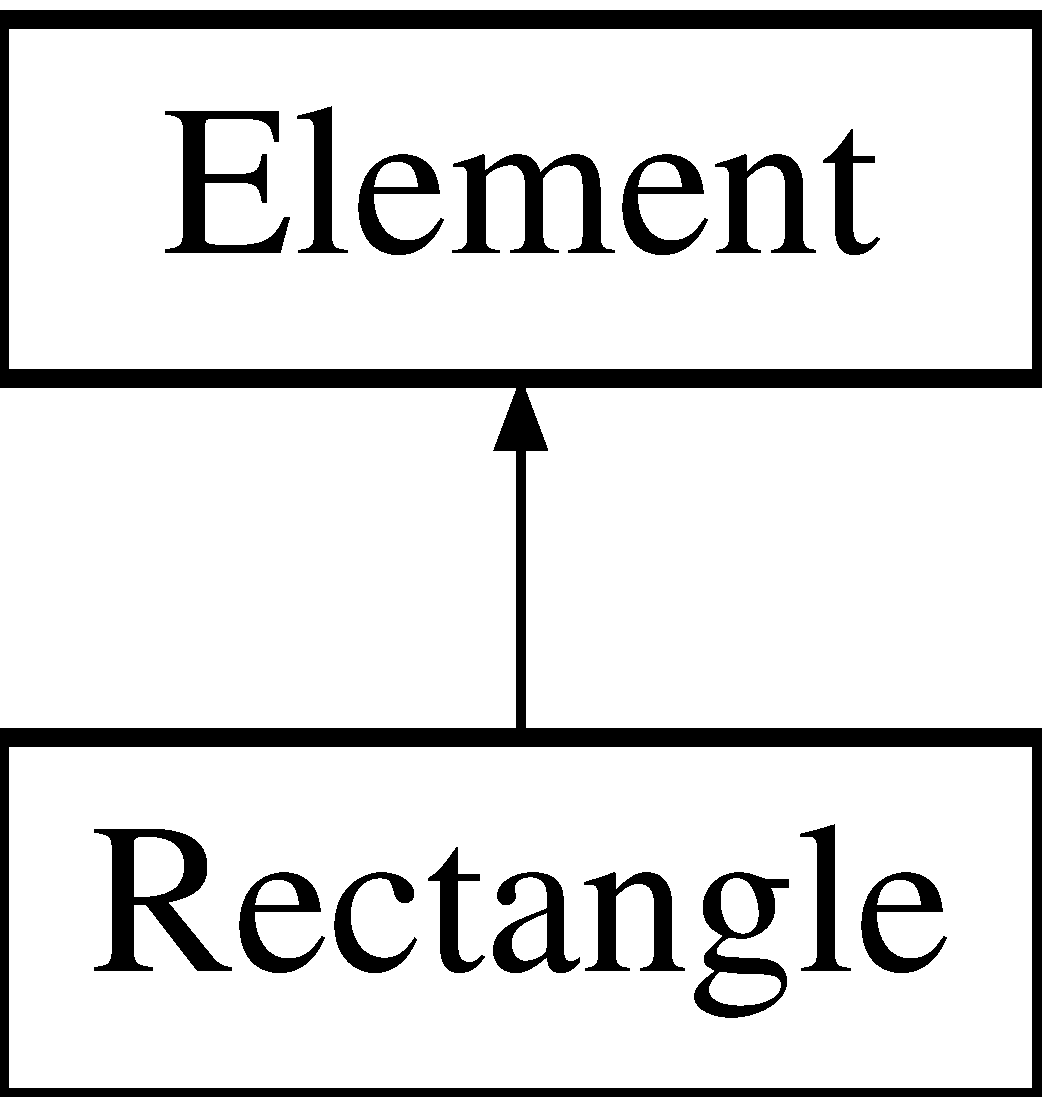
\includegraphics[height=2.000000cm]{class_a_g_d_s_1_1_rectangle}
\end{center}
\end{figure}
\subsection*{Public Member Functions}
\begin{DoxyCompactItemize}
\item 
\mbox{\hyperlink{class_a_g_d_s_1_1_rectangle_a84899edb51e65c78535f0b06b266f11b}{Rectangle}} (int layer, double xmin, double ymin, double xmax, double ymax)
\begin{DoxyCompactList}\small\item\em creates a new \mbox{\hyperlink{class_a_g_d_s_1_1_rectangle}{Rectangle}} \end{DoxyCompactList}\end{DoxyCompactItemize}


\subsection{Detailed Description}
This class describes a rectangle element and inherits from \mbox{\hyperlink{class_a_g_d_s_1_1_element}{A\+G\+D\+S\+::\+Element}}. 

\subsection{Constructor \& Destructor Documentation}
\mbox{\Hypertarget{class_a_g_d_s_1_1_rectangle_a84899edb51e65c78535f0b06b266f11b}\label{class_a_g_d_s_1_1_rectangle_a84899edb51e65c78535f0b06b266f11b}} 
\index{A\+G\+D\+S\+::\+Rectangle@{A\+G\+D\+S\+::\+Rectangle}!Rectangle@{Rectangle}}
\index{Rectangle@{Rectangle}!A\+G\+D\+S\+::\+Rectangle@{A\+G\+D\+S\+::\+Rectangle}}
\subsubsection{\texorpdfstring{Rectangle()}{Rectangle()}}
{\footnotesize\ttfamily \mbox{\hyperlink{class_a_g_d_s_1_1_rectangle}{Rectangle}} (\begin{DoxyParamCaption}\item[{int}]{layer,  }\item[{double}]{xmin,  }\item[{double}]{ymin,  }\item[{double}]{xmax,  }\item[{double}]{ymax }\end{DoxyParamCaption})}



creates a new \mbox{\hyperlink{class_a_g_d_s_1_1_rectangle}{Rectangle}} 


\begin{DoxyParams}{Parameters}
{\em layer} & the layer number into which the rectangle shape is drawned. \\
\hline
{\em xmin} & the x coordinate of the bottom-\/left corner of the rectangle. \\
\hline
{\em ymin} & the y coordinate of the bottom-\/left corner of the rectangle. \\
\hline
{\em xmax} & the x coordinate of the top-\/right corner of the rectangle. \\
\hline
{\em ymax} & the y coordinate of the top-\/right corner of the rectangle. \\
\hline
\end{DoxyParams}

\hypertarget{class_s_p_i_c_e_1_1_resistor}{}\section{Resistor Class Reference}
\label{class_s_p_i_c_e_1_1_resistor}\index{Resistor@{Resistor}}
Inheritance diagram for Resistor\+:\begin{figure}[H]
\begin{center}
\leavevmode
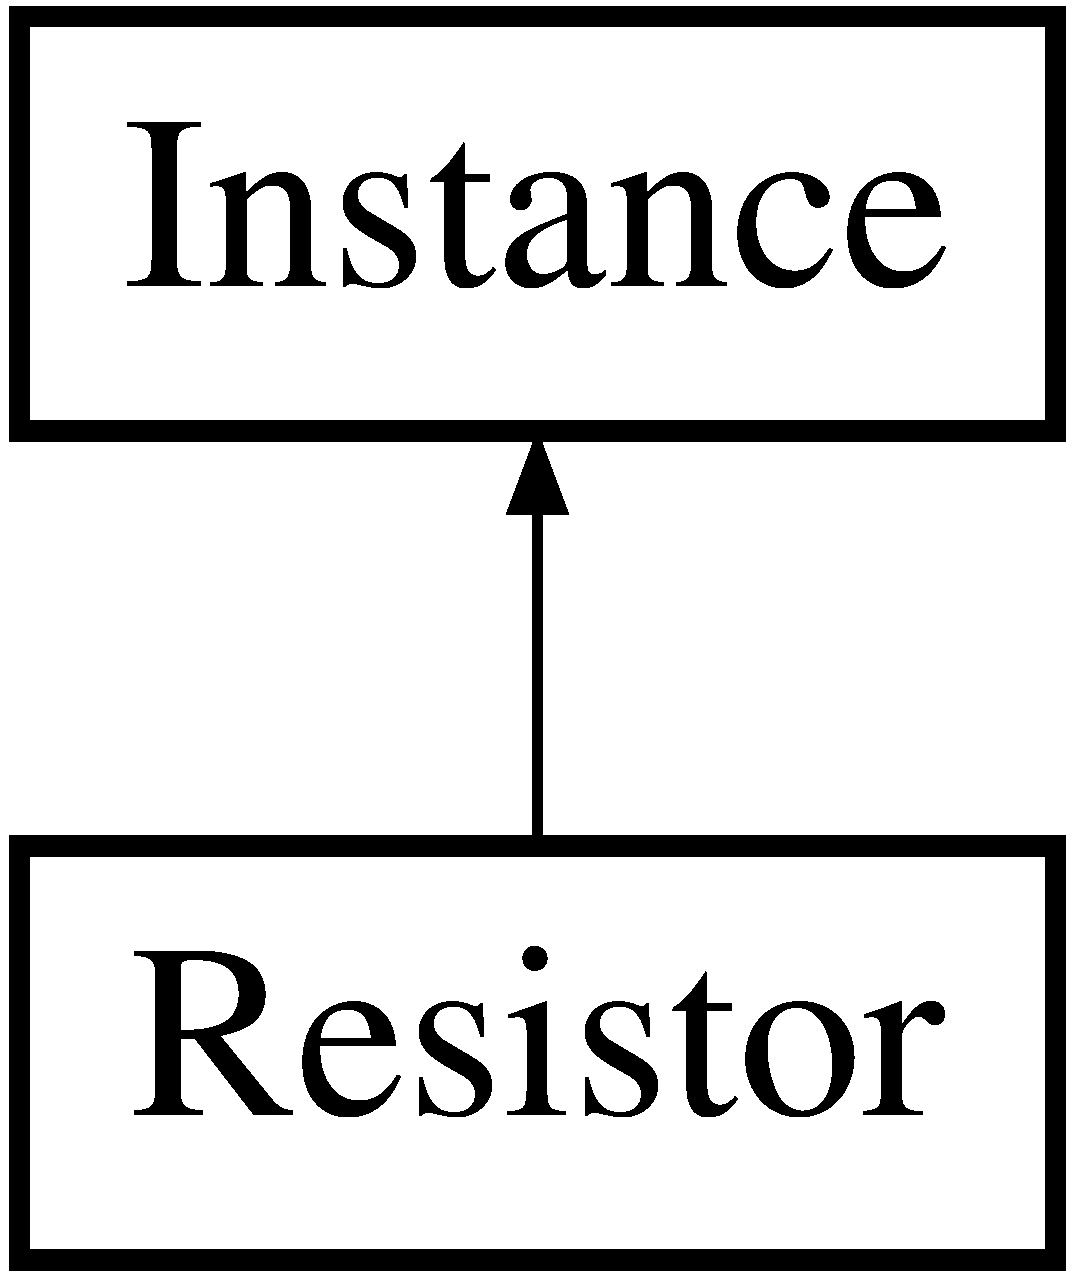
\includegraphics[height=2.000000cm]{class_s_p_i_c_e_1_1_resistor}
\end{center}
\end{figure}
\subsection*{Public Member Functions}
\begin{DoxyCompactItemize}
\item 
\mbox{\Hypertarget{class_s_p_i_c_e_1_1_resistor_ab57aa52f48a5a56c89dd49eae66c1a0f}\label{class_s_p_i_c_e_1_1_resistor_ab57aa52f48a5a56c89dd49eae66c1a0f}} 
std\+::string \mbox{\hyperlink{class_s_p_i_c_e_1_1_resistor_ab57aa52f48a5a56c89dd49eae66c1a0f}{get\+First}} ()
\begin{DoxyCompactList}\small\item\em returns the first connector of the resistor. \end{DoxyCompactList}\item 
\mbox{\Hypertarget{class_s_p_i_c_e_1_1_resistor_a9665313821b2fca41e14b9865133af7f}\label{class_s_p_i_c_e_1_1_resistor_a9665313821b2fca41e14b9865133af7f}} 
std\+::string \mbox{\hyperlink{class_s_p_i_c_e_1_1_resistor_a9665313821b2fca41e14b9865133af7f}{get\+Second}} ()
\begin{DoxyCompactList}\small\item\em returns the second connector of the resistor. \end{DoxyCompactList}\item 
\mbox{\Hypertarget{class_s_p_i_c_e_1_1_resistor_a4c052cb2622c580a250b2c783a436882}\label{class_s_p_i_c_e_1_1_resistor_a4c052cb2622c580a250b2c783a436882}} 
std\+::string \mbox{\hyperlink{class_s_p_i_c_e_1_1_resistor_a4c052cb2622c580a250b2c783a436882}{get\+Value}} ()
\begin{DoxyCompactList}\small\item\em returns the value of the resistor. \end{DoxyCompactList}\item 
\mbox{\hyperlink{class_s_p_i_c_e_1_1_resistor_aa4e89fab1189113134e98edbb0c622bf}{Resistor}} (std\+::string name, std\+::string first, std\+::string second, std\+::string value)
\begin{DoxyCompactList}\small\item\em creates a new resistor. \end{DoxyCompactList}\end{DoxyCompactItemize}


\subsection{Detailed Description}
This class describes a resistor which is a specialized instance which has two connectors and a value. 

\subsection{Constructor \& Destructor Documentation}
\mbox{\Hypertarget{class_s_p_i_c_e_1_1_resistor_aa4e89fab1189113134e98edbb0c622bf}\label{class_s_p_i_c_e_1_1_resistor_aa4e89fab1189113134e98edbb0c622bf}} 
\index{S\+P\+I\+C\+E\+::\+Resistor@{S\+P\+I\+C\+E\+::\+Resistor}!Resistor@{Resistor}}
\index{Resistor@{Resistor}!S\+P\+I\+C\+E\+::\+Resistor@{S\+P\+I\+C\+E\+::\+Resistor}}
\subsubsection{\texorpdfstring{Resistor()}{Resistor()}}
{\footnotesize\ttfamily \mbox{\hyperlink{class_s_p_i_c_e_1_1_resistor}{Resistor}} (\begin{DoxyParamCaption}\item[{std\+::string}]{name,  }\item[{std\+::string}]{first,  }\item[{std\+::string}]{second,  }\item[{std\+::string}]{value }\end{DoxyParamCaption})\hspace{0.3cm}{\ttfamily [inline]}}



creates a new resistor. 


\begin{DoxyParams}{Parameters}
{\em name} & the name of the resistor. \\
\hline
{\em first} & the first connector of the resistor. \\
\hline
{\em second} & the second connector of the resistor. \\
\hline
{\em value} & the value of the resistor. \\
\hline
\end{DoxyParams}

\hypertarget{class_d_t_r_1_1_rule}{}\section{Rule Class Reference}
\label{class_d_t_r_1_1_rule}\index{Rule@{Rule}}
Inheritance diagram for Rule\+:\begin{figure}[H]
\begin{center}
\leavevmode
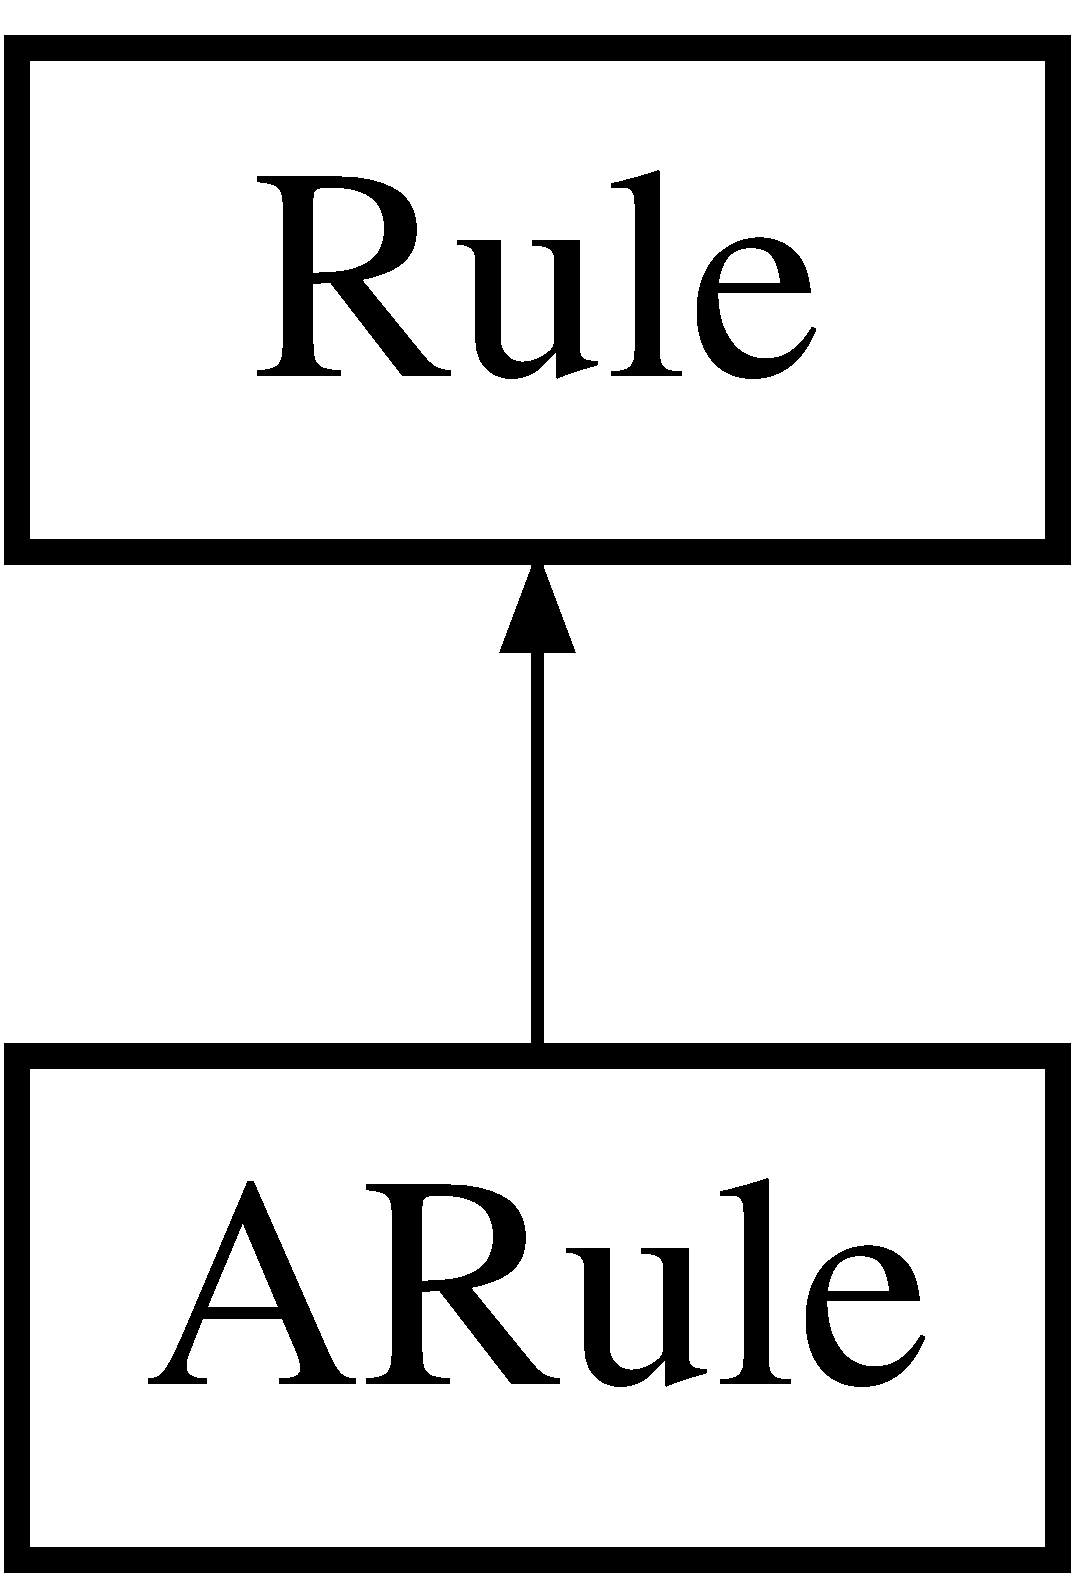
\includegraphics[height=2.000000cm]{class_d_t_r_1_1_rule}
\end{center}
\end{figure}
\subsection*{Public Member Functions}
\begin{DoxyCompactItemize}
\item 
\mbox{\Hypertarget{class_d_t_r_1_1_rule_a710e6d75d7ae8de075ced5da150e10db}\label{class_d_t_r_1_1_rule_a710e6d75d7ae8de075ced5da150e10db}} 
const std\+::string \& \mbox{\hyperlink{class_d_t_r_1_1_rule_a710e6d75d7ae8de075ced5da150e10db}{get\+Layer1}} ()
\begin{DoxyCompactList}\small\item\em returns the first layer of the rule. \end{DoxyCompactList}\item 
\mbox{\Hypertarget{class_d_t_r_1_1_rule_a29e6dc8d83450a582cbd9af372e96162}\label{class_d_t_r_1_1_rule_a29e6dc8d83450a582cbd9af372e96162}} 
virtual const std\+::string \& \mbox{\hyperlink{class_d_t_r_1_1_rule_a29e6dc8d83450a582cbd9af372e96162}{get\+Layer2}} ()
\begin{DoxyCompactList}\small\item\em returns the second layer of the rule. \end{DoxyCompactList}\item 
\mbox{\Hypertarget{class_d_t_r_1_1_rule_a2858c0c4e8b5108f041237cf5a802029}\label{class_d_t_r_1_1_rule_a2858c0c4e8b5108f041237cf5a802029}} 
const std\+::string \& \mbox{\hyperlink{class_d_t_r_1_1_rule_a2858c0c4e8b5108f041237cf5a802029}{get\+Name}} ()
\begin{DoxyCompactList}\small\item\em returns the name of the rule. \end{DoxyCompactList}\item 
\mbox{\Hypertarget{class_d_t_r_1_1_rule_a07cf74adaf661f0aaaa1818d24c2243d}\label{class_d_t_r_1_1_rule_a07cf74adaf661f0aaaa1818d24c2243d}} 
const std\+::string \& \mbox{\hyperlink{class_d_t_r_1_1_rule_a07cf74adaf661f0aaaa1818d24c2243d}{get\+Ref}} ()
\begin{DoxyCompactList}\small\item\em returns the reference of the rule. \end{DoxyCompactList}\item 
const std\+::string \& \mbox{\hyperlink{class_d_t_r_1_1_rule_a7a88ff26f0ba9cfbfa5059c565d1e30b}{get\+Type}} ()
\begin{DoxyCompactList}\small\item\em returns the type of the rule. \end{DoxyCompactList}\item 
\mbox{\Hypertarget{class_d_t_r_1_1_rule_a666f992950731c68de1ad441f80f228c}\label{class_d_t_r_1_1_rule_a666f992950731c68de1ad441f80f228c}} 
double \mbox{\hyperlink{class_d_t_r_1_1_rule_a666f992950731c68de1ad441f80f228c}{get\+Value}} ()
\begin{DoxyCompactList}\small\item\em returns the value of the rule. \end{DoxyCompactList}\item 
\mbox{\Hypertarget{class_d_t_r_1_1_rule_a3fad3e4886891e1efcdca530d2f6daa3}\label{class_d_t_r_1_1_rule_a3fad3e4886891e1efcdca530d2f6daa3}} 
const std\+::string \& \mbox{\hyperlink{class_d_t_r_1_1_rule_a3fad3e4886891e1efcdca530d2f6daa3}{get\+Value\+As\+String}} ()
\begin{DoxyCompactList}\small\item\em returns the string corresponding to the value of the rule. \end{DoxyCompactList}\item 
\mbox{\hyperlink{class_d_t_r_1_1_rule_aee8c5385eba121203f788a012b502e24}{Rule}} (const char $\ast$name, double value, const char $\ast$ref, const char $\ast$layer1, const char $\ast$layer2)
\begin{DoxyCompactList}\small\item\em creates a new rule. \end{DoxyCompactList}\item 
void \mbox{\hyperlink{class_d_t_r_1_1_rule_a3568407d7a7890c39b8c9acc1e608535}{set\+Type}} (const char $\ast$)
\begin{DoxyCompactList}\small\item\em sets the type of a rule. \end{DoxyCompactList}\end{DoxyCompactItemize}


\subsection{Detailed Description}
This class describes a symmetrical rule.

A symmetrical rule represents several type of rules\+:
\begin{DoxyItemize}
\item a simple rule with only a name (e.\+g. transistor\+MinW\+: transistor minimum width)
\item a rule for a unique layer (e.\+g. min\+Width.\+metal1\+: the minimum width for metal1 wire)
\item a rule associating two layers (e.\+g min\+Space.\+poly.\+active\+: the minimum spacing between a poly shape and an active shape) In this last case the symmetrical characteristic is important since it implies that the value is the same if we invert the two layers \+: min\+Spacing poly vs active = min\+Spacing active vs poly.
\end{DoxyItemize}

Typical rules using no layer are\+: {\itshape transistor\+MinW, transsitor\+MaxW, transistor\+MinL transistor\+MaxL}

Typical rules using one layer are\+: {\itshape min\+Width, min\+Spacing, min\+Area, min\+Gate\+Spacing, min\+Strap\+Enclosure}

Typical rules using two layers are\+: {\itshape min\+Spacing} 

\subsection{Constructor \& Destructor Documentation}
\mbox{\Hypertarget{class_d_t_r_1_1_rule_aee8c5385eba121203f788a012b502e24}\label{class_d_t_r_1_1_rule_aee8c5385eba121203f788a012b502e24}} 
\index{D\+T\+R\+::\+Rule@{D\+T\+R\+::\+Rule}!Rule@{Rule}}
\index{Rule@{Rule}!D\+T\+R\+::\+Rule@{D\+T\+R\+::\+Rule}}
\subsubsection{\texorpdfstring{Rule()}{Rule()}}
{\footnotesize\ttfamily \mbox{\hyperlink{class_d_t_r_1_1_rule}{Rule}} (\begin{DoxyParamCaption}\item[{const char $\ast$}]{name,  }\item[{double}]{value,  }\item[{const char $\ast$}]{ref,  }\item[{const char $\ast$}]{layer1,  }\item[{const char $\ast$}]{layer2 }\end{DoxyParamCaption})\hspace{0.3cm}{\ttfamily [inline]}}



creates a new rule. 


\begin{DoxyParams}{Parameters}
{\em name} & the name of the rule. \\
\hline
{\em value} & the value of the rule. \\
\hline
{\em ref} & the reference of the rule (helpful to find rule in design kit). \\
\hline
{\em layer1} & the first layer. \\
\hline
{\em layer2} & the second layer. \\
\hline
\end{DoxyParams}


\subsection{Member Function Documentation}
\mbox{\Hypertarget{class_d_t_r_1_1_rule_a7a88ff26f0ba9cfbfa5059c565d1e30b}\label{class_d_t_r_1_1_rule_a7a88ff26f0ba9cfbfa5059c565d1e30b}} 
\index{D\+T\+R\+::\+Rule@{D\+T\+R\+::\+Rule}!get\+Type@{get\+Type}}
\index{get\+Type@{get\+Type}!D\+T\+R\+::\+Rule@{D\+T\+R\+::\+Rule}}
\subsubsection{\texorpdfstring{get\+Type()}{getType()}}
{\footnotesize\ttfamily const std\+::string \& get\+Type (\begin{DoxyParamCaption}{ }\end{DoxyParamCaption})\hspace{0.3cm}{\ttfamily [inline]}}



returns the type of the rule. 

\mbox{\hyperlink{class_d_t_r_1_1_rule}{Rule}}\textquotesingle{}s type allows to set a specific type for a rule especially the \textquotesingle{}area\textquotesingle{} type to take into account that the value of the rule is to be considered in unit$^\wedge$2. \mbox{\Hypertarget{class_d_t_r_1_1_rule_a3568407d7a7890c39b8c9acc1e608535}\label{class_d_t_r_1_1_rule_a3568407d7a7890c39b8c9acc1e608535}} 
\index{D\+T\+R\+::\+Rule@{D\+T\+R\+::\+Rule}!set\+Type@{set\+Type}}
\index{set\+Type@{set\+Type}!D\+T\+R\+::\+Rule@{D\+T\+R\+::\+Rule}}
\subsubsection{\texorpdfstring{set\+Type()}{setType()}}
{\footnotesize\ttfamily void set\+Type (\begin{DoxyParamCaption}\item[{const char $\ast$}]{type }\end{DoxyParamCaption})\hspace{0.3cm}{\ttfamily [inline]}}



sets the type of a rule. 


\begin{DoxyParams}{Parameters}
{\em type} & the type of the rule.\\
\hline
\end{DoxyParams}
\begin{DoxyNote}{Note}
By default the type of a rule is \char`\"{}\char`\"{}. 
\end{DoxyNote}

\hypertarget{class_schematic}{}\section{Schematic Class Reference}
\label{class_schematic}\index{Schematic@{Schematic}}
\subsection*{Data Structures}
\begin{DoxyCompactItemize}
\item 
class \mbox{\hyperlink{class_schematic_1_1_infos}{Infos}}
\end{DoxyCompactItemize}


\subsection{Detailed Description}
This class describes schematic informations.

The \mbox{\hyperlink{class_schematic}{Schematic}} object is used to store all informations relative to schematic of the circuit.

\begin{DoxyNote}{Note}
The \mbox{\hyperlink{class_schematic}{Schematic}} object is optionnal in \mbox{\hyperlink{class_circuit}{Circuit}}. 
\end{DoxyNote}

\hypertarget{class_simul_model}{}\section{Simul\+Model Class Reference}
\label{class_simul_model}\index{Simul\+Model@{Simul\+Model}}


\subsection{Detailed Description}
This class describes a simulation model used by \mbox{\hyperlink{class_operator}{Operator}} in \mbox{\hyperlink{class_sizing}{Sizing}} procedure. 
\hypertarget{class_sizing}{}\section{Sizing Class Reference}
\label{class_sizing}\index{Sizing@{Sizing}}


\subsection{Detailed Description}
This class describes a sizing procedure.

The \mbox{\hyperlink{class_sizing}{Sizing}} object is used to store all informations relative to sizing procedure as we defined it in {\bfseries C\+H\+A\+MS}.

\begin{DoxyNote}{Note}
The \mbox{\hyperlink{class_sizing}{Sizing}} object is optionnal in \mbox{\hyperlink{class_circuit}{Circuit}}. 
\end{DoxyNote}

\hypertarget{class_s_p_i_c_e_1_1_source}{}\section{Source Class Reference}
\label{class_s_p_i_c_e_1_1_source}\index{Source@{Source}}
Inheritance diagram for Source\+:\begin{figure}[H]
\begin{center}
\leavevmode
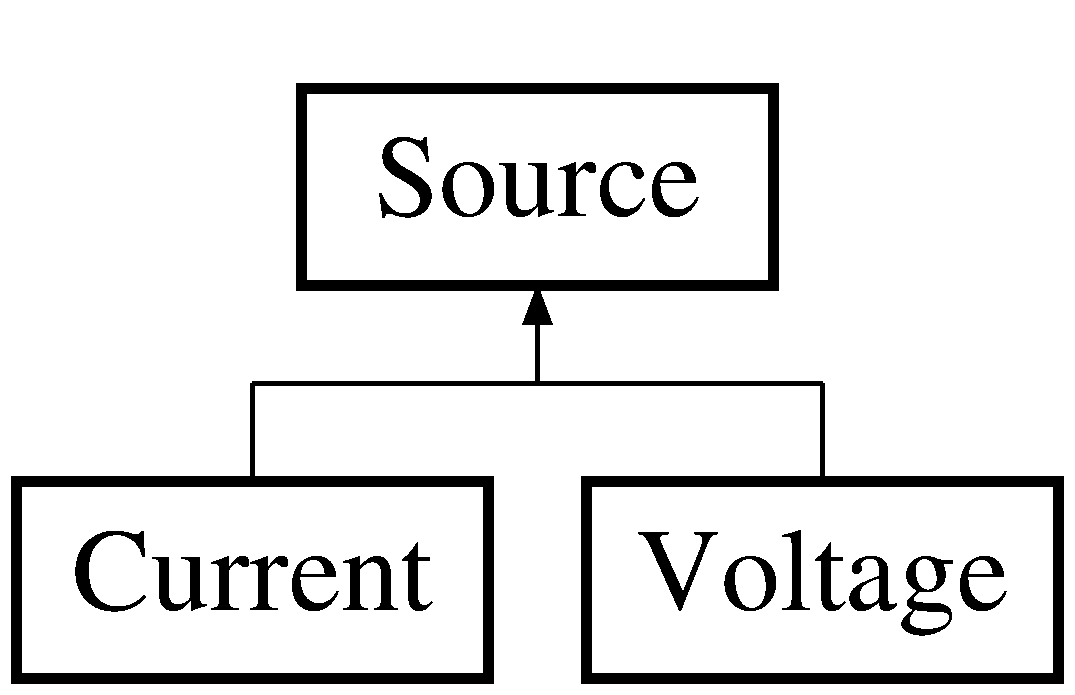
\includegraphics[height=2.000000cm]{class_s_p_i_c_e_1_1_source}
\end{center}
\end{figure}
\subsection*{Public Member Functions}
\begin{DoxyCompactItemize}
\item 
\mbox{\Hypertarget{class_s_p_i_c_e_1_1_source_ac0fc966d4386ddb71d99361e3fccb311}\label{class_s_p_i_c_e_1_1_source_ac0fc966d4386ddb71d99361e3fccb311}} 
std\+::string \mbox{\hyperlink{class_s_p_i_c_e_1_1_source_ac0fc966d4386ddb71d99361e3fccb311}{get\+Name}} ()
\begin{DoxyCompactList}\small\item\em returns the name of the source. \end{DoxyCompactList}\item 
\mbox{\Hypertarget{class_s_p_i_c_e_1_1_source_a8b4ab73ed1d99c533aa22af0a37ebb0d}\label{class_s_p_i_c_e_1_1_source_a8b4ab73ed1d99c533aa22af0a37ebb0d}} 
std\+::string \mbox{\hyperlink{class_s_p_i_c_e_1_1_source_a8b4ab73ed1d99c533aa22af0a37ebb0d}{get\+Negative}} ()
\begin{DoxyCompactList}\small\item\em returns the negative connector of the source. \end{DoxyCompactList}\item 
\mbox{\Hypertarget{class_s_p_i_c_e_1_1_source_a1adb347b9a2c2da556e4417ab0eec0e1}\label{class_s_p_i_c_e_1_1_source_a1adb347b9a2c2da556e4417ab0eec0e1}} 
std\+::string \mbox{\hyperlink{class_s_p_i_c_e_1_1_source_a1adb347b9a2c2da556e4417ab0eec0e1}{get\+Positive}} ()
\begin{DoxyCompactList}\small\item\em returns the positive connector of the source. \end{DoxyCompactList}\item 
\mbox{\Hypertarget{class_s_p_i_c_e_1_1_source_a4c052cb2622c580a250b2c783a436882}\label{class_s_p_i_c_e_1_1_source_a4c052cb2622c580a250b2c783a436882}} 
std\+::string \mbox{\hyperlink{class_s_p_i_c_e_1_1_source_a4c052cb2622c580a250b2c783a436882}{get\+Value}} ()
\begin{DoxyCompactList}\small\item\em returns the value of the source. \end{DoxyCompactList}\end{DoxyCompactItemize}
\subsection*{Protected Member Functions}
\begin{DoxyCompactItemize}
\item 
\mbox{\hyperlink{class_s_p_i_c_e_1_1_source_a35145400f091a09eed7baa19128a3bc8}{Source}} (std\+::string name, std\+::string pos, std\+::string neg, std\+::string value)
\begin{DoxyCompactList}\small\item\em creates a new source. \end{DoxyCompactList}\end{DoxyCompactItemize}


\subsection{Detailed Description}
This abstract class is a base class for \mbox{\hyperlink{class_s_p_i_c_e_1_1_current}{S\+P\+I\+C\+E\+::\+Current}} and \mbox{\hyperlink{class_s_p_i_c_e_1_1_voltage}{S\+P\+I\+C\+E\+::\+Voltage}} sources. 

\subsection{Constructor \& Destructor Documentation}
\mbox{\Hypertarget{class_s_p_i_c_e_1_1_source_a35145400f091a09eed7baa19128a3bc8}\label{class_s_p_i_c_e_1_1_source_a35145400f091a09eed7baa19128a3bc8}} 
\index{S\+P\+I\+C\+E\+::\+Source@{S\+P\+I\+C\+E\+::\+Source}!Source@{Source}}
\index{Source@{Source}!S\+P\+I\+C\+E\+::\+Source@{S\+P\+I\+C\+E\+::\+Source}}
\subsubsection{\texorpdfstring{Source()}{Source()}}
{\footnotesize\ttfamily \mbox{\hyperlink{class_s_p_i_c_e_1_1_source}{Source}} (\begin{DoxyParamCaption}\item[{std\+::string}]{name,  }\item[{std\+::string}]{pos,  }\item[{std\+::string}]{neg,  }\item[{std\+::string}]{value }\end{DoxyParamCaption})\hspace{0.3cm}{\ttfamily [inline]}, {\ttfamily [protected]}}



creates a new source. 


\begin{DoxyParams}{Parameters}
{\em name} & the name of the source. \\
\hline
{\em pos} & the positive connector of the source. \\
\hline
{\em neg} & the negative connector of the source. \\
\hline
{\em value} & the value of the source. \\
\hline
\end{DoxyParams}

\hypertarget{class_s_p_i_c_e_1_1_spice_exception}{}\section{Spice\+Exception Class Reference}
\label{class_s_p_i_c_e_1_1_spice_exception}\index{Spice\+Exception@{Spice\+Exception}}


\subsection{Detailed Description}
This class describes the exceptions throwed by the Spice library in case of errors. 
\hypertarget{class_a_g_d_s_1_1_structure}{}\section{Structure Class Reference}
\label{class_a_g_d_s_1_1_structure}\index{Structure@{Structure}}
\subsection*{Public Member Functions}
\begin{DoxyCompactItemize}
\item 
bool \mbox{\hyperlink{class_a_g_d_s_1_1_structure_a2dd203e6770f7d15d6f706867c919a60}{add\+Element}} (\mbox{\hyperlink{class_a_g_d_s_1_1_element}{Element}} $\ast$)
\begin{DoxyCompactList}\small\item\em adds an \mbox{\hyperlink{class_a_g_d_s_1_1_element}{Element}} to the \mbox{\hyperlink{class_a_g_d_s_1_1_structure}{Structure}}. \end{DoxyCompactList}\item 
\mbox{\Hypertarget{class_a_g_d_s_1_1_structure_ac0fc966d4386ddb71d99361e3fccb311}\label{class_a_g_d_s_1_1_structure_ac0fc966d4386ddb71d99361e3fccb311}} 
std\+::string \mbox{\hyperlink{class_a_g_d_s_1_1_structure_ac0fc966d4386ddb71d99361e3fccb311}{get\+Name}} ()
\begin{DoxyCompactList}\small\item\em returns the name of the \mbox{\hyperlink{class_a_g_d_s_1_1_structure}{Structure}}. \end{DoxyCompactList}\item 
\mbox{\hyperlink{class_a_g_d_s_1_1_structure_a797bfd2e6684bb9870c8070b4ef6ff41}{Structure}} (std\+::string str\+Name)
\begin{DoxyCompactList}\small\item\em creates a new \mbox{\hyperlink{class_a_g_d_s_1_1_structure}{Structure}} \end{DoxyCompactList}\end{DoxyCompactItemize}


\subsection{Detailed Description}
This class describes a G\+DS \mbox{\hyperlink{class_a_g_d_s_1_1_structure}{Structure}} with a name and a list of Elements. 

\subsection{Constructor \& Destructor Documentation}
\mbox{\Hypertarget{class_a_g_d_s_1_1_structure_a797bfd2e6684bb9870c8070b4ef6ff41}\label{class_a_g_d_s_1_1_structure_a797bfd2e6684bb9870c8070b4ef6ff41}} 
\index{A\+G\+D\+S\+::\+Structure@{A\+G\+D\+S\+::\+Structure}!Structure@{Structure}}
\index{Structure@{Structure}!A\+G\+D\+S\+::\+Structure@{A\+G\+D\+S\+::\+Structure}}
\subsubsection{\texorpdfstring{Structure()}{Structure()}}
{\footnotesize\ttfamily \mbox{\hyperlink{class_a_g_d_s_1_1_structure}{Structure}} (\begin{DoxyParamCaption}\item[{std\+::string}]{name }\end{DoxyParamCaption})}



creates a new \mbox{\hyperlink{class_a_g_d_s_1_1_structure}{Structure}} 


\begin{DoxyParams}{Parameters}
{\em name} & the name of the structure. \\
\hline
\end{DoxyParams}


\subsection{Member Function Documentation}
\mbox{\Hypertarget{class_a_g_d_s_1_1_structure_a2dd203e6770f7d15d6f706867c919a60}\label{class_a_g_d_s_1_1_structure_a2dd203e6770f7d15d6f706867c919a60}} 
\index{A\+G\+D\+S\+::\+Structure@{A\+G\+D\+S\+::\+Structure}!add\+Element@{add\+Element}}
\index{add\+Element@{add\+Element}!A\+G\+D\+S\+::\+Structure@{A\+G\+D\+S\+::\+Structure}}
\subsubsection{\texorpdfstring{add\+Element()}{addElement()}}
{\footnotesize\ttfamily bool add\+Element (\begin{DoxyParamCaption}\item[{\mbox{\hyperlink{class_a_g_d_s_1_1_element}{Element}} $\ast$}]{element }\end{DoxyParamCaption})}



adds an \mbox{\hyperlink{class_a_g_d_s_1_1_element}{Element}} to the \mbox{\hyperlink{class_a_g_d_s_1_1_structure}{Structure}}. 


\begin{DoxyParams}{Parameters}
{\em element} & the \mbox{\hyperlink{class_a_g_d_s_1_1_element}{Element}} object to add. \\
\hline
\end{DoxyParams}

\hypertarget{class_s_p_i_c_e_1_1_subckt}{}\section{Subckt Class Reference}
\label{class_s_p_i_c_e_1_1_subckt}\index{Subckt@{Subckt}}
\subsection*{Public Member Functions}
\begin{DoxyCompactItemize}
\item 
void \mbox{\hyperlink{class_s_p_i_c_e_1_1_subckt_a6c590c1d92248d6e5f95ea6c470fbb5a}{add\+Comment}} (std\+::string)
\begin{DoxyCompactList}\small\item\em adds a comment to the subckt. \end{DoxyCompactList}\item 
void \mbox{\hyperlink{class_s_p_i_c_e_1_1_subckt_a7bb4a4532643568ab1ac2c229185a88e}{add\+Instance}} (\mbox{\hyperlink{class_s_p_i_c_e_1_1_instance}{Instance}} $\ast$)
\begin{DoxyCompactList}\small\item\em adds an instance to the subckt. \end{DoxyCompactList}\item 
void \mbox{\hyperlink{class_s_p_i_c_e_1_1_subckt_ac162264683fa3d9b3384d3e8cc291fa2}{add\+Interface}} (std\+::string)
\begin{DoxyCompactList}\small\item\em adds an interface to the subckt. \end{DoxyCompactList}\item 
void \mbox{\hyperlink{class_s_p_i_c_e_1_1_subckt_ab3ab147a16bc490ce96db905a4ca271c}{add\+Parameter}} (std\+::string, std\+::string)
\begin{DoxyCompactList}\small\item\em adds a parameter to the subckt. \end{DoxyCompactList}\item 
const std\+::vector$<$ std\+::string $>$ \& \mbox{\hyperlink{class_s_p_i_c_e_1_1_subckt_aa4a73ef909ceb8d442ed2f205967613a}{get\+Comments}} ()
\begin{DoxyCompactList}\small\item\em returns the comments of the subckt. \end{DoxyCompactList}\item 
\mbox{\Hypertarget{class_s_p_i_c_e_1_1_subckt_a8e6e58ffab876152a740092520c35d73}\label{class_s_p_i_c_e_1_1_subckt_a8e6e58ffab876152a740092520c35d73}} 
const std\+::vector$<$ \mbox{\hyperlink{class_s_p_i_c_e_1_1_instance}{Instance}} $\ast$ $>$ \& \mbox{\hyperlink{class_s_p_i_c_e_1_1_subckt_a8e6e58ffab876152a740092520c35d73}{get\+Instances}} ()
\begin{DoxyCompactList}\small\item\em returns the instances of the subckt. \end{DoxyCompactList}\item 
\mbox{\Hypertarget{class_s_p_i_c_e_1_1_subckt_a5df00fe6eb5e287abef28c76ce88bd1e}\label{class_s_p_i_c_e_1_1_subckt_a5df00fe6eb5e287abef28c76ce88bd1e}} 
const std\+::vector$<$ std\+::string $>$ \& \mbox{\hyperlink{class_s_p_i_c_e_1_1_subckt_a5df00fe6eb5e287abef28c76ce88bd1e}{get\+Interfaces}} ()
\begin{DoxyCompactList}\small\item\em returns the interfaces of the subckt. \end{DoxyCompactList}\item 
\mbox{\Hypertarget{class_s_p_i_c_e_1_1_subckt_af55b1fe10eacd22c7ff3544b5ed32ef3}\label{class_s_p_i_c_e_1_1_subckt_af55b1fe10eacd22c7ff3544b5ed32ef3}} 
const std\+::string \mbox{\hyperlink{class_s_p_i_c_e_1_1_subckt_af55b1fe10eacd22c7ff3544b5ed32ef3}{get\+Name}} ()
\begin{DoxyCompactList}\small\item\em returns the name of the subckt. \end{DoxyCompactList}\item 
\mbox{\Hypertarget{class_s_p_i_c_e_1_1_subckt_aee7d59083b78d31ac5c19ab508da91e0}\label{class_s_p_i_c_e_1_1_subckt_aee7d59083b78d31ac5c19ab508da91e0}} 
const std\+::map$<$ std\+::string, std\+::string $>$ \& \mbox{\hyperlink{class_s_p_i_c_e_1_1_subckt_aee7d59083b78d31ac5c19ab508da91e0}{get\+Parameters}} ()
\begin{DoxyCompactList}\small\item\em returns the parameters of the subckt. \end{DoxyCompactList}\item 
\mbox{\hyperlink{class_s_p_i_c_e_1_1_subckt_a5b9ee31a0302af435029f29a93b29d7d}{Subckt}} (std\+::string name)
\begin{DoxyCompactList}\small\item\em creates a new subckt. \end{DoxyCompactList}\end{DoxyCompactItemize}


\subsection{Detailed Description}
This class describes a subckt of the global circuit. 

\subsection{Constructor \& Destructor Documentation}
\mbox{\Hypertarget{class_s_p_i_c_e_1_1_subckt_a5b9ee31a0302af435029f29a93b29d7d}\label{class_s_p_i_c_e_1_1_subckt_a5b9ee31a0302af435029f29a93b29d7d}} 
\index{S\+P\+I\+C\+E\+::\+Subckt@{S\+P\+I\+C\+E\+::\+Subckt}!Subckt@{Subckt}}
\index{Subckt@{Subckt}!S\+P\+I\+C\+E\+::\+Subckt@{S\+P\+I\+C\+E\+::\+Subckt}}
\subsubsection{\texorpdfstring{Subckt()}{Subckt()}}
{\footnotesize\ttfamily \mbox{\hyperlink{class_s_p_i_c_e_1_1_subckt}{Subckt}} (\begin{DoxyParamCaption}\item[{std\+::string}]{name }\end{DoxyParamCaption})\hspace{0.3cm}{\ttfamily [inline]}}



creates a new subckt. 


\begin{DoxyParams}{Parameters}
{\em name} & the name of the subckt \\
\hline
\end{DoxyParams}


\subsection{Member Function Documentation}
\mbox{\Hypertarget{class_s_p_i_c_e_1_1_subckt_a6c590c1d92248d6e5f95ea6c470fbb5a}\label{class_s_p_i_c_e_1_1_subckt_a6c590c1d92248d6e5f95ea6c470fbb5a}} 
\index{S\+P\+I\+C\+E\+::\+Subckt@{S\+P\+I\+C\+E\+::\+Subckt}!add\+Comment@{add\+Comment}}
\index{add\+Comment@{add\+Comment}!S\+P\+I\+C\+E\+::\+Subckt@{S\+P\+I\+C\+E\+::\+Subckt}}
\subsubsection{\texorpdfstring{add\+Comment()}{addComment()}}
{\footnotesize\ttfamily void add\+Comment (\begin{DoxyParamCaption}\item[{std\+::string}]{comment }\end{DoxyParamCaption})\hspace{0.3cm}{\ttfamily [inline]}}



adds a comment to the subckt. 


\begin{DoxyParams}{Parameters}
{\em comment} & the comment to add.\\
\hline
\end{DoxyParams}
\begin{DoxyNote}{Note}
comments of a subckt are the first lines of the subckt to describe the interfaces of the subckt. 
\end{DoxyNote}
\mbox{\Hypertarget{class_s_p_i_c_e_1_1_subckt_a7bb4a4532643568ab1ac2c229185a88e}\label{class_s_p_i_c_e_1_1_subckt_a7bb4a4532643568ab1ac2c229185a88e}} 
\index{S\+P\+I\+C\+E\+::\+Subckt@{S\+P\+I\+C\+E\+::\+Subckt}!add\+Instance@{add\+Instance}}
\index{add\+Instance@{add\+Instance}!S\+P\+I\+C\+E\+::\+Subckt@{S\+P\+I\+C\+E\+::\+Subckt}}
\subsubsection{\texorpdfstring{add\+Instance()}{addInstance()}}
{\footnotesize\ttfamily void add\+Instance (\begin{DoxyParamCaption}\item[{\mbox{\hyperlink{class_s_p_i_c_e_1_1_instance}{Instance}} $\ast$}]{instance }\end{DoxyParamCaption})\hspace{0.3cm}{\ttfamily [inline]}}



adds an instance to the subckt. 


\begin{DoxyParams}{Parameters}
{\em instance} & the instance to add. \\
\hline
\end{DoxyParams}
\mbox{\Hypertarget{class_s_p_i_c_e_1_1_subckt_ac162264683fa3d9b3384d3e8cc291fa2}\label{class_s_p_i_c_e_1_1_subckt_ac162264683fa3d9b3384d3e8cc291fa2}} 
\index{S\+P\+I\+C\+E\+::\+Subckt@{S\+P\+I\+C\+E\+::\+Subckt}!add\+Interface@{add\+Interface}}
\index{add\+Interface@{add\+Interface}!S\+P\+I\+C\+E\+::\+Subckt@{S\+P\+I\+C\+E\+::\+Subckt}}
\subsubsection{\texorpdfstring{add\+Interface()}{addInterface()}}
{\footnotesize\ttfamily void add\+Interface (\begin{DoxyParamCaption}\item[{std\+::string}]{name }\end{DoxyParamCaption})\hspace{0.3cm}{\ttfamily [inline]}}



adds an interface to the subckt. 


\begin{DoxyParams}{Parameters}
{\em name} & the name of the interface to add. \\
\hline
\end{DoxyParams}
\mbox{\Hypertarget{class_s_p_i_c_e_1_1_subckt_ab3ab147a16bc490ce96db905a4ca271c}\label{class_s_p_i_c_e_1_1_subckt_ab3ab147a16bc490ce96db905a4ca271c}} 
\index{S\+P\+I\+C\+E\+::\+Subckt@{S\+P\+I\+C\+E\+::\+Subckt}!add\+Parameter@{add\+Parameter}}
\index{add\+Parameter@{add\+Parameter}!S\+P\+I\+C\+E\+::\+Subckt@{S\+P\+I\+C\+E\+::\+Subckt}}
\subsubsection{\texorpdfstring{add\+Parameter()}{addParameter()}}
{\footnotesize\ttfamily void add\+Parameter (\begin{DoxyParamCaption}\item[{std\+::string}]{name,  }\item[{std\+::string}]{value }\end{DoxyParamCaption})}



adds a parameter to the subckt. 


\begin{DoxyParams}{Parameters}
{\em name} & the name of the parameter to add. \\
\hline
{\em value} & the value of the parameter to add. \\
\hline
\end{DoxyParams}
\mbox{\Hypertarget{class_s_p_i_c_e_1_1_subckt_aa4a73ef909ceb8d442ed2f205967613a}\label{class_s_p_i_c_e_1_1_subckt_aa4a73ef909ceb8d442ed2f205967613a}} 
\index{S\+P\+I\+C\+E\+::\+Subckt@{S\+P\+I\+C\+E\+::\+Subckt}!get\+Comments@{get\+Comments}}
\index{get\+Comments@{get\+Comments}!S\+P\+I\+C\+E\+::\+Subckt@{S\+P\+I\+C\+E\+::\+Subckt}}
\subsubsection{\texorpdfstring{get\+Comments()}{getComments()}}
{\footnotesize\ttfamily const std\+::vector$<$ std\+::string $>$ \& get\+Comments (\begin{DoxyParamCaption}{ }\end{DoxyParamCaption})\hspace{0.3cm}{\ttfamily [inline]}}



returns the comments of the subckt. 

\begin{DoxyNote}{Note}
comments of a subckt are the first lines of the subckt to describe the interfaces of the subckt. 
\end{DoxyNote}

\hypertarget{class_d_t_r_1_1_techno}{}\section{Techno Class Reference}
\label{class_d_t_r_1_1_techno}\index{Techno@{Techno}}
\subsection*{Public Member Functions}
\begin{DoxyCompactItemize}
\item 
\mbox{\hyperlink{class_d_t_r_1_1_a_rule}{A\+Rule}} $\ast$ \mbox{\hyperlink{class_d_t_r_1_1_techno_a5f5a790974fe7d3b1c6f1b698ef0a818}{add\+A\+Rule}} (const char $\ast$name, double value, const char $\ast$ref, const char $\ast$layer1, const char $\ast$layer2)
\begin{DoxyCompactList}\small\item\em creates a new \mbox{\hyperlink{class_d_t_r_1_1_a_rule}{A\+Rule}} and adds it to the \mbox{\hyperlink{class_d_t_r_1_1_techno}{Techno}} object. \end{DoxyCompactList}\item 
\mbox{\hyperlink{class_d_t_r_1_1_rule}{Rule}} $\ast$ \mbox{\hyperlink{class_d_t_r_1_1_techno_afa2c8412c365c950649b9f81661ecafd}{add\+Rule}} (const char $\ast$name, double value, const char $\ast$ref, const char $\ast$layer1=\char`\"{}\char`\"{}, const char $\ast$layer2=\char`\"{}\char`\"{})
\begin{DoxyCompactList}\small\item\em creates a new \mbox{\hyperlink{class_d_t_r_1_1_rule}{Rule}} and adds it the to \mbox{\hyperlink{class_d_t_r_1_1_techno}{Techno}} object. \end{DoxyCompactList}\item 
\mbox{\Hypertarget{class_d_t_r_1_1_techno_a3fd7335faa33dce2f87c7e50eef3e294}\label{class_d_t_r_1_1_techno_a3fd7335faa33dce2f87c7e50eef3e294}} 
const std\+::string \& \mbox{\hyperlink{class_d_t_r_1_1_techno_a3fd7335faa33dce2f87c7e50eef3e294}{get\+Name}} () const
\begin{DoxyCompactList}\small\item\em returns the name of the technology. \end{DoxyCompactList}\item 
\mbox{\hyperlink{class_d_t_r_1_1_rule}{Rule}} $\ast$ \mbox{\hyperlink{class_d_t_r_1_1_techno_a4d56a05b47bd6c51e4e18120f49b584b}{get\+Rule}} (const char $\ast$name, const char $\ast$layer1=\char`\"{}\char`\"{}, const char $\ast$layer2=\char`\"{}\char`\"{})
\begin{DoxyCompactList}\small\item\em returns the rule uniquely identified by its name and layers. \end{DoxyCompactList}\item 
std\+::vector$<$ \mbox{\hyperlink{class_d_t_r_1_1_rule}{Rule}} $\ast$ $>$ \& \mbox{\hyperlink{class_d_t_r_1_1_techno_ac322d0479195cd8a65ff5a922b7f2af7}{get\+Rules}} ()
\begin{DoxyCompactList}\small\item\em returns a reference on the std\+::vector containing all technology\textquotesingle{}s rules. \end{DoxyCompactList}\item 
\mbox{\Hypertarget{class_d_t_r_1_1_techno_a42e12e8f890c03ebf12e754d7e489dcb}\label{class_d_t_r_1_1_techno_a42e12e8f890c03ebf12e754d7e489dcb}} 
const std\+::string \& \mbox{\hyperlink{class_d_t_r_1_1_techno_a42e12e8f890c03ebf12e754d7e489dcb}{get\+Unit}} () const
\begin{DoxyCompactList}\small\item\em returns the unit. \end{DoxyCompactList}\item 
double \mbox{\hyperlink{class_d_t_r_1_1_techno_ac08e2e60dd16750551221ca908001057}{get\+Value}} (const char $\ast$name, const char $\ast$layer1=\char`\"{}\char`\"{}, const char $\ast$layer2=\char`\"{}\char`\"{})
\begin{DoxyCompactList}\small\item\em returns the value of a rule uniquely identified by its name and layers. \end{DoxyCompactList}\item 
const std\+::string \& \mbox{\hyperlink{class_d_t_r_1_1_techno_ad5ef5b8e444ab7a86a2e3bff7762c956}{get\+Value\+As\+String}} (const char $\ast$name, const char $\ast$layer1=\char`\"{}\char`\"{}, const char $\ast$layer2=\char`\"{}\char`\"{})
\begin{DoxyCompactList}\small\item\em returns a string corresponding to the value of a rule uniquely identified by its name and layers. \end{DoxyCompactList}\item 
\mbox{\hyperlink{class_d_t_r_1_1_techno_a25c6aecdd011d09618908626192c933f}{Techno}} (const char $\ast$name, const char $\ast$unit, const char $\ast$version)
\begin{DoxyCompactList}\small\item\em creates a new technology \end{DoxyCompactList}\item 
bool \mbox{\hyperlink{class_d_t_r_1_1_techno_a26b05539dd3345963b8708788b82e2cb}{write\+To\+File}} (const char $\ast$file\+Path)
\begin{DoxyCompactList}\small\item\em writes the database to file. \end{DoxyCompactList}\end{DoxyCompactItemize}
\subsection*{Static Public Member Functions}
\begin{DoxyCompactItemize}
\item 
static \mbox{\hyperlink{class_d_t_r_1_1_techno}{Techno}} $\ast$ \mbox{\hyperlink{class_d_t_r_1_1_techno_acf863c2bdb7f1aacc4422c8155c60d17}{read\+From\+File}} (const char $\ast$file\+Path)
\begin{DoxyCompactList}\small\item\em creates and returns a \mbox{\hyperlink{class_d_t_r_1_1_techno}{Techno}} object based on a database source file. \end{DoxyCompactList}\end{DoxyCompactItemize}


\subsection{Detailed Description}
This class contains generic informations such as the name of the technology and the unit used, and the list of all technologic rules. 

\subsection{Constructor \& Destructor Documentation}
\mbox{\Hypertarget{class_d_t_r_1_1_techno_a25c6aecdd011d09618908626192c933f}\label{class_d_t_r_1_1_techno_a25c6aecdd011d09618908626192c933f}} 
\index{D\+T\+R\+::\+Techno@{D\+T\+R\+::\+Techno}!Techno@{Techno}}
\index{Techno@{Techno}!D\+T\+R\+::\+Techno@{D\+T\+R\+::\+Techno}}
\subsubsection{\texorpdfstring{Techno()}{Techno()}}
{\footnotesize\ttfamily \mbox{\hyperlink{class_d_t_r_1_1_techno}{Techno}} (\begin{DoxyParamCaption}\item[{const char $\ast$}]{name,  }\item[{const char $\ast$}]{unit,  }\item[{const char $\ast$}]{version }\end{DoxyParamCaption})}



creates a new technology 


\begin{DoxyParams}{Parameters}
{\em name} & the name of the technology. \\
\hline
{\em unit} & the unit used for all values. \\
\hline
{\em version} & the technology version/revision. \\
\hline
\end{DoxyParams}


\subsection{Member Function Documentation}
\mbox{\Hypertarget{class_d_t_r_1_1_techno_a5f5a790974fe7d3b1c6f1b698ef0a818}\label{class_d_t_r_1_1_techno_a5f5a790974fe7d3b1c6f1b698ef0a818}} 
\index{D\+T\+R\+::\+Techno@{D\+T\+R\+::\+Techno}!add\+A\+Rule@{add\+A\+Rule}}
\index{add\+A\+Rule@{add\+A\+Rule}!D\+T\+R\+::\+Techno@{D\+T\+R\+::\+Techno}}
\subsubsection{\texorpdfstring{add\+A\+Rule()}{addARule()}}
{\footnotesize\ttfamily \mbox{\hyperlink{class_d_t_r_1_1_a_rule}{A\+Rule}} $\ast$ add\+A\+Rule (\begin{DoxyParamCaption}\item[{const char $\ast$}]{name,  }\item[{double}]{value,  }\item[{const char $\ast$}]{ref,  }\item[{const char $\ast$}]{layer1,  }\item[{const char $\ast$}]{layer2 }\end{DoxyParamCaption})}



creates a new \mbox{\hyperlink{class_d_t_r_1_1_a_rule}{A\+Rule}} and adds it to the \mbox{\hyperlink{class_d_t_r_1_1_techno}{Techno}} object. 


\begin{DoxyParams}{Parameters}
{\em name} & the name of the rule. \\
\hline
{\em value} & the value of the rule. \\
\hline
{\em ref} & the reference of the rule (helpful to find the rule in design kit). \\
\hline
{\em layer1} & the first layer. \\
\hline
{\em layer2} & the second layer.\\
\hline
\end{DoxyParams}
\begin{DoxyReturn}{Returns}
the newly created \mbox{\hyperlink{class_d_t_r_1_1_a_rule}{A\+Rule}} object. 
\end{DoxyReturn}
\mbox{\Hypertarget{class_d_t_r_1_1_techno_afa2c8412c365c950649b9f81661ecafd}\label{class_d_t_r_1_1_techno_afa2c8412c365c950649b9f81661ecafd}} 
\index{D\+T\+R\+::\+Techno@{D\+T\+R\+::\+Techno}!add\+Rule@{add\+Rule}}
\index{add\+Rule@{add\+Rule}!D\+T\+R\+::\+Techno@{D\+T\+R\+::\+Techno}}
\subsubsection{\texorpdfstring{add\+Rule()}{addRule()}}
{\footnotesize\ttfamily \mbox{\hyperlink{class_d_t_r_1_1_rule}{Rule}} $\ast$ add\+Rule (\begin{DoxyParamCaption}\item[{const char $\ast$}]{name,  }\item[{double}]{value,  }\item[{const char $\ast$}]{ref,  }\item[{const char $\ast$}]{layer1 = {\ttfamily \char`\"{}\char`\"{}},  }\item[{const char $\ast$}]{layer2 = {\ttfamily \char`\"{}\char`\"{}} }\end{DoxyParamCaption})}



creates a new \mbox{\hyperlink{class_d_t_r_1_1_rule}{Rule}} and adds it the to \mbox{\hyperlink{class_d_t_r_1_1_techno}{Techno}} object. 


\begin{DoxyParams}{Parameters}
{\em name} & the name of the rule. \\
\hline
{\em value} & the value of the rule. \\
\hline
{\em ref} & the reference of the rule (helpful to find the rule in design kit). \\
\hline
{\em layer1} & the first layer. This is an optionnal argument, default value is \char`\"{}\char`\"{}. \\
\hline
{\em layer2} & the second layer. This is an optionnal argument, default value is \char`\"{}\char`\"{}.\\
\hline
\end{DoxyParams}
\begin{DoxyReturn}{Returns}
the newly created \mbox{\hyperlink{class_d_t_r_1_1_rule}{Rule}} object. 
\end{DoxyReturn}
\mbox{\Hypertarget{class_d_t_r_1_1_techno_a4d56a05b47bd6c51e4e18120f49b584b}\label{class_d_t_r_1_1_techno_a4d56a05b47bd6c51e4e18120f49b584b}} 
\index{D\+T\+R\+::\+Techno@{D\+T\+R\+::\+Techno}!get\+Rule@{get\+Rule}}
\index{get\+Rule@{get\+Rule}!D\+T\+R\+::\+Techno@{D\+T\+R\+::\+Techno}}
\subsubsection{\texorpdfstring{get\+Rule()}{getRule()}}
{\footnotesize\ttfamily \mbox{\hyperlink{class_d_t_r_1_1_rule}{Rule}} $\ast$ get\+Rule (\begin{DoxyParamCaption}\item[{const char $\ast$}]{name,  }\item[{const char $\ast$}]{layer1 = {\ttfamily \char`\"{}\char`\"{}},  }\item[{const char $\ast$}]{layer2 = {\ttfamily \char`\"{}\char`\"{}} }\end{DoxyParamCaption})}



returns the rule uniquely identified by its name and layers. 


\begin{DoxyParams}{Parameters}
{\em name} & the name of the rule. \\
\hline
{\em layer1} & the first layer. This is an optionnal argument, default value is \char`\"{}\char`\"{}. \\
\hline
{\em layer2} & the second layer. This is an optionnal argument, default value is \char`\"{}\char`\"{}.\\
\hline
\end{DoxyParams}
\begin{DoxyReturn}{Returns}
the rule. 
\end{DoxyReturn}
\mbox{\Hypertarget{class_d_t_r_1_1_techno_ac322d0479195cd8a65ff5a922b7f2af7}\label{class_d_t_r_1_1_techno_ac322d0479195cd8a65ff5a922b7f2af7}} 
\index{D\+T\+R\+::\+Techno@{D\+T\+R\+::\+Techno}!get\+Rules@{get\+Rules}}
\index{get\+Rules@{get\+Rules}!D\+T\+R\+::\+Techno@{D\+T\+R\+::\+Techno}}
\subsubsection{\texorpdfstring{get\+Rules()}{getRules()}}
{\footnotesize\ttfamily std\+::vector$<$ \mbox{\hyperlink{class_d_t_r_1_1_rule}{Rule}} $\ast$ $>$ \& get\+Rules (\begin{DoxyParamCaption}{ }\end{DoxyParamCaption})\hspace{0.3cm}{\ttfamily [inline]}}



returns a reference on the std\+::vector containing all technology\textquotesingle{}s rules. 

\begin{DoxyNote}{Note}
this method is not yet available in python 
\end{DoxyNote}
\mbox{\Hypertarget{class_d_t_r_1_1_techno_ac08e2e60dd16750551221ca908001057}\label{class_d_t_r_1_1_techno_ac08e2e60dd16750551221ca908001057}} 
\index{D\+T\+R\+::\+Techno@{D\+T\+R\+::\+Techno}!get\+Value@{get\+Value}}
\index{get\+Value@{get\+Value}!D\+T\+R\+::\+Techno@{D\+T\+R\+::\+Techno}}
\subsubsection{\texorpdfstring{get\+Value()}{getValue()}}
{\footnotesize\ttfamily double get\+Value (\begin{DoxyParamCaption}\item[{const char $\ast$}]{name,  }\item[{const char $\ast$}]{layer1 = {\ttfamily \char`\"{}\char`\"{}},  }\item[{const char $\ast$}]{layer2 = {\ttfamily \char`\"{}\char`\"{}} }\end{DoxyParamCaption})}



returns the value of a rule uniquely identified by its name and layers. 


\begin{DoxyParams}{Parameters}
{\em name} & the name of the rule. \\
\hline
{\em layer1} & the first layer. This is an optionnal argument, default value is \char`\"{}\char`\"{}. \\
\hline
{\em layer2} & the second layer. This is an optionnal argument, default value is \char`\"{}\char`\"{}.\\
\hline
\end{DoxyParams}
\begin{DoxyReturn}{Returns}
the value of the rule. 
\end{DoxyReturn}
\mbox{\Hypertarget{class_d_t_r_1_1_techno_ad5ef5b8e444ab7a86a2e3bff7762c956}\label{class_d_t_r_1_1_techno_ad5ef5b8e444ab7a86a2e3bff7762c956}} 
\index{D\+T\+R\+::\+Techno@{D\+T\+R\+::\+Techno}!get\+Value\+As\+String@{get\+Value\+As\+String}}
\index{get\+Value\+As\+String@{get\+Value\+As\+String}!D\+T\+R\+::\+Techno@{D\+T\+R\+::\+Techno}}
\subsubsection{\texorpdfstring{get\+Value\+As\+String()}{getValueAsString()}}
{\footnotesize\ttfamily const string \& get\+Value\+As\+String (\begin{DoxyParamCaption}\item[{const char $\ast$}]{name,  }\item[{const char $\ast$}]{layer1 = {\ttfamily \char`\"{}\char`\"{}},  }\item[{const char $\ast$}]{layer2 = {\ttfamily \char`\"{}\char`\"{}} }\end{DoxyParamCaption})}



returns a string corresponding to the value of a rule uniquely identified by its name and layers. 


\begin{DoxyParams}{Parameters}
{\em name} & the name of the rule. \\
\hline
{\em layer1} & the first layer. This is an optionnal argument, default value is \char`\"{}\char`\"{}. \\
\hline
{\em layer2} & the second layer. This is an optionnal argument, default value is \char`\"{}\char`\"{}.\\
\hline
\end{DoxyParams}
\begin{DoxyReturn}{Returns}
the string corresponding to the value of the rule.
\end{DoxyReturn}
\begin{DoxyNote}{Note}
this method is important for python module since to avoid rounding problems it is necessary to use Decimal object which is build based on a string. 
\end{DoxyNote}
\mbox{\Hypertarget{class_d_t_r_1_1_techno_acf863c2bdb7f1aacc4422c8155c60d17}\label{class_d_t_r_1_1_techno_acf863c2bdb7f1aacc4422c8155c60d17}} 
\index{D\+T\+R\+::\+Techno@{D\+T\+R\+::\+Techno}!read\+From\+File@{read\+From\+File}}
\index{read\+From\+File@{read\+From\+File}!D\+T\+R\+::\+Techno@{D\+T\+R\+::\+Techno}}
\subsubsection{\texorpdfstring{read\+From\+File()}{readFromFile()}}
{\footnotesize\ttfamily \mbox{\hyperlink{class_d_t_r_1_1_techno}{Techno}} $\ast$ read\+From\+File (\begin{DoxyParamCaption}\item[{const char $\ast$}]{filename }\end{DoxyParamCaption})\hspace{0.3cm}{\ttfamily [static]}}



creates and returns a \mbox{\hyperlink{class_d_t_r_1_1_techno}{Techno}} object based on a database source file. 


\begin{DoxyParams}{Parameters}
{\em filename} & the source file name.\\
\hline
\end{DoxyParams}
\begin{DoxyReturn}{Returns}
the newly created \mbox{\hyperlink{class_d_t_r_1_1_techno}{Techno}}. 
\end{DoxyReturn}
\mbox{\Hypertarget{class_d_t_r_1_1_techno_a26b05539dd3345963b8708788b82e2cb}\label{class_d_t_r_1_1_techno_a26b05539dd3345963b8708788b82e2cb}} 
\index{D\+T\+R\+::\+Techno@{D\+T\+R\+::\+Techno}!write\+To\+File@{write\+To\+File}}
\index{write\+To\+File@{write\+To\+File}!D\+T\+R\+::\+Techno@{D\+T\+R\+::\+Techno}}
\subsubsection{\texorpdfstring{write\+To\+File()}{writeToFile()}}
{\footnotesize\ttfamily bool write\+To\+File (\begin{DoxyParamCaption}\item[{const char $\ast$}]{filename }\end{DoxyParamCaption})}



writes the database to file. 


\begin{DoxyParams}{Parameters}
{\em filename} & the destination file name. \\
\hline
\end{DoxyParams}

\hypertarget{class_transistor}{}\section{Transistor Class Reference}
\label{class_transistor}\index{Transistor@{Transistor}}


\subsection{Detailed Description}
This class describes a \mbox{\hyperlink{class_transistor}{Transistor}}.

The transistor object is used to describe the inside of a \mbox{\hyperlink{class_device}{Device}}. The goal is to explicit the connection between the transistor and the device\textquotesingle{}s nets. 
\hypertarget{class_s_p_i_c_e_1_1_value}{}\section{Value Class Reference}
\label{class_s_p_i_c_e_1_1_value}\index{Value@{Value}}

\hypertarget{class_s_p_i_c_e_1_1_voltage}{}\section{Voltage Class Reference}
\label{class_s_p_i_c_e_1_1_voltage}\index{Voltage@{Voltage}}
Inheritance diagram for Voltage\+:\begin{figure}[H]
\begin{center}
\leavevmode
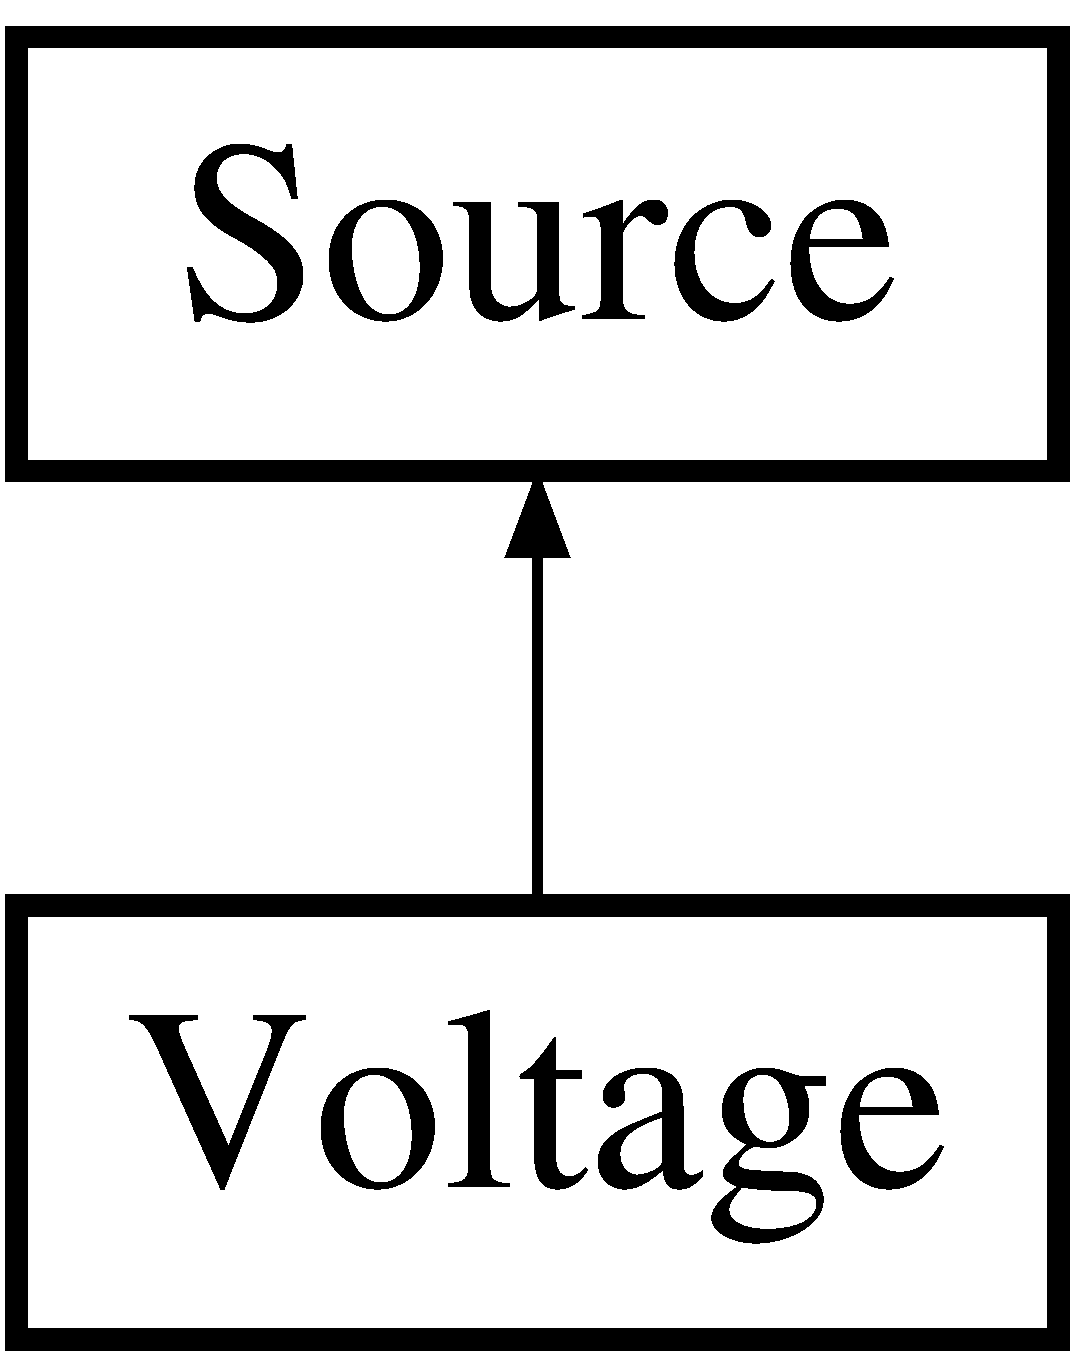
\includegraphics[height=2.000000cm]{class_s_p_i_c_e_1_1_voltage}
\end{center}
\end{figure}
\subsection*{Public Member Functions}
\begin{DoxyCompactItemize}
\item 
\mbox{\hyperlink{class_s_p_i_c_e_1_1_voltage_ae88c0ca0c1c79404c71ed3f4851a933d}{Voltage}} (std\+::string name, std\+::string pos, std\+::string neg, std\+::string value)
\begin{DoxyCompactList}\small\item\em creates a new voltage source. \end{DoxyCompactList}\end{DoxyCompactItemize}
\subsection*{Additional Inherited Members}


\subsection{Detailed Description}
This class describes a voltage source. 

\subsection{Constructor \& Destructor Documentation}
\mbox{\Hypertarget{class_s_p_i_c_e_1_1_voltage_ae88c0ca0c1c79404c71ed3f4851a933d}\label{class_s_p_i_c_e_1_1_voltage_ae88c0ca0c1c79404c71ed3f4851a933d}} 
\index{S\+P\+I\+C\+E\+::\+Voltage@{S\+P\+I\+C\+E\+::\+Voltage}!Voltage@{Voltage}}
\index{Voltage@{Voltage}!S\+P\+I\+C\+E\+::\+Voltage@{S\+P\+I\+C\+E\+::\+Voltage}}
\subsubsection{\texorpdfstring{Voltage()}{Voltage()}}
{\footnotesize\ttfamily \mbox{\hyperlink{class_s_p_i_c_e_1_1_voltage}{Voltage}} (\begin{DoxyParamCaption}\item[{std\+::string}]{name,  }\item[{std\+::string}]{pos,  }\item[{std\+::string}]{neg,  }\item[{std\+::string}]{value }\end{DoxyParamCaption})\hspace{0.3cm}{\ttfamily [inline]}}



creates a new voltage source. 


\begin{DoxyParams}{Parameters}
{\em name} & the name of the source. \\
\hline
{\em pos} & the positive connector of the source. \\
\hline
{\em neg} & the negative connector of the source. \\
\hline
{\em value} & the value of the source. \\
\hline
\end{DoxyParams}

\hypertarget{class_wire}{}\section{Wire Class Reference}
\label{class_wire}\index{Wire@{Wire}}


\subsection{Detailed Description}
This class describes wire.

A wire is used by schematic to the connections between instances. It is defined by\+:
\begin{DoxyItemize}
\item a start point (\mbox{\hyperlink{class_instance_point}{Instance\+Point}} or \mbox{\hyperlink{class_port_point}{Port\+Point}}),
\item a end point (\mbox{\hyperlink{class_instance_point}{Instance\+Point}} or \mbox{\hyperlink{class_port_point}{Port\+Point}}),
\item a list of \mbox{\hyperlink{class_intermediate_point}{Intermediate\+Point}}, this list may be empty.
\end{DoxyItemize}

\begin{DoxyNote}{Note}
Althought the \mbox{\hyperlink{class_wire}{Wire}} object is related to \mbox{\hyperlink{class_schematic}{Schematic}}, it is handled by \mbox{\hyperlink{class_net}{Net}} object since a wire is always associated to a \mbox{\hyperlink{class_net}{Net}}. 
\end{DoxyNote}

\hypertarget{class_wire_point}{}\section{Wire\+Point Class Reference}
\label{class_wire_point}\index{Wire\+Point@{Wire\+Point}}


\subsection{Detailed Description}
This class describes wire point. A wire point is an abstract object used to define all \char`\"{}direction changing\char`\"{} points of a wire. 
%--- End generated contents ---

% Index
\backmatter
\newpage
\phantomsection
\clearemptydoublepage
\addcontentsline{toc}{chapter}{Index}
\printindex

\end{document}
